% Options for packages loaded elsewhere
\PassOptionsToPackage{unicode}{hyperref}
\PassOptionsToPackage{hyphens}{url}
\PassOptionsToPackage{dvipsnames,svgnames,x11names}{xcolor}
%
\documentclass[
  letterpaper,
  DIV=11,
  numbers=noendperiod]{scrartcl}

\usepackage{amsmath,amssymb}
\usepackage{iftex}
\ifPDFTeX
  \usepackage[T1]{fontenc}
  \usepackage[utf8]{inputenc}
  \usepackage{textcomp} % provide euro and other symbols
\else % if luatex or xetex
  \usepackage{unicode-math}
  \defaultfontfeatures{Scale=MatchLowercase}
  \defaultfontfeatures[\rmfamily]{Ligatures=TeX,Scale=1}
\fi
\usepackage{lmodern}
\ifPDFTeX\else  
    % xetex/luatex font selection
\fi
% Use upquote if available, for straight quotes in verbatim environments
\IfFileExists{upquote.sty}{\usepackage{upquote}}{}
\IfFileExists{microtype.sty}{% use microtype if available
  \usepackage[]{microtype}
  \UseMicrotypeSet[protrusion]{basicmath} % disable protrusion for tt fonts
}{}
\makeatletter
\@ifundefined{KOMAClassName}{% if non-KOMA class
  \IfFileExists{parskip.sty}{%
    \usepackage{parskip}
  }{% else
    \setlength{\parindent}{0pt}
    \setlength{\parskip}{6pt plus 2pt minus 1pt}}
}{% if KOMA class
  \KOMAoptions{parskip=half}}
\makeatother
\usepackage{xcolor}
\setlength{\emergencystretch}{3em} % prevent overfull lines
\setcounter{secnumdepth}{5}
% Make \paragraph and \subparagraph free-standing
\ifx\paragraph\undefined\else
  \let\oldparagraph\paragraph
  \renewcommand{\paragraph}[1]{\oldparagraph{#1}\mbox{}}
\fi
\ifx\subparagraph\undefined\else
  \let\oldsubparagraph\subparagraph
  \renewcommand{\subparagraph}[1]{\oldsubparagraph{#1}\mbox{}}
\fi

\usepackage{color}
\usepackage{fancyvrb}
\newcommand{\VerbBar}{|}
\newcommand{\VERB}{\Verb[commandchars=\\\{\}]}
\DefineVerbatimEnvironment{Highlighting}{Verbatim}{commandchars=\\\{\}}
% Add ',fontsize=\small' for more characters per line
\usepackage{framed}
\definecolor{shadecolor}{RGB}{241,243,245}
\newenvironment{Shaded}{\begin{snugshade}}{\end{snugshade}}
\newcommand{\AlertTok}[1]{\textcolor[rgb]{0.68,0.00,0.00}{#1}}
\newcommand{\AnnotationTok}[1]{\textcolor[rgb]{0.37,0.37,0.37}{#1}}
\newcommand{\AttributeTok}[1]{\textcolor[rgb]{0.40,0.45,0.13}{#1}}
\newcommand{\BaseNTok}[1]{\textcolor[rgb]{0.68,0.00,0.00}{#1}}
\newcommand{\BuiltInTok}[1]{\textcolor[rgb]{0.00,0.23,0.31}{#1}}
\newcommand{\CharTok}[1]{\textcolor[rgb]{0.13,0.47,0.30}{#1}}
\newcommand{\CommentTok}[1]{\textcolor[rgb]{0.37,0.37,0.37}{#1}}
\newcommand{\CommentVarTok}[1]{\textcolor[rgb]{0.37,0.37,0.37}{\textit{#1}}}
\newcommand{\ConstantTok}[1]{\textcolor[rgb]{0.56,0.35,0.01}{#1}}
\newcommand{\ControlFlowTok}[1]{\textcolor[rgb]{0.00,0.23,0.31}{#1}}
\newcommand{\DataTypeTok}[1]{\textcolor[rgb]{0.68,0.00,0.00}{#1}}
\newcommand{\DecValTok}[1]{\textcolor[rgb]{0.68,0.00,0.00}{#1}}
\newcommand{\DocumentationTok}[1]{\textcolor[rgb]{0.37,0.37,0.37}{\textit{#1}}}
\newcommand{\ErrorTok}[1]{\textcolor[rgb]{0.68,0.00,0.00}{#1}}
\newcommand{\ExtensionTok}[1]{\textcolor[rgb]{0.00,0.23,0.31}{#1}}
\newcommand{\FloatTok}[1]{\textcolor[rgb]{0.68,0.00,0.00}{#1}}
\newcommand{\FunctionTok}[1]{\textcolor[rgb]{0.28,0.35,0.67}{#1}}
\newcommand{\ImportTok}[1]{\textcolor[rgb]{0.00,0.46,0.62}{#1}}
\newcommand{\InformationTok}[1]{\textcolor[rgb]{0.37,0.37,0.37}{#1}}
\newcommand{\KeywordTok}[1]{\textcolor[rgb]{0.00,0.23,0.31}{#1}}
\newcommand{\NormalTok}[1]{\textcolor[rgb]{0.00,0.23,0.31}{#1}}
\newcommand{\OperatorTok}[1]{\textcolor[rgb]{0.37,0.37,0.37}{#1}}
\newcommand{\OtherTok}[1]{\textcolor[rgb]{0.00,0.23,0.31}{#1}}
\newcommand{\PreprocessorTok}[1]{\textcolor[rgb]{0.68,0.00,0.00}{#1}}
\newcommand{\RegionMarkerTok}[1]{\textcolor[rgb]{0.00,0.23,0.31}{#1}}
\newcommand{\SpecialCharTok}[1]{\textcolor[rgb]{0.37,0.37,0.37}{#1}}
\newcommand{\SpecialStringTok}[1]{\textcolor[rgb]{0.13,0.47,0.30}{#1}}
\newcommand{\StringTok}[1]{\textcolor[rgb]{0.13,0.47,0.30}{#1}}
\newcommand{\VariableTok}[1]{\textcolor[rgb]{0.07,0.07,0.07}{#1}}
\newcommand{\VerbatimStringTok}[1]{\textcolor[rgb]{0.13,0.47,0.30}{#1}}
\newcommand{\WarningTok}[1]{\textcolor[rgb]{0.37,0.37,0.37}{\textit{#1}}}

\providecommand{\tightlist}{%
  \setlength{\itemsep}{0pt}\setlength{\parskip}{0pt}}\usepackage{longtable,booktabs,array}
\usepackage{calc} % for calculating minipage widths
% Correct order of tables after \paragraph or \subparagraph
\usepackage{etoolbox}
\makeatletter
\patchcmd\longtable{\par}{\if@noskipsec\mbox{}\fi\par}{}{}
\makeatother
% Allow footnotes in longtable head/foot
\IfFileExists{footnotehyper.sty}{\usepackage{footnotehyper}}{\usepackage{footnote}}
\makesavenoteenv{longtable}
\usepackage{graphicx}
\makeatletter
\def\maxwidth{\ifdim\Gin@nat@width>\linewidth\linewidth\else\Gin@nat@width\fi}
\def\maxheight{\ifdim\Gin@nat@height>\textheight\textheight\else\Gin@nat@height\fi}
\makeatother
% Scale images if necessary, so that they will not overflow the page
% margins by default, and it is still possible to overwrite the defaults
% using explicit options in \includegraphics[width, height, ...]{}
\setkeys{Gin}{width=\maxwidth,height=\maxheight,keepaspectratio}
% Set default figure placement to htbp
\makeatletter
\def\fps@figure{htbp}
\makeatother
% definitions for citeproc citations
\NewDocumentCommand\citeproctext{}{}
\NewDocumentCommand\citeproc{mm}{%
  \begingroup\def\citeproctext{#2}\cite{#1}\endgroup}
\makeatletter
 % allow citations to break across lines
 \let\@cite@ofmt\@firstofone
 % avoid brackets around text for \cite:
 \def\@biblabel#1{}
 \def\@cite#1#2{{#1\if@tempswa , #2\fi}}
\makeatother
\newlength{\cslhangindent}
\setlength{\cslhangindent}{1.5em}
\newlength{\csllabelwidth}
\setlength{\csllabelwidth}{3em}
\newenvironment{CSLReferences}[2] % #1 hanging-indent, #2 entry-spacing
 {\begin{list}{}{%
  \setlength{\itemindent}{0pt}
  \setlength{\leftmargin}{0pt}
  \setlength{\parsep}{0pt}
  % turn on hanging indent if param 1 is 1
  \ifodd #1
   \setlength{\leftmargin}{\cslhangindent}
   \setlength{\itemindent}{-1\cslhangindent}
  \fi
  % set entry spacing
  \setlength{\itemsep}{#2\baselineskip}}}
 {\end{list}}
\usepackage{calc}
\newcommand{\CSLBlock}[1]{\hfill\break\parbox[t]{\linewidth}{\strut\ignorespaces#1\strut}}
\newcommand{\CSLLeftMargin}[1]{\parbox[t]{\csllabelwidth}{\strut#1\strut}}
\newcommand{\CSLRightInline}[1]{\parbox[t]{\linewidth - \csllabelwidth}{\strut#1\strut}}
\newcommand{\CSLIndent}[1]{\hspace{\cslhangindent}#1}

\KOMAoption{captions}{tableheading}
\makeatletter
\@ifpackageloaded{caption}{}{\usepackage{caption}}
\AtBeginDocument{%
\ifdefined\contentsname
  \renewcommand*\contentsname{Table of contents}
\else
  \newcommand\contentsname{Table of contents}
\fi
\ifdefined\listfigurename
  \renewcommand*\listfigurename{List of Figures}
\else
  \newcommand\listfigurename{List of Figures}
\fi
\ifdefined\listtablename
  \renewcommand*\listtablename{List of Tables}
\else
  \newcommand\listtablename{List of Tables}
\fi
\ifdefined\figurename
  \renewcommand*\figurename{Figure}
\else
  \newcommand\figurename{Figure}
\fi
\ifdefined\tablename
  \renewcommand*\tablename{Table}
\else
  \newcommand\tablename{Table}
\fi
}
\@ifpackageloaded{float}{}{\usepackage{float}}
\floatstyle{ruled}
\@ifundefined{c@chapter}{\newfloat{codelisting}{h}{lop}}{\newfloat{codelisting}{h}{lop}[chapter]}
\floatname{codelisting}{Stan

Program}
\newcommand*\listoflistings{\listof{codelisting}{List of Listings}}
\makeatother
\makeatletter
\makeatother
\makeatletter
\@ifpackageloaded{caption}{}{\usepackage{caption}}
\@ifpackageloaded{subcaption}{}{\usepackage{subcaption}}
\makeatother
\ifLuaTeX
  \usepackage{selnolig}  % disable illegal ligatures
\fi
\usepackage{bookmark}

\IfFileExists{xurl.sty}{\usepackage{xurl}}{} % add URL line breaks if available
\urlstyle{same} % disable monospaced font for URLs
\hypersetup{
  pdftitle={Voronoi To The World},
  pdfauthor={Michael Betancourt},
  colorlinks=true,
  linkcolor={blue},
  filecolor={Maroon},
  citecolor={Blue},
  urlcolor={Blue},
  pdfcreator={LaTeX via pandoc}}

\title{Voronoi To The World}
\author{Michael Betancourt}
\date{November 2025}

\begin{document}
\maketitle

\renewcommand*\contentsname{Table of contents}
{
\hypersetup{linkcolor=}
\setcounter{tocdepth}{3}
\tableofcontents
}
Voronoi diagrams arise naturally in many spatial analyses. More
importantly for this author they also tend to be aesthetically
attractive, making them useful for crafting compelling illustrations.

Efficiently constructing a Voronoi diagram, however, is not particularly
straightforward. In this note we'll work through the geometric structure
of Voronoi diagrams and an algorithm that leverages that structure to
implement Voronoi diagrams with the maximum possible performance.

\section{Tessellating A Plane}\label{sec:voronoi-def}

A \textbf{Voronoi diagram}, also known as a \textbf{Dirichlet
tessellation}, is an organization of a plane into subsets defined by the
nearest proximity to given collection of points.

From what I can tell the standard reference for Voronoi diagrams, and
other topics in computational geometry, is Berg et al. (2008). This text
is sometimes referred to as ``the 4Ms'' which I can only infer refers to
three out of the four authors having the first name ``Mark'' with the
forth, non-Mark author being an honorary ``M''. I humbly suggest that
``Mark, Marky, Mark, and the Funky Bunch'' is more appropriate, but to
each their own.

To define a Voronoi diagram formally consider a two-dimensional
Euclidean plane \(\mathbb{R}^{2}\) and a collection of \textbf{sites} \[
( \, s_{1} = (x_{1}, y_{1}), \ldots, s_{N} = (x_{N}, y_{N}) \, )
\subset \mathbb{R}^{2}.
\] Give a particular site \(s_{n}\) we can construct a subset of points,
also known as a \textbf{cell}, that are closer to that site than any
other site, \[
\mathsf{c}_{n} =
\{ p \in \mathbb{R}^{2} \mid
d( p, s_{n} ) < d( p, s_{n'} ) \; \mathrm{for all} \; n' \ne n \},
\] where \(d(p, p')\) is a distance function. The Voronoi diagram of a
collections of sites is the corresponding collection of
nearest-proximity subsets (Figure~\ref{fig-voronoi}).

\begin{figure}

\begin{minipage}{0.50\linewidth}

\centering{

\captionsetup{labelsep=none}
\includegraphics{figures/voronoi/cells/voronoi.pdf}

}

\subcaption{\label{fig-voronoi-cell}}

\end{minipage}%
%
\begin{minipage}{0.50\linewidth}

\centering{

\captionsetup{labelsep=none}
\includegraphics{figures/voronoi/boundary/voronoi.pdf}

}

\subcaption{\label{fig-voronoi-boundary}}

\end{minipage}%

\caption{\label{fig-voronoi}(a) A Voronoi diagram defined by a
collection of sites \(( s_{1}, \ldots, s_{N} )\), here shown in red, is
a collection of subsets, each containing points that are closer to one
site than the others. (b) The boundary between these subsets consists of
points that are equally distant to two or more sites at the same time.}

\end{figure}%

The standard Voronoi diagram considers the Euclidean distance function,
\[
d( p, p' ) = \sqrt{ (x - x')^{2} + (y - y')^{2} }.
\] This construction, however, can be generalized to other distance
functions. At the same time Voronoi diagrams can be defined on
higher-dimensional real spaces and even more general metric spaces.

A Voronoi diagram \emph{almost} forms partition of a Euclidean plane.
The obstruction is that points that are equally distant from two or more
sites don't fall into any of the cells, but rather form a singular
boundary between the cells. The combination of the Voronoi cells and the
boundary between them, however, does form a proper partition.

Because each cell contains one, and only one, site, we can always label
the cells by the associated site (Figure~\ref{fig-cell-label}).
Similarly we can label the linear segment that forms the boundary
between two neighboring cells by the sites associated with those two
cells, and the punctual boundaries separating the corners of three
neighboring cells by the sites associated with those cells
(Figure~\ref{fig-line-label}, Figure~\ref{fig-line-label}).

\begin{figure}

\begin{minipage}{0.01\linewidth}
~\end{minipage}%
%
\begin{minipage}{0.33\linewidth}

\centering{

\captionsetup{labelsep=none}
\includegraphics{figures/voronoi/cell_labels/labels.pdf}

}

\subcaption{\label{fig-cell-label}}

\end{minipage}%
%
\begin{minipage}{0.33\linewidth}

\centering{

\captionsetup{labelsep=none}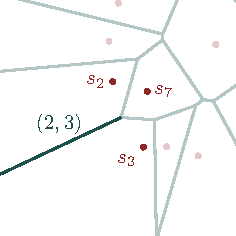
\includegraphics{figures/voronoi/boundary_labels/line/labels.pdf}

}

\subcaption{\label{fig-line-label}}

\end{minipage}%
%
\begin{minipage}{0.33\linewidth}

\centering{

\captionsetup{labelsep=none}
\includegraphics{figures/voronoi/boundary_labels/point/labels.pdf}

}

\subcaption{\label{fig-point-label}}

\end{minipage}%
%
\begin{minipage}{0.01\linewidth}
~\end{minipage}%

\caption{\label{fig-voronoi-labels}(a) Each cell comprising a Voronoi
diagram can be labeled with the unique site that it contains. (b, c)
Similarly the boundaries between neighboring cells can be labeled with
the sites contained by those cells. For the purposes of labeling the the
order of the sites is arbitrary, so \((3, 2)\) is just as good as
\((2, 3)\) while \((2, 7, 3)\), \((3, 7, 2)\), \((3, 2, 7)\),
\((7, 3, 2)\), and \((7, 2, 3)\) are just as good as \((2, 3, 7)\).}

\end{figure}%

\section{The Geometry of Voronoi
Diagrams}\label{the-geometry-of-voronoi-diagrams}

The boundary between the cells of a Voronoi diagram is useful in its own
right. In particular it defines an undirected graph, with linear edges
separating neighboring pairs of cells and punctual vertices separating
neighboring triplets of cells.

Often it is easier in practice to construct this \textbf{Voronoi graph}
and then derive the Voronoi cells from it rather than trying to
construct the Voronoi cells directly. The vertices and edges of the
Voronoi graph exhibit rich geometric structure that provides the
foundation for powerful algorithms.

\subsection{Voronoi Vertices}\label{voronoi-vertices}

The vertices of the Voronoi graph are defined by points that are the
same distance from three neighboring Voronoi cells
(Figure~\ref{fig-vertex}). Consequently we can uniquely label each
vertex with a triplet the sites contained by those cells, \[
(s_{n_{1}}, s_{n_{2}}, w_{n_{3}} ).
\] That said, not every triplet of Voronoi cells are neighbors and not
every triplet of cells defines a valid vertex. Fortunately Euclidean
geometry provides tools for identifying all of the valid vertices.

\begin{figure}

\centering{


\includegraphics[width=0.5\textwidth,height=\textheight]{figures/voronoi/vertex/vertex_distances/vertex.pdf}

}

\caption{\label{fig-vertex}Each vertex in a Voronoi graph is given by a
point on the boundary between three neighboring Voronoi cells. This
point is by definition equally distant to the three sites contained by
those cells.}

\end{figure}%

Each triplet of sites falls onto a unique \textbf{circumcircle} with
center \begin{align*}
x_{c}
&=
\frac{1}{2}
\frac{
  \left( x_{n_{1}}^{2} + y_{n_{1}}^{2} \right) \,
    (y_{n_{2}} - y_{n_{3}})
+ \left( x_{n_{2}}^{2} + y_{n_{2}}^{2} \right) \,
    (y_{n_{3}} - y_{n_{1}})
+ \left( x_{n_{3}}^{2} + y_{n_{3}}^{2} \right) \,
    (y_{n_{1}} - y_{n_{2}})
}{
  x_{n_{1}} \, (y_{n_{2}} - y_{n_{3}} )
+ x_{n_{2}} \, (y_{n_{3}} - y_{n_{1}} )
+ x_{n_{3}} \, (y_{n_{1}} - y_{n_{2}} )
}
\\
y_{c}
&=
\frac{1}{2}
\frac{
  \left( x_{n_{1}}^{2} + y_{n_{1}}^{2} \right) \,
    (x_{n_{3}} - x_{n_{2}})
+ \left( x_{n_{2}}^{2} + y_{n_{2}}^{2} \right) \,
    (x_{n_{1}} - x_{n_{3}})
+ \left( x_{n_{3}}^{2} + y_{n_{3}}^{2} \right) \,
    (x_{n_{2}} - x_{n_{1}})
}{
  x_{n_{1}} \, (y_{n_{2}} - y_{n_{3}} )
+ x_{n_{2}} \, (y_{n_{3}} - y_{n_{1}} )
+ x_{n_{3}} \, (y_{n_{1}} - y_{n_{2}} )
}
\end{align*} and radius \begin{align*}
r
&=
\sqrt{ (x_{c} - x_{n_{1}})^{2} + (y_{c} - y_{n_{1}})^{2} }
\\
&=
\sqrt{ (x_{c} - x_{n_{2}})^{2} + (y_{c} - y_{n_{2}})^{2} }
\\
&=
\sqrt{ (x_{c} - x_{n_{3}})^{2} + (y_{c} - y_{n_{3}})^{2} }.
\end{align*} By construction the center of the circumcircle is
equidistant from all three sites, and hence defines a potential vertex
in the Voronoi graph.

The three sites defining the circumcircle are the three \emph{closest}
sites to this potential vertex if and only if no other sites are inside
of the circumcircle. In other words Voronoi vertices are defined by
\emph{empty} circumcircles.

\begin{figure}

\begin{minipage}{0.17\linewidth}
~\end{minipage}%
%
\begin{minipage}{0.33\linewidth}

\centering{

\captionsetup{labelsep=none}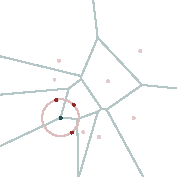
\includegraphics{figures/voronoi/vertex/vertex_good/vertex_good.pdf}

}

\subcaption{\label{fig-vertex-circum-good}}

\end{minipage}%
%
\begin{minipage}{0.33\linewidth}

\centering{

\captionsetup{labelsep=none}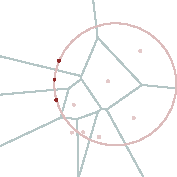
\includegraphics{figures/voronoi/vertex/vertex_bad/vertex_bad.pdf}

}

\subcaption{\label{fig-vertex-circum-bad}}

\end{minipage}%
%
\begin{minipage}{0.17\linewidth}
~\end{minipage}%

\caption{\label{fig-vertex-circum}Not every triplet of sites defines a
vertex in the Voronoi graph. (a) Vertices are defined by triplets of
sites that define empty circumcircless. (b) Triplets of sites whose
circumcircles contain other sites do not define proper vertices.}

\end{figure}%

\subsection{Voronoi Edges}\label{voronoi-edges}

The edges in a Voronoi graph are comprised of points equidistant to two
neighboring cells (Figure~\ref{fig-edge}), allowing us to uniquely label
each Voronoi edge with the pair of sites contained by those cells. Once,
again, however, we have to take care because arbitrary pairs of sites do
not always define valid edges.

\begin{figure}

\centering{


\includegraphics[width=0.5\textwidth,height=\textheight]{figures/voronoi/edge/edge_distances/edge.pdf}

}

\caption{\label{fig-edge}Each edge in a Voronoi graph is defined by
linear boundary between two neighboring Voronoi cells. All of the points
on a Voronoi edge is equally distant to the two sites contained by those
cells.}

\end{figure}%

Before worrying out isolating proper edges let's first work out how to
identify the points that define potential edges. Any pair of sites
defines a line that connects them, and a mid point on that line that is
equally distant to the sites. The \textbf{perpendicular bisector} of two
sites is the line perpendicular to this connecting line that intersects
with the midpoint (Figure~\ref{fig-bisector}). Every point along the
perpendicular bisector between two sites is equally distant from those
two sites and, consequently, could contribute to a Voronoi edge
(Figure~\ref{fig-bisector-edge}).

\begin{figure}

\begin{minipage}{0.17\linewidth}
~\end{minipage}%
%
\begin{minipage}{0.33\linewidth}

\centering{

\captionsetup{labelsep=none}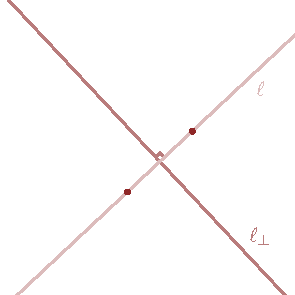
\includegraphics{figures/voronoi/edge/bisector/bisector.pdf}

}

\subcaption{\label{fig-bisector}}

\end{minipage}%
%
\begin{minipage}{0.33\linewidth}

\centering{

\captionsetup{labelsep=none}
\includegraphics{figures/voronoi/edge/bisector_edge/edge.pdf}

}

\subcaption{\label{fig-bisector-edge}}

\end{minipage}%
%
\begin{minipage}{0.17\linewidth}
~\end{minipage}%

\caption{\label{fig-potential-edge}(a) The perpendicular bisector
between two points is the line \(\ell_{\perp}\) that is perpendicular to
line connecting those points \(\ell\) and intersects the midpoint
between them. (b) Every Voronoi edge falls along a perpendicular
bisector between two sites, but not every perpendicular bisector
contains a Voronoi edge and not every point of a perpendicular bisector
that does contain an edge is part of that edge.}

\end{figure}%

In order to determine which segment, if any, of a perpendicular bisector
forms a Voronoi edge we come back to circles. Any point along a
perpendicular bisector is the center of a unique circle that includes
the two defining sites. If no \emph{other} sites are on or inside of
this circle then those two sites are the nearest neighbors to each other
and that point is part of a Voronoi edge.

As we move along the perpendicular bisector these circles will
eventually intersect with another site. When they do the point along the
bisector is equally distant to three sites -- the two initial sites and
this new site -- but the interior of the circle will remain empty. In
other words the Voronoi edge terminates as soon as we hit a Voronoi
vertex.

\begin{figure}

\begin{minipage}{0.01\linewidth}
~\end{minipage}%
%
\begin{minipage}{0.33\linewidth}

\centering{

\captionsetup{labelsep=none}
\includegraphics{figures/voronoi/edge/circle1/edge.pdf}

}

\subcaption{\label{fig-edge-circle1}}

\end{minipage}%
%
\begin{minipage}{0.33\linewidth}

\centering{

\captionsetup{labelsep=none}
\includegraphics{figures/voronoi/edge/circle2/edge.pdf}

}

\subcaption{\label{fig-edge-circle2}}

\end{minipage}%
%
\begin{minipage}{0.33\linewidth}

\centering{

\captionsetup{labelsep=none}
\includegraphics{figures/voronoi/edge/circle3/edge.pdf}

}

\subcaption{\label{fig-edge-circle3}}

\end{minipage}%
%
\begin{minipage}{0.01\linewidth}
~\end{minipage}%

\caption{\label{fig-edge-circles}Circles centered at points along a
perpendicular bisector and intersecting with a pair of sites are useful
for identifying contributions to Voronoi edges. (a) If there are no
other sites on or inside of the circle then the center contributes to a
Voronoi edge. (b) If there is one or more sites inside of the circle
then the center does not contribute to a Voronoi graph at all. (c) If
there is another site on the circle then the center defines a Voronoi
vertex. Each Voronoi edge terminates when these circles first meet a
third site.}

\end{figure}%

\subsection{Voronoi Faces}\label{voronoi-faces}

The edges of a Voronoi graph trace around each site, defining faceted
\textbf{faces} in the graph that correspond to the Voronoi cells
(Figure~\ref{fig-faces}). When working over the entire, unbounded,
Euclidean plane not all of these faces will be closed. While some of the
sites will be entirely fully enclosed by a path of edges, some will be
bounded on only one side by a path of edges. I will refer to these as
closed faces and open faces, respectively.

\begin{figure}

\begin{minipage}{0.17\linewidth}
~\end{minipage}%
%
\begin{minipage}{0.33\linewidth}

\centering{

\captionsetup{labelsep=none}
\includegraphics{figures/voronoi/faces/closed/voronoi.pdf}

}

\subcaption{\label{fig-closed-face}}

\end{minipage}%
%
\begin{minipage}{0.33\linewidth}

\centering{

\captionsetup{labelsep=none}
\includegraphics{figures/voronoi/faces/open/voronoi.pdf}

}

\subcaption{\label{fig-open-face}}

\end{minipage}%
%
\begin{minipage}{0.17\linewidth}
~\end{minipage}%

\caption{\label{fig-faces}The edges of a Voronoi graph trace out faces
which identify the Voronoi cells. (a) I will refer to faces that are
completely enclosed by edges as closed faces and (b) faces that are only
partially enclosed as open faces.}

\end{figure}%

\section{Fortune's Algorithm}\label{fortunes-algorithm}

There are here are multiple ways to construct a Voronoi graph, most of
them suffer from wasteful computation. For large enough numbers of sites
these approaches quickly become too expensive to be practical.
Fortunately there is one elegant approach that, while not at all
initially obvious, is able to construct a Voronoi graph as efficiently
as possible.

\subsection{Inefficient Approaches}\label{inefficient-approaches}

Before diving into efficient solutions let's consider some of the more
straightforward but ultimately inefficient approaches.

One way to identify all of the vertices in a Voronoi graph is to loop
over each triplet of sites and then construct the corresponding
circumcircles. For each of these circumcircles we then loop over the
remaining sites to check for inclusion, with the centers of the empty
circumcircles defining vertices.

We could then construct candidate Voronoi edges by looping over each
pair of sites and scanning across the points between the two Voronoi
vertices associated with those cites. Next we could take any point along
each candidate edge, construct a circle centered on that point and
intersecting with the two associated sites, and check if any other sites
are inside. The candidates with empty circles define Voronoi edges.

Because there are \[
{ N \choose 3 }
=
\frac{ N \, (N - 1) \, (N - 2) }{ 6 }
\] triplets of sites and \[
{ N \choose 2 }
=
\frac{ N \, (N - 1) }{ 2 }
\] pairs of sites to consider, however, the number of operations we need
to implement this brute-force approach scales \emph{cubically} with the
number of sites.

That said, much of this cost is wasted on the repeated querying of each
site; we should be able to construct Voronoi graphs more efficiently if
we can query each site fewer times. One more efficient approach is to
loop over each site, construct the half-planes defined by the
perpendicular bisector between the active site and each other site, and
then construct the corresponding Voronoi face from the intersection of
those half-planes. This cost of this approach requires only quadratic
number of operations.

We can, however, do even better. By systematically scanning across a
plane \textbf{Fortune's algorithm} Berg et al. (2008) is able construct
Voronoi graph with a number of operations proportional to \(N \log N\).
This performance turns out to be theoretically optimal. The main
downside of Fortune's algorithm is that is requires some care to
understand and then implement in a way that achieves that optimal
scaling.

\subsection{The Sweep Line}\label{the-sweep-line}

Fortune's algorithm processes the sites not by working through a list
but rather by systematically scanning across the ambient plane with the
use of a \textbf{sweep line}. Sites on one side of the sweep line are
active and can contribute to the construction of the Voronoi graph while
sites on the other side are inactive and cannot yet contribute. As the
sweep line progresses more sites are processed and more of the Voronoi
graph is built up.

In theory a sweep line can progress in any direction, but most
references consider vertical lines that scan horizontally from left to
right, horizontal lines that scan vertically from top to bottom, or
horizontal lines that scan vertically from bottom to top. These
axis-aligned orientations of the sweep line make geometric calculations
substantially more straightforward.

Here I will consider a vertical sweep line that scans horizontally from
left to right. I will denote the horizontal position of the scan at any
time by \(S\). I will also refer to any site to the left of the sweep
line, \(x_{n} < S\) as active.

\subsection{The Beach Line}\label{the-beach-line}

A sweep line partitions the ambient plane into two pieces, allowing the
construction of the Voronoi graph to focus on just a subset of the
entire plane. That said, not all of the Voronoi graph to the left of the
sweep line is completely determined by the active sites; some features
of the Voronoi diagram can be influenced by sites just beyond the sweep
line.

Consider, for example, a single active site \[
s_{n} = (x_{n}, y_{n})
\] and the sweep line position \[
S > x_{n}.
\] If a point \((x, y)\) on the left of the sweep line is closer to
\(s_{n}\) than the sweep line, \[
(x - x_{n})^{2} - (y - y_{n})^{2} < (S - x)^{2},
\] then we it will be closer to \(s_{n}\) than any other site that might
be hiding beyond the sweep line. On the other any point to the left of
the sweep line that is closer to the sweep line than it is to \(s_{n}\),
\[
(x - x_{n})^{2} - (y - y_{n})^{2} > (S - x)^{2},
\] could be be closer to an inactive site on the other side of the sweep
line.

When determining geometric features such as the nearest sites we cannot
analyze the entire region to the left of the sweep line. Instead we can
analyze only the subset of points that are closer to \(s_{n}\) than they
are to the sweep line. The boundary of this analyzable subset is defined
by the points equidistant to \(s_{n}\) and the sweep line, which traces
out a rotated parabola (Figure~\ref{fig-parabola}) \[
x
=
f(y)
=
\frac{1}{2}
\left( S + x_{n} - \frac{( y - y_{n} )^{2}}{S - x_{n}} \right).
\]

\begin{figure}

\centering{

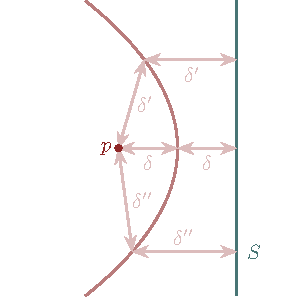
\includegraphics[width=0.5\textwidth,height=\textheight]{figures/fortune/parabola_distances/parabola_distances.pdf}

}

\caption{\label{fig-parabola}The subset of points that are equally
distant from a focus, \(s\), and a vertical line \(S\), form a rotated
parabola. In Fortune's algorithm the points interior to this parabola
are safe to analyze for their contribution to the Voronoi graph.}

\end{figure}%

When there are multiple active sites then the region that we can safely
analyze the points that are closer to \emph{any} of the active sites
than the sweep line. The boundary of this region is defined by the
segmented envelope of the parabolas between each active site and the
sweep line (Figure~\ref{fig-beachline}). Given its resemblance to the
shape made by waves washing up on a beach
(Figure~\ref{fig-actual-beachline}) this boundary is known as the
\textbf{beach line}.

\begin{figure}

\centering{


\includegraphics[width=0.5\textwidth,height=\textheight]{figures/fortune/beachline/beachline.pdf}

}

\caption{\label{fig-beachline}The beach line is the boundary separating
points that are closer to any active site, here \(s_{n_{1}}\),
\(s_{n_{2}}\), and \(s_{n_{3}}\), and points that are closer to the the
sweep line, \(S\), is comprised of multiple parabolic arcs. Note that
the parabola between \(s_{n_{1}}\) and \(S\) contributes multiple arcs
to the beach line here.}

\end{figure}%

\begin{figure}

\centering{

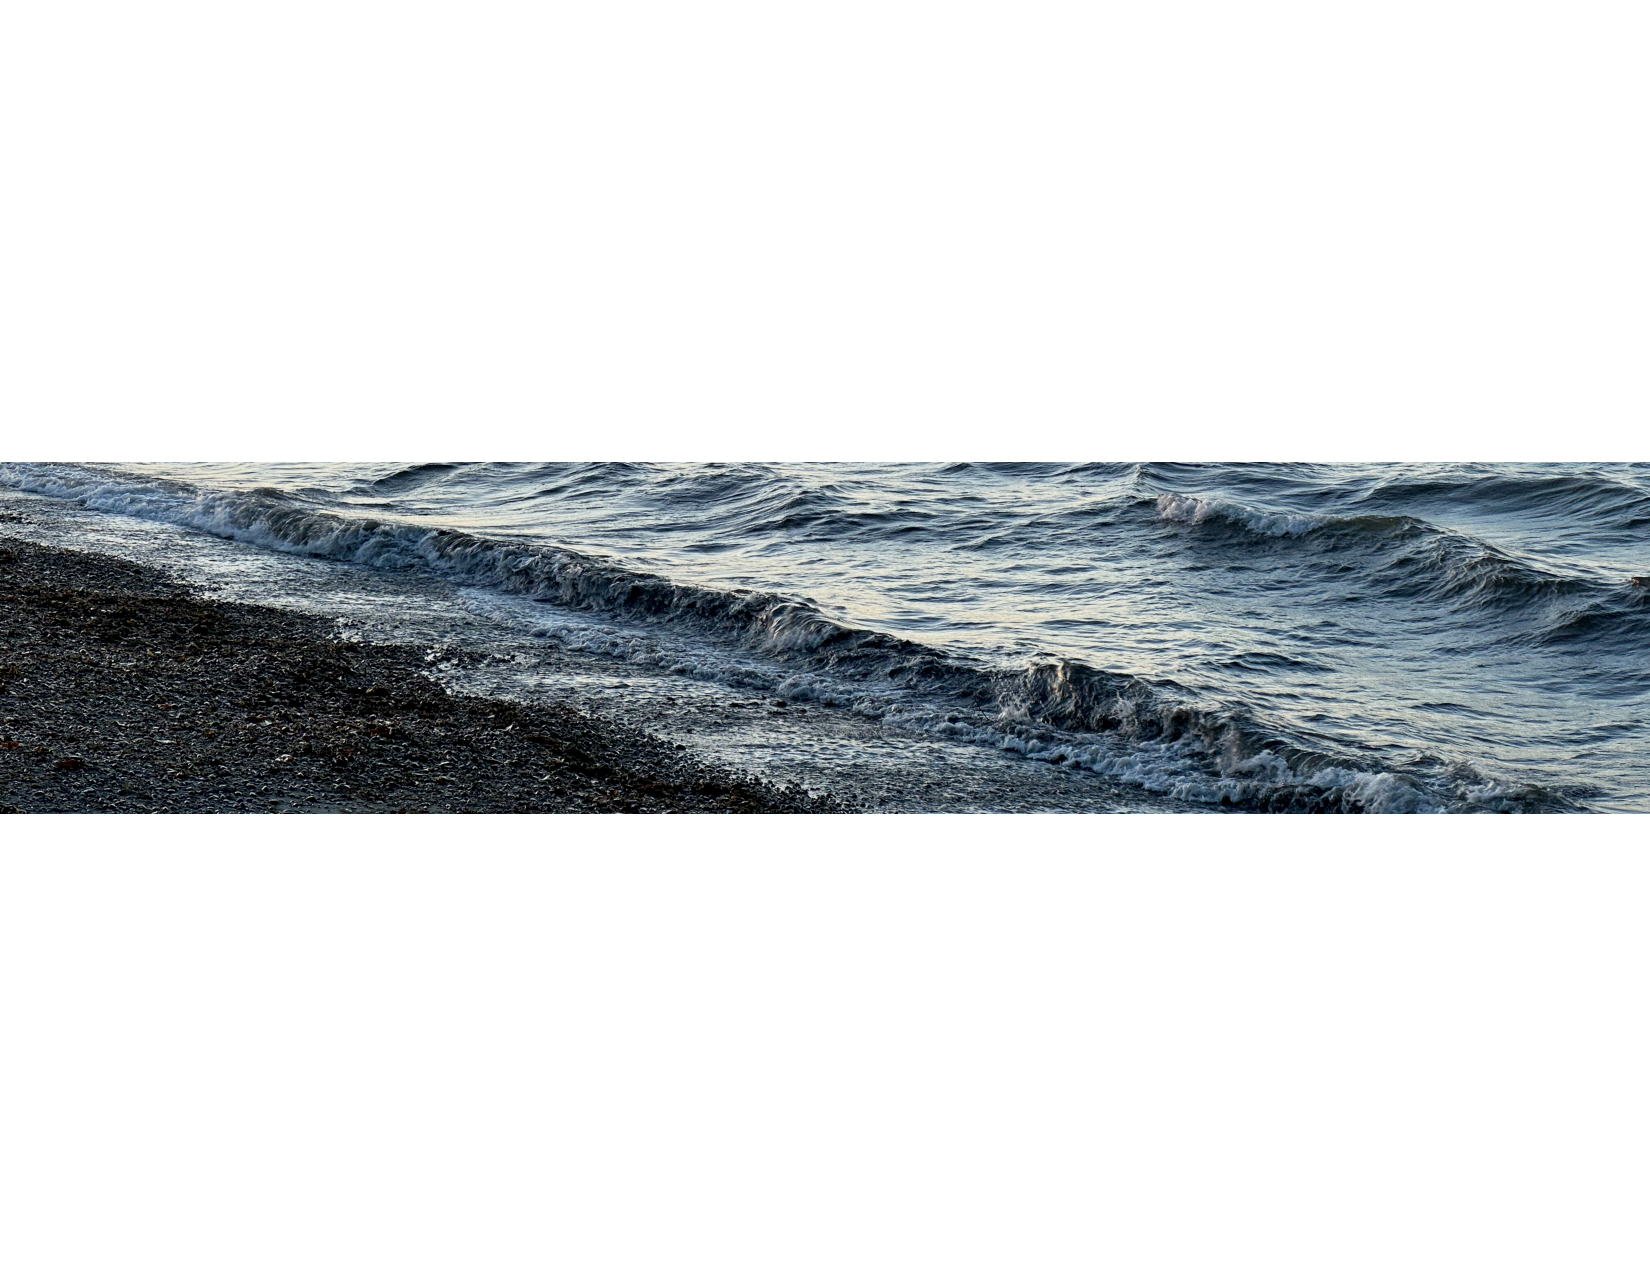
\includegraphics[width=1\textwidth,height=\textheight]{figures/fortune/actual_beachline/actual_beachline.pdf}

}

\caption{\label{fig-actual-beachline}The parabolic arcs that make up a
beach line are similar to the shape made by waves washing up onto a
beach, hence the name.}

\end{figure}%

Each parabolic segment, or \textbf{arc}, in a beach line is associated
with a single site. The parabola between each site and the sweep line,
however, can contribute to the beach line multiple times. Consequently
we cannot use the originating sites to \emph{uniquely} label the arcs.

By construction neighboring arcs on the beach line are derived from
neighboring sites. The discontinuities along the beach line that
separate each pair of neighboring arcs are known as \textbf{breakpoints}
(Figure~\ref{fig-breakpoints}). Each breakpoint is uniquely labeled by
an ordered pair of the sites associated with those arcs. Ordering is
important here: \((s_{n_{1}}, s_{n_{2}})\) and
\((s_{n_{2}}, s_{n_{1}})\) correspond to two \emph{different}
breakpoints.

\begin{figure}

\centering{

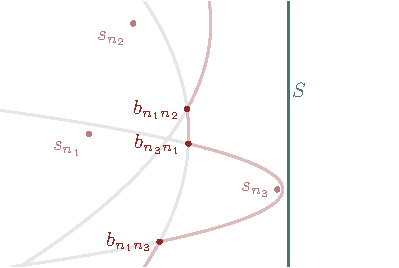
\includegraphics[width=0.5\textwidth,height=\textheight]{figures/fortune/breakpoints/breakpoints.pdf}

}

\caption{\label{fig-breakpoints}The breakpoints in a beach line separate
the component arcs. Each breakpoint is located at the intersection
between the parabolas defined by two neighboring sites, equally distant
from those two sites and further from any other sites. We can use an
ordered pair of these sites to uniquely label each breakpoint.}

\end{figure}%

Given a sweep line configuration we can readily calculate the
intersection of each pair of neighboring parabolas and hence the
position of any given breakpoint. Formally if the lower arc is a segment
of the parabola generated by \(s_{n_{1}}\) and the higher arc is a
segment of the parabola generated by \(s_{n_{2}}\) then the vertical
position of the breakpoint between those arcs is given by one of the two
solutions to the quadratic equation \begin{align*}
0
&=\quad
\Bigg( x_{n_{2}} - x_{n_{1}} \Bigg) \, y_{n_{1}n_{2}}^{2}
\\
&\quad
+
\Bigg(  y_{n_{2}} \, (S - x_{n_{1}})
      - y_{n_{1}} \, (S - x_{n_{2}}) \Bigg) \, y_{n_{1}n_{2}}
\\
&\quad
+
\Bigg(  y_{n_{2}}^{2} \, (S - x_{n_{1}})
      - y_{n_{1}}^{2} \, (S - x_{n_{2}})
      - (S - x_{n_{1}}) \,
        (S - x_{n_{2}}) \,
        (x_{n_{2}} - x_{n_{1}} ).
\Bigg)
\end{align*} The correct solution is the one that falls in between the
height of the two neighboring sites, \[
y_{n_{1}} < y_{n_{1}n_{2}} < y_{n_{2}}.
\]

When it comes to constructing Voronoi graphs the breakpoints are the
most important part of the beach line. Because each breakpoint falls
onto the parabolas of two neighboring sites, it is equally distant from
those two sites and the sweep line. At the same time no other active
site is closer than those two sites, otherwise the parabolas generated
by them would not define neighboring arcs on the beach line. In addition
every inactive site is also further because they're all beyond the sweep
line.

All of this is to say that, by construction, each breakpoint is the
center of a circle that intersects with the two associated sites but
includes no other sites. Consequently each breakpoint \emph{is always a
part of a Voronoi edge}.

\subsection{Evolving The Beach Line}\label{evolving-the-beach-line}

As we scan the sweep line across a Euclidean plane the distances between
the active sites and the sweep line change. This in turn changes the
shape of the corresponding parabolas, and hence the shape of the beach
line. As the beach line evolves in this way the breakpoints trace out
the edges of the Voronoi diagram.

Every now and then the number of arcs comprising the beach line,
referred to as the \textbf{topology} of the beach line, also changes.
When the sweep line passes over a new site, for example, a new arc is
added to the beach line. Similarly arcs can be removed from the beach
line when they are squeezed to a point by their neighboring arcs.

Conveniently we don't need to continuously scan the sweep line in order
to construct a Voronoi diagram. All of the information we need is
completely determined by the behavior of the beach line at the finite
number of sweep line positions where the topology changes. If we can
efficiently determine these topology-changing \textbf{events} then we
can efficiently build up a Voronoi diagram in a finite number of
operations.

\subsubsection{Events Where The Beach Line
Expands}\label{events-where-the-beach-line-expands}

Whenever the sweep line crosses a new site that site becomes active and
contributes a new parabolic arc to the beach line. Because we know the
position of all of the sites in advance we at exactly which positions
these \textbf{site events} will occur.

If the sweep line falls exactly on a new site then the parabola of
points equidistant from the site and the sweep line is singular,
consisting of just the new site itself. This forms a point discontinuity
with the rest of the beach line (Figure~\ref{fig-site-event1a}).
Although not \emph{technically} correct, these singular arcs are often
visualized with a horizontal line extending from the new site to the
beach line (Figure~\ref{fig-site-event1b}).

\begin{figure}

\begin{minipage}{0.01\linewidth}
~\end{minipage}%
%
\begin{minipage}{0.33\linewidth}

\centering{

\captionsetup{labelsep=none}
\includegraphics{figures/fortune/site_event/1a/site_event.pdf}

}

\subcaption{\label{fig-site-event1a}}

\end{minipage}%
%
\begin{minipage}{0.33\linewidth}

\centering{

\captionsetup{labelsep=none}
\includegraphics{figures/fortune/site_event/1b/site_event.pdf}

}

\subcaption{\label{fig-site-event1b}}

\end{minipage}%
%
\begin{minipage}{0.33\linewidth}

\centering{

\captionsetup{labelsep=none}
\includegraphics{figures/fortune/site_event/2/site_event.pdf}

}

\subcaption{\label{fig-site-event2}}

\end{minipage}%
%
\begin{minipage}{0.01\linewidth}
~\end{minipage}%

\caption{\label{fig-site-event}At a site event the sweep line passes an
inactive site which then becomes active. (a) Initially the new active
site introduces a new singular arc which forces a discontinuity in the
beach line. (b) This singular arc is often visualized with a straight
line. (c) As the sweep line proceeds past the site event the singular
arc widens into a well-behaved parabola, splitting one of the initial
beach line arcs into a triplet of arcs.}

\end{figure}%

As the sweep line progresses past the new active site the singular
parabola widens into a more well-behaved parabola
(Figure~\ref{fig-site-event2}). This not only restores the continuity of
the beach line but also splits an existing parabolic arc into two new
arcs. The introduction of a new active site always splits an existing
arc into a triplet of arcs.

For example let's say that the sweep line passes the new site
\(s_{n_{2}}\). If the height of this site \(y_{n_{2}}\) intersects with
an arc generated by the site \(s_{n_{1}}\) then the site event will
split that arc into a triplet of arcs, the outer two of which are
generated by \(s_{n_{1}}\) and the center of which is generated by
\(s_{n_{2}}\). These three arcs are separated by two new breakpoints
\(b_{ n_{1} n_{2} }\) and \(b_{ n_{2} n_{1} }\).

Both of the breakpoints fall onto a Voronoi edge in between the sites
\(s_{n_{1}}\) and \(s_{n_{2}}\). As the sweep line progresses the middle
arc widens and the breakpoints \(b_{ n_{1} n_{2} }\) and
\(b_{ n_{2} n_{1} }\) separate, tracing out more and more of the edge
(Figure~\ref{fig-site-event-breakpoints})

\begin{figure}

\centering{


\includegraphics[width=0.5\textwidth,height=\textheight]{figures/fortune/site_event/breakpoints/breakpoints.pdf}

}

\caption{\label{fig-site-event-breakpoints}As the sweep line moves past
a site event the two new breakpoints separate and scan across the
Voronoi edge between the two neighboring sites.}

\end{figure}%

\subsubsection{Events Where The Beach Line
Contracts}\label{events-where-the-beach-line-contracts}

The topology of the beach line can also change when one of the parabolic
arcs collapses in between its two neighboring arcs
(Figure~\ref{fig-vertex-event-collapse}). In this case the collapsed arc
is removed from the beach line and its two neighbors become neighbors
themselves.

\begin{figure}

\centering{


\includegraphics[width=0.5\textwidth,height=\textheight]{figures/fortune/vertex_event/collapse/vertex_event.pdf}

}

\caption{\label{fig-vertex-event-collapse}As the sweep line progresses
arcs on the beach line can collapse in between their two neighboring
arcs, with the neighboring breakpoints converging to a point. This point
is equally distant from the three active sites and further from all
other sites, defining a vertex in the Voronoi graph.}

\end{figure}%

Now an arc in between two arcs that are generated from the same active
site, such as the central arc introduced when the sweep line crosses a
site event, always widens faster than its neighboring arcs as the sweep
line progresses. Consequently a triplet of arcs generated by only two
sites, \((s_{n_{1}}, s_{n_{2}}, s_{n_{1}})\), will never collapse.
Rather collapsing arcs are \emph{always} defined by triplets of arcs
generated by three distinct sites,
\((s_{n_{1}}, s_{n_{2}}, s_{n_{3}})\).

When the central arc collapses its two neighboring breakpoints
\(b_{ n_{1} n_{2} }\) and \(b_{ n_{2} n_{3} }\) will intersect. At that
moment the breakpoints are equally distant from the sweep line and all
tree of the associated sites, \(s_{n_{1}}\), \(s_{n_{2}}\), and
\(s_{n_{3}}\) . Moreover, because this intersection is on the beach line
it cannot be closer to any in active sites hiding beyond the sweep line.
In other words a collapsing arc on the beach line always defines a
Voronoi vertex.

This duality between arc collapses and Voronoi vertices is useful not
only for building up the Voronoi graph but also for predicting when arcs
will collapse. At this point it should not be a surprise that this
prediction will involve circles.

For any triplet of neighboring arcs on a beach line that correspond to
the \emph{distinct} sites \((s_{n_{1}}, s_{n_{2}}, s_{n_{3}})\) we can
always construct a unique circumcircle with center \((x_{c}, y_{c})\)
and radius \(r\). By construction the center \((x_{c}, y_{c})\) is
equally distant to all three sites. The center is also equally distant
to vertical lines at \(x = x_{c} - r\) and \(x = x_{c} + r\).
Consequently if the central arc collapses then it will do so when the
sweep line is at either \(S = x_{c} - r\) or \(S = x_{c} + r\)
(Figure~\ref{fig-vertex-event-circumcircle}).

\begin{figure}

\centering{


\includegraphics[width=0.5\textwidth,height=\textheight]{figures/fortune/vertex_event/circumcircle/vertex_event.pdf}

}

\caption{\label{fig-vertex-event-circumcircle}If the central arc in a
triplet of neighboring arcs generated by distinct sites will collapse
then it will do so when the sweep line is at the far edge of the
circumcircle spanned by those tree sites. This geometric extrapolation
allows us to schedule future vertex events.}

\end{figure}%

A collapse at \(S = x_{c} - r\) can't contribute information about the
Voronoi graph because it is ahead of the current beach line where the
structure of the Voronoi graph has already been established. If the
central arc collapses at this point then it will \emph{expand} as the
sweep line progresses further.

Instead we can focus on a new \textbf{vertex event}, also known as a
\textbf{circle event}, at \(S = x_{c} + r\). If the the central arc
generated by \(s_{n_{2}}\) collapses when the sweep line reaches this
position then \(b_{ n_{1} n_{2} }\) and \(b_{ n_{2} n_{3} }\) will
intersect at \((x_{c}, y_{c})\). In turn this intersection defines a new
vertex that we can add to the Voronoi graph
(Figure~\ref{fig-vertex-event-voronoi}).

\begin{figure}

\centering{


\includegraphics[width=0.5\textwidth,height=\textheight]{figures/fortune/vertex_event/voronoi/voronoi.pdf}

}

\caption{\label{fig-vertex-event-voronoi}When a central arc collapses
two Voronoi edges terminate at a Voronoi edge and a new Voronoi edge
between the sites that generate the remaining arcs is created.}

\end{figure}%

\subsection{The Algorithm}\label{the-algorithm}

Now that we know how and when the topology of a beach line can change we
can organize those changes into a dynamic algorithm that builds up a
Voronoi graph dynamically.

Fortune's algorithm starts with an \textbf{event queue} consisting of
events defined by sweep line positions where an arc is added to or
removed from the beach line. The algorithm then proceeds iteratively,
processing the next event in the queue to expand the structure of the
Voronoi graph and add new events as necessary. Initially the event queue
is filled with only site events, one for each site, and vertex events
are added as the site events are processed.

In this section we'll review the basic steps required to process both
site and vertex events, as well as clean up after the event queue has
been fully processed. The details depend on how we implement Fortune's
algorithm, which will be the focus of the next section.

\subsubsection{Site Events}\label{site-events}

Processing a site event requires adding a new arc to the beach line. To
do this we have to scan across the current beach line to find the
existing arc at the same height as the new event. We then split that arc
in two, inserting a new arc generated by the new site into the beach
line along with two new breakpoints.

Inserting a new arc into the beach line can also modify the remaining
event queue. For example inserting a new arc will disrupt some of the
triplets of neighboring arcs generated by distinct sites in the previous
beach line. If any of those arc triplets correspond to a future vertex
events in the event queue then they have have to be removed.

At the same time inserting a new arc also creates new triplets of
neighboring arcs, each of which could potentially spawn a vertex event.
After checking that the individual arcs are generated by distinct sites
we have to check whether or not the central arc actually collapses
beyond the current sweep line. If all of these conditions are met then
we add a new vertex event to the event queue where the central arc will
be removed.

\subsubsection{Vertex Events}\label{vertex-events}

When we encounter a vertex event we first have to remove the central arc
from the beach line, along with one of its neighboring breakpoints.

At this point we expand the current Voronoi graph. This starts by adding
a new Voronoi vertex, connecting it to two of the previously dandling
Voronoi edges, and then creating a new Voronoi edge. Exactly how we
accomplish this depends on how the graph is implemented.

Lastly we have to clean up the event queue. The removal of the central
arc, for example, will invalidate any vertex event in the remaining
event queue where the central arc was previously neighbors with the
removed arc. On the other hand the removal also creates two new triplets
of neighboring arcs along the beach line, each of which could spawn a
new vertex event. If any of these triplets consist of arcs generated by
distinct sites with the central arc collapses beyond the current sweep
line then we add a corresponding vertex event to the event queue.

\subsubsection{Clean Up}\label{clean-up}

As we process the events the event queue will eventually empty. When
there are no more events to process the algorithm will have found all of
the Voronoi vertices and all of the Voronoi edges. That said some of
those edges will be dangling, anchored to a vertex on only one side
because they stretch out to infinity (Figure~\ref{fig-clean-up1}).

\begin{figure}

\begin{minipage}{0.01\linewidth}
~\end{minipage}%
%
\begin{minipage}{0.33\linewidth}

\centering{

\captionsetup{labelsep=none}
\includegraphics{figures/fortune/cleanup/dangling/voronoi.pdf}

}

\subcaption{\label{fig-clean-up1}}

\end{minipage}%
%
\begin{minipage}{0.33\linewidth}

\centering{

\captionsetup{labelsep=none}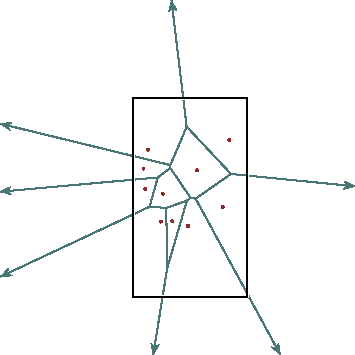
\includegraphics{figures/fortune/cleanup/bounding_box/voronoi.pdf}

}

\subcaption{\label{fig-clean-up2}}

\end{minipage}%
%
\begin{minipage}{0.33\linewidth}

\centering{

\captionsetup{labelsep=none}
\includegraphics{figures/fortune/cleanup/pseudo_vertices/voronoi.pdf}

}

\subcaption{\label{fig-clean-up3}}

\end{minipage}%
%
\begin{minipage}{0.01\linewidth}
~\end{minipage}%

\caption{\label{fig-clean-up}(a) After running Fortune's algorithm some
of the edges in the Voronoi graph will be connected to vertices on only
one side. The other side dangles out towards infinity. (b) When
visualizing a Voronoi graph we can consider only a finite range of
values. This requires limiting the visualization to a bounding box that
contains all of the Voronoi vertices. (c) For visualization purposes we
can anchor the dangling edges to points where they meet the bounding
box.}

\end{figure}%

We can handle these dangling edges in a few different ways. For example
from a graph theory perspective we can anchor any dangling edges to a
single ``vertex at infinity'' that quantifies the common unboundedness
of those edges. This approach, however, does not yield particularly
compelling visualizations.

For visualization purposes it is more useful to create a
\textbf{bounding box} that contains all of the Voronoi vertices, and
ideally all of the sites, (Figure~\ref{fig-clean-up2}) and then anchor
the dandling edges to points along this rectangle
(Figure~\ref{fig-clean-up3}). Specifically the anchor for a dangling
edge will be at the point where the perpendicular bisector between the
two sites associated with the edge intersect with the bounding box.

\section{Implementing Fortune's
Algorithm}\label{implementing-fortunes-algorithm}

Once we've built up enough familiarity with planar geometry, the
motivation for Fortune's algorithm, particularly the utility of a beach
line and its evolution, becomes less obscure. That said, there is still
work to do to ensure that we can implement the algorithm in a way that
achieves the maximum possible performance.

For example when processing a site event we need to be able to
efficiently search through the arcs on the current beach line. If we
naively scan through the \emph{entire} beach line every time we process
a new site event then the the number of operations needed to implement
Fortune's algorithm with scale with not \(N \log N\) but rather
\(N^{2}\). To achieve that \(N \log N\) scaling we need to implement the
beach line in a way that allows for efficient searching.

Similarly we need to keep track of the next event while we add and
delete events from the event queue. We could accomplish this by sorting
the entire event queue after every update, but this is wasteful and
spoils the optimal \(N \log N\) scaling.

Fortunately (pun very much intended) if we leverage some standard data
structures from computer science then we can avoid these potential
slowdowns and implement Fortune's algorithm as efficiently as possible.

\subsection{Implementing Voronoi
Graphs}\label{implementing-voronoi-graphs}

In theory graphs are straightforward to specify with a just list of
points for each vertex and list of pairs of points for each edge. While
these lists allow us to draw a graph easily enough, they don't provide
enough information to perform basic graph operations, such as tracing
along paths of edges to derive faces.

The \textbf{doubly-connected edge list} (Berg et al. 2008) is a data
structure that efficiently captures not only the components of a graph
but also the relationships between those components. These relationships
in turn make it straightforward to efficiently implement basic graph
algorithms.

A doubly-connected edge list is itself built up from lists of three
primitive data structures: half-edges, vertices, and faces.

\subsubsection{Half-Edges}\label{half-edges}

Doubly-connected edge lists don't represent undirected edges directly.
Instead the data structure splits undirected edges into two directed
edges known as \textbf{half-edges} (Figure~\ref{fig-dcel-half-edge}).

\begin{figure}

\centering{

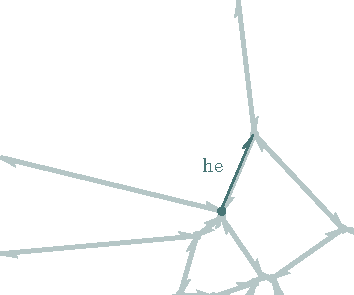
\includegraphics[width=0.5\textwidth,height=\textheight]{figures/dcel/half_edge/1/edge.pdf}

}

\caption{\label{fig-dcel-half-edge}Doubly-connected edge lists represent
undirected edges with a pair of directed half-edges. Each half-edge
includes references to other structures in the doubly-connected edge
lists, including the vertex from which the half-edge originates and
neighboring half-edges.}

\end{figure}%

To situate them within the full graph, each half-edge is endowed with a
collection of references to other objects in the doubly-connected edge
list. For example each half-edge includes a reference to the vertex from
which the half-edge originates. Similarly each half-edge includes
references to three other half-edges -- the \emph{previous} half-edge
that points into it, the \emph{next} half-edge that it points into, and
the \emph{twin} half-edge that completes it to form a full undirected
edge (Figure~\ref{fig-dcel-half-edge-refs}). Finally each half-edge
includes a reference to the face located to the left of the half-edge.

\begin{figure}

\centering{


\includegraphics[width=0.5\textwidth,height=\textheight]{figures/dcel/half_edge/2/edge.pdf}

}

\caption{\label{fig-dcel-half-edge-refs}Each half-edge in a
doubly-connected edge lists includes reference three other half-edges.
The previous half-edge, here labeled ``he.prv'', identifies the
half-edge that points into it while the next half-edge, here labeled
``he.nxt'', identifies the half-edge that it points into. Finally the
twin half-edge, here labeled ``he.twin'', identifies the half-edge that
completes it to form a full undirected edge.}

\end{figure}%

These references make a variety of graph operations straightforward to
implement. For instance the originating vertex and twin half-edge
references provide enough information to draw a half-edge as a directed
line segment, starting at the position of the originating vertex and
then ending at the position of the twin's originating vertex.

Similarly we can use the previous and next references to trace through
paths in the graph. These paths can then be used to quantify topological
information about the graph, such as the configuration of the faces.

Voronoi graphs generally feature unbounded edges, with only one side
terminating at a vertex and the other shooting off towards infinity. In
this case some of the half-edges will feature empty next half-edge
references and their twins will features empty originating vertices and
previous half-edge references.

\subsubsection{Vertices}\label{vertices}

Each vertex in a doubly-connected edge list is specified with its
spatial position and a reference to any one half-edge that originates
from it (Figure~\ref{fig-dcel-vertex}). The relationship of a vertex to
the rest of graph can be completely reconstructed from this information
alone.

\begin{figure}

\centering{

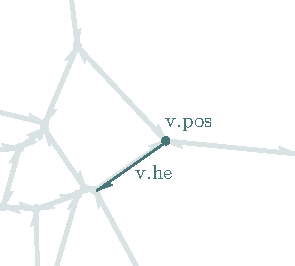
\includegraphics[width=0.5\textwidth,height=\textheight]{figures/dcel/vertex1/vertex.pdf}

}

\caption{\label{fig-dcel-vertex}Each vertx in a doubly-connected edge
list includes its spatial position, here denoted ``v.pos'' and a
reference to any one half-edge that originates from it, here denoted
``v.he''.}

\end{figure}%

For example all of the half-edges that originate at a given vertex can
always be accessed by repeatedly following the twin and next references
from the included half-edge (Figure~\ref{fig-dcel-vertex-algo}).
Equivalently we can iteratively follow the previous and then twin
references. In the same way we can access the half-edges that
\emph{terminate} at a given vertex.

\begin{figure}

\begin{minipage}{0.50\linewidth}

\centering{

\captionsetup{labelsep=none}
\includegraphics{figures/dcel/vertex2/1/vertex.pdf}

}

\subcaption{\label{fig-dcel-vertex-algo1}}

\end{minipage}%
%
\begin{minipage}{0.50\linewidth}

\centering{

\captionsetup{labelsep=none}
\includegraphics{figures/dcel/vertex2/2/vertex.pdf}

}

\subcaption{\label{fig-dcel-vertex-algo2}}

\end{minipage}%
\newline
\begin{minipage}{0.50\linewidth}

\centering{

\captionsetup{labelsep=none}
\includegraphics{figures/dcel/vertex2/3/vertex.pdf}

}

\subcaption{\label{fig-dcel-vertex-algo3}}

\end{minipage}%
%
\begin{minipage}{0.50\linewidth}

\centering{

\captionsetup{labelsep=none}
\includegraphics{figures/dcel/vertex2/4/vertex.pdf}

}

\subcaption{\label{fig-dcel-vertex-algo4}}

\end{minipage}%

\caption{\label{fig-dcel-vertex-algo}(a) The one half-edge referenced in
a vertex object is enough to reconstruct the entire structure of the
graph around that vertex. For example if we follow the reference to (b)
the previous half-edge, ``v.he.p'', (c) and then its twin, ``v.he.p.t'',
we recover another half-edge that originates from that vertex. (d)
Repeating this operation recovers all of the half-edges that originate
from that vertex.}

\end{figure}%

Once we can access all of the neighboring half-edges we can then access
additional information about the local structure of the graph.
Neighboring vertices, for instance, are immediately given by the
originating vertex references of the twin of any half-edge that
originates at a given vertex.

\subsubsection{Faces}\label{faces}

Finally each face in the graph is specified by any one half-edge along
its boundary (Figure~\ref{fig-dcel-face1}). The provides enough
information to trace out the entire boundary by following the next or
previous references from that one included half-edge
(Figure~\ref{fig-dcel-face2}, Figure~\ref{fig-dcel-face3}).

\begin{figure}

\begin{minipage}{0.01\linewidth}
~\end{minipage}%
%
\begin{minipage}{0.33\linewidth}

\centering{

\captionsetup{labelsep=none}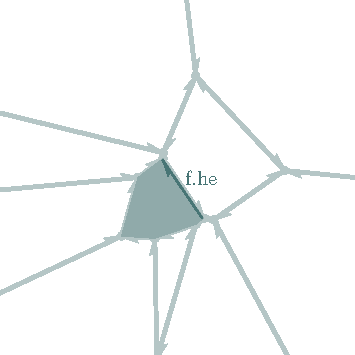
\includegraphics{figures/dcel/face1/face.pdf}

}

\subcaption{\label{fig-dcel-face1}}

\end{minipage}%
%
\begin{minipage}{0.33\linewidth}

\centering{

\captionsetup{labelsep=none}
\includegraphics{figures/dcel/face2/face.pdf}

}

\subcaption{\label{fig-dcel-face2}}

\end{minipage}%
%
\begin{minipage}{0.33\linewidth}

\centering{

\captionsetup{labelsep=none}
\includegraphics{figures/dcel/face3/face.pdf}

}

\subcaption{\label{fig-dcel-face3}}

\end{minipage}%
%
\begin{minipage}{0.01\linewidth}
~\end{minipage}%

\caption{\label{fig-dcel-face}(a) Each face in a doubly-connected edge
list includes a references to any one half-edge along its boundary. By
following the next and previous references from that one half-edge we
can always trace out the entire boundary of the face, regardless of
whether the face is (b) closed or (c) open.}

\end{figure}%

When working with graphs that contain disconnected faces or faces that
are completely surrounded by other faces, also known as holes, we would
need to include additional half-edge references, such as one along
exterior boundary and one along each internal boundary. Because Voronoi
graphs do not exhibit these topological features, however, we don't need
to worry about this additional information.

\subsubsection{Satellite Data}\label{satellite-data}

Depending upon the application the half-edge, vertex, and face data
structures can also include additional information in the form of
\textbf{satellite data}. For example when using a doubly-connected edge
list to represent a Voronoi graph it will be helpful to include
information about the associated sites, three for each vertex objects
and one for each face object. We don't need to store the two sites
associated with an edge, as these can be recovered from the sites of the
left faces of the corresponding half-edges.

\subsubsection{Bounding Box and
Pseudo-Vertices}\label{bounding-box-and-pseudo-vertices}

The visualization of Voronoi graphs is easier if we add a few more
objects to the doubly-connected edge list data structure. In particular
we will add the configuration of a bounding box as well as
\textbf{pseudo-vertices} along that bounding box that can be used to
terminate any dangling half-edges. This ensures that every half-edge
includes a non-empty originated vertex references which in turns makes
visualization functions more uniform.

\subsection{Implementing Beach Lines}\label{implementing-beach-lines}

A beach line consists of parabolic arcs and separated breakpoints, all
of which \emph{ordered}. As we work through Fortune's algorithm we'll
need to be able to not only add and remove arcs and breakpoints but also
efficiently search through these ordered objects. All of these
operations can be implemented with a slightly modified \textbf{binary
search tree} (Cormen et al. 2022) where each node represents either an
arc or a breakpoint (Figure~\ref{fig-bst}).

\begin{figure}

\begin{minipage}{0.25\linewidth}
~\end{minipage}%
%
\begin{minipage}{0.50\linewidth}

\centering{

\captionsetup{labelsep=none}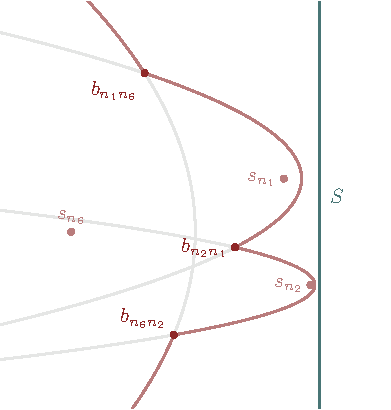
\includegraphics{figures/bst/beachline/beachline.pdf}

}

\subcaption{\label{fig-bst-beachline}}

\end{minipage}%
%
\begin{minipage}{0.25\linewidth}
~\end{minipage}%
\newline
\begin{minipage}{\linewidth}

\centering{

\captionsetup{labelsep=none}
\includegraphics{figures/bst/bst/bst.pdf}

}

\subcaption{\label{fig-bst-bst}}

\end{minipage}%

\caption{\label{fig-bst}Every (a) beach line can be implemented with a
(b) slightly modified binary search tree where internal nodes represent
the breakpoints in the beach line and leaf nodes represent the arcs.
Critically the ordering of nodes in the binary tree preserves the
spatial relationships of the objects in the beach line. This main
difference between this binary search tree and a standard binary search
is a lack of static keys within each node.}

\end{figure}%

\subsubsection{Arc Nodes}\label{arc-nodes}

When using a binary search tree to represent a beach line each arc is
represented by a non-empty leaf node. I will refer to these as
\textbf{arc nodes}.

\begin{figure}

\begin{minipage}{0.25\linewidth}
~\end{minipage}%
%
\begin{minipage}{0.50\linewidth}

\centering{

\captionsetup{labelsep=none}
\includegraphics{figures/bst/beachline_arcs/beachline.pdf}

}

\subcaption{\label{fig-bst-beachline-arc}}

\end{minipage}%
%
\begin{minipage}{0.25\linewidth}
~\end{minipage}%
\newline
\begin{minipage}{\linewidth}

\centering{

\captionsetup{labelsep=none}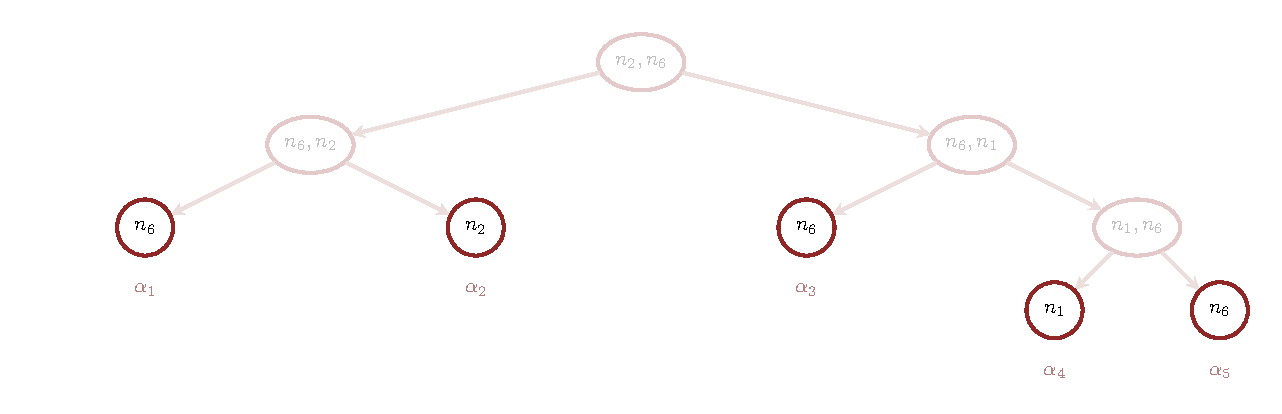
\includegraphics{figures/bst/arc_nodes/arc_nodes.pdf}

}

\subcaption{\label{fig-bst-bst-arc}}

\end{minipage}%

\caption{\label{fig-bst-arc}(b) Each leaf node in the binary search tree
corresponds to (a) a parabolic arc in the beach line. Because of the
shape of these arcs changes with the position of the sweep line these
arc nodes do not include any geometric information. Instead they include
a reference to the site that generates the arc which then allows us to
calculate the current arc shape whenever necessary.}

\end{figure}%

Beyond a reference to their parent nodes, each of these arc nodes also
contain a reference to the site that generates the arc. This allows us
to, for example, dynamically compute the shape of the arc for any
position of the sweep line. Because the parabola generated by a single
site can contribute to the beach line multiple times, multiple arc nodes
can share the same site reference.

To avoid having to search through the event queue we also include in
each arc node a reference to any vertex events that centered on that
arc. This allows us to, for example, quickly find events that need to be
removed from the event queue.

\subsubsection{Breakpoint Nodes}\label{breakpoint-nodes}

The internal nodes of a binary search tree represent the breakpoints
between the arcs in a beach line. I will unsurprisingly refer to these
as \textbf{breakpoint nodes}.

\begin{figure}

\begin{minipage}{0.25\linewidth}
~\end{minipage}%
%
\begin{minipage}{0.50\linewidth}

\centering{

\captionsetup{labelsep=none}
\includegraphics{figures/bst/beachline_bps/beachline.pdf}

}

\subcaption{\label{fig-bst-beachline-bp}}

\end{minipage}%
%
\begin{minipage}{0.25\linewidth}
~\end{minipage}%
\newline
\begin{minipage}{\linewidth}

\centering{

\captionsetup{labelsep=none}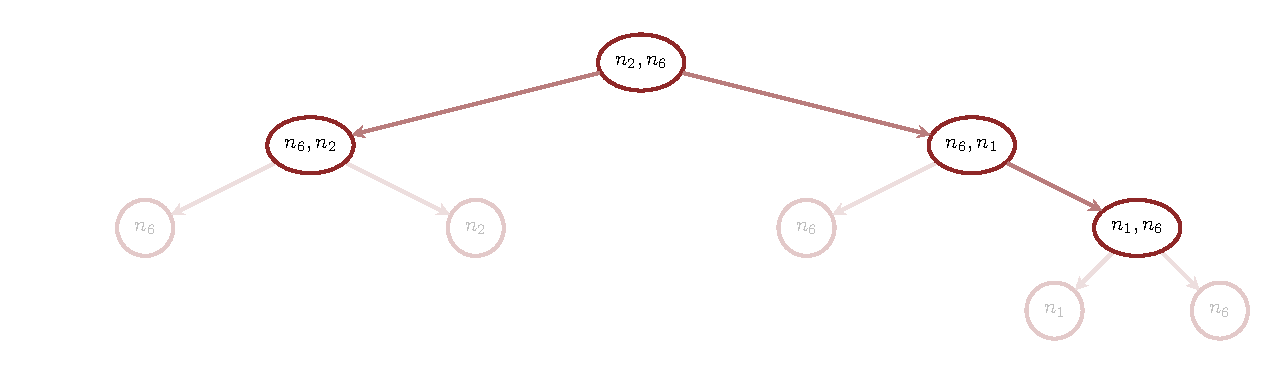
\includegraphics{figures/bst/bp_nodes/bp_nodes.pdf}

}

\subcaption{\label{fig-bst-bst-bp}}

\end{minipage}%

\caption{\label{fig-bst-bp}(b) Each internal node in the binary search
tree corresponds to (a) a breakpoint on the beach line. These nodes are
equipped with references to the two neighboring sites as well as a
reference to one Voronoi half-edge.}

\end{figure}%

As with any binary search tree, each internal node contains references
to theirs parents and children in the tree. When implementing Fortune's
algorithm we will also need to augment the internal nodes with
additional satellite data.

Firstly we'll need to include a reference to the two sites that generate
the neighboring arcs on each side of the breakpoint. This information
allows us to dynamically calculate the position of each breakpoint for
any position of the sweep line. Unlike the site references in the arc
nodes, these ordered pairs of sites uniquely label each breakpoint node.

We will also use the breakpoint nodes to store incomplete Voronoi edges.
Because there are always two breakpoints that fall on the same Voronoi
edge, however, we can't store a unique edge in each breakpoint node.
What we can do is split each edge into half-edges and then store a
unique half-edge in each breakpoint node. This makes the implementation
of Fortune's algorithm more symmetric.

As the sweep line progresses these incomplete half-edges will not yet
have an originating vertex. For visualization purposes we can always
display these half-edges as if they originated from the current position
of the corresponding breakpoint (Figure~\ref{fig-bst-edges}).

\begin{figure}

\centering{

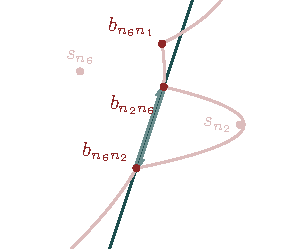
\includegraphics[width=0.5\textwidth,height=\textheight]{figures/bst/bp_edges/edges.pdf}

}

\caption{\label{fig-bst-edges}Initially the half-edges stored in each
breakpoint node are not anchored to any Voronoi vertices. When
visualizing the progression of Fortune's algorithm we can always anchor
each half-edge to the current position of the corresponding breakpoint.
This ensures that the half-edges always span at least a segment of full
Voronoi edge, shown here in dark teal.}

\end{figure}%

\subsubsection{Nearest-Neighbor Search}\label{nearest-neighbor-search}

Binary search trees feature \emph{predecessor} and \emph{successor}
operations that take any node and efficiently find the next smallest and
next largest node, respectively (Figure~\ref{fig-bst-search}). The
predecessor and successor of an arc node are always the two neighboring
breakpoint nodes, while the predecessor and success of a breakpoint node
are always the two neighboring arc nodes.

\begin{figure}

\begin{minipage}{\linewidth}

\centering{

\captionsetup{labelsep=none}
\includegraphics{figures/bst/predecessor_search/search.pdf}

}

\subcaption{\label{fig-bst-search-pred}}

\end{minipage}%
\newline
\begin{minipage}{\linewidth}

\centering{

\captionsetup{labelsep=none}
\includegraphics{figures/bst/successor_search/search.pdf}

}

\subcaption{\label{fig-bst-search-suc}}

\end{minipage}%

\caption{\label{fig-bst-search}Binary search trees are equipped with (a)
predecessor and (b) successor search operations which allow us to
navigate across neighboring objects on the beach line.}

\end{figure}%

To implement Fortune's algorithm, however, we will need to slightly
extend these nearest neighbor search operations. For example when
considering triplets of neighboring arcs for potential vertex events we
need to be able to find not just the next smallest and next largest
nodes but rather the next smallest and next largest \emph{arc} nodes.
That said, operations require just calling the standard predecessor and
successor operations twice (Figure~\ref{fig-bst-arc-search}).

\begin{figure}

\begin{minipage}{\linewidth}

\centering{

\captionsetup{labelsep=none}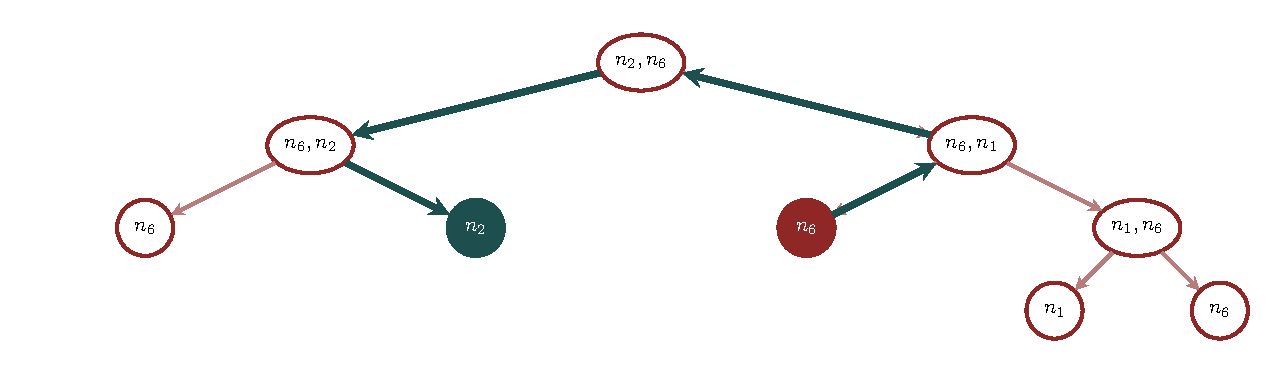
\includegraphics{figures/bst/arc_predecessor_search/search.pdf}

}

\subcaption{\label{fig-bst-arc-search-pred}}

\end{minipage}%
\newline
\begin{minipage}{\linewidth}

\centering{

\captionsetup{labelsep=none}
\includegraphics{figures/bst/arc_successor_search/search.pdf}

}

\subcaption{\label{fig-bst-arc-search-suc}}

\end{minipage}%

\caption{\label{fig-bst-arc-search}Implementing Fortune's algorithm is a
bit easier if we introduce (a) predecessor arc search and (b) successor
arc search operations which allow us to quickly construct triplets of
neighboring arcs that might spawn new Voronoi vertices.}

\end{figure}%

\subsubsection{Beach Line Search}\label{beach-line-search}

The key difference (absolutely an intentional pun) between specialized
beach line trees and generic binary search trees is that, while both are
ordered, beach line trees don't feature a traditional key. Ordering of
the nodes in a beach line tree is determined not by static key values
but rather by the relative vertical position of the arcs and breakpoints
along the corresponding beach line. As the sweep line progresses the
absolute positions change but the relative positions, and hence the
structure of the binary tree, remains invariant.

Without explicit keys beach line trees do not feature traditional key
search operations. They do, however, admit conditional positional
searches.

In particular Fortune's algorithm requires being able to find the arc in
a beach line that intersects with a particular vertical position \(y\).
To find the corresponding arc node in a beach line tree we can modify
the standard key search operation, comparing current vertical positions
at each step instead of keys (Figure~\ref{fig-bst-key-search}).

\begin{figure}

\begin{minipage}{\linewidth}

\centering{

\captionsetup{labelsep=none}
\includegraphics{figures/bst/key_search/1/bst.pdf}

}

\subcaption{\label{fig-bst-key-search1}}

\end{minipage}%
\newline
\begin{minipage}{\linewidth}

\centering{

\captionsetup{labelsep=none}
\includegraphics{figures/bst/key_search/2/bst.pdf}

}

\subcaption{\label{fig-bst-key-search2}}

\end{minipage}%
\newline
\begin{minipage}{\linewidth}

\centering{

\captionsetup{labelsep=none}
\includegraphics{figures/bst/key_search/3/bst.pdf}

}

\subcaption{\label{fig-bst-key-search3}}

\end{minipage}%

\caption{\label{fig-bst-key-search}Unlike the nodes in standard binary
search trees, the nodes in beach line binary trees are not equipped with
static keys. That said for the internal breakpoint nodes we can
dynamically compute vertical positions given the current configuration
of the beach line, which allows us to search the beach line for
positional intersections. To find the arc that intersects \(y = 3.832\)
we (a) start at the root node and then (b, c) progress down the binary
tree, evaluating current breakpoint positions as needed until we reach
an arc node.}

\end{figure}%

This operation begins by setting the current position of the sweep line,
\(S\), and then accessing the root node of the binary tree. If the root
node is an arc node then the beach line consists of a single parabola
and we're already done. Otherwise the root node is a breakpoint node and
we can compute the current vertical position of the breakpoint given
\(S\).

If the breakpoint height is larger than \(y\) then we know that the
intersecting arc is below the breakpoint in the beach line, and to the
left of the current node in the binary tree. In that case we move to the
left child of the current node. When the breakpoint height is smaller
than \(y\) then we have to move up the beach line, which is accomplished
by moving to the right child of the current node.

Regardless of which direction we take, we then just repeat these
operations until we reach a childless arc node. Because arc nodes
correspond to parabolic curves there is no single height that we can
compare to \(y\) at this point. Fortunately we no longer have to make
comparisons as the first arc node we find will always represent the arc
that intersects with \(y\).

\subsubsection{Insertion and Deletion}\label{insertion-and-deletion}

In a binary search tree the node deletion operation depends on only the
relative ordering of the nodes, and not on any explicit key values.
Consequently removing nodes is the \emph{mostly} the same operation for
beach line trees and standard binary search trees. The only subtlety is
that after removing a node we will have to update the site references in
any neighboring breakpoints.

The lack of explicit keys in a beach line tree, however, makes the
standard key insertion operation invalid. That said, Fortune's algorithm
doesn't actually require a generic key insertion. Objects are added to
the beach line in one and only one way: splitting an existing arc into
three arcs and two breakpoints. This can be compartmentalized into a
\emph{subtree insertion}.

\begin{figure}

\begin{minipage}{0.50\linewidth}

\centering{

\captionsetup{labelsep=none}
\includegraphics{figures/bst/subtree_insertion/1/bst.pdf}

}

\subcaption{\label{fig-bst-subtree-insert1}}

\end{minipage}%
%
\begin{minipage}{0.50\linewidth}

\centering{

\captionsetup{labelsep=none}
\includegraphics{figures/bst/subtree_insertion/2/bst.pdf}

}

\subcaption{\label{fig-bst-subtree-insert2}}

\end{minipage}%

\caption{\label{fig-bst-subtree-insert}In Fortune's algorithm beach line
trees are expanded through a subtree insertion operation where (a) an
arc node is replaced by a (b) subtree representing a triplet of arc
nodes and the two breakpoints between them. Note that the site
references in the initial neighboring breakpoint nodes are still
correct, and hence don't have to be updated, after the subtree
insertion.}

\end{figure}%

\subsubsection{Balancing}\label{balancing}

Number of operations needed for all of the binary tree operations we
have discussed here scales with the height of a given tree. Now the
height of most trees is logarithmic in the number of nodes, which in the
context of Fortune's algorithm is also logarithmic in the number of
sites. Consequently the tree operations usually require only a
logarithmic number of operations, and a \emph{typical} evaluation of
Fortune's algorithm will achieve an overall \(N \log N\) cost scaling.

Unfortunately the height of \emph{every} possible binary tree is not
always logarithmic in the number of nodes. In the worst case the height
of a tree can be linear in the number of nodes, pushing up the overall
cost scaling of Fortune's algorithm to quadratic.

In order to realize the optimal performance of Fortune's algorithm we
need to be able to avoid excessively tall, or \textbf{unbalanced} trees.
Conveniently this can be accomplished with the use of
\textbf{self-balancing binary trees}, in particular \textbf{red-black
trees} (Cormen et al. 2022). These data structures modify the standard
insertion and deletion operations to ensure that nodes are
well-distributed across the entire tree. With a little bit of effort we
can adapt these balanced operations to beach line trees, which then
allows us to achieve optimal performance when implementing Fortune's
algorithm.

\subsection{The Event Queue}\label{the-event-queue}

The event queue in Fortune's algorithm can be efficiently implemented
with a \textbf{priority queue} data structure (Cormen et al. 2022).
Priority queues are equipped with an operation for ``popping'' the next
element off the queue as well as operations for inserting and deleting
elements while maintaining the overall order of the event queue.

To implement Fortune's algorithm we'll need to consider two types of
events. Vertex events contain the position of the sweep line where an
arc will collapse and a reference to that arc. Site events, on the other
hand, contain the position where sweep line will encounter a new site as
well as a reference to that site.

\subsection{Event Processing}\label{event-processing}

Fortune's algorithm proceeds by popping the next event off of the event
queue, using that event to advanced the sweep line and beach line, and
then updating the Voronoi graph as necessary. With doubly-connected
event queues, binary search trees, and their operations processing each
event is relatively straightforward.

\subsection{Processing Vertex Events}\label{processing-vertex-events}

The first step when processing a new vertex event is to remove any other
vertex events that will become invalid after we remove the collapsing
arc. This can be done efficiently by using the arc predecessor and arc
successor operations of the beach line tree to find the neighboring
arcs, and then remove any vertex events referenced in those arcs.

Next we manage the expansion of the Voronoi graph. We begin by adding a
new vertex to the doubly-connected edge list at the point where the arc
collapses and the neighboring breakpoints intersect.

Then we have to deal with the Voronoi edges. We create a new half-edge
originating at the new vertex and its twin that, for the moment, is left
unanchored (Figure~\ref{fig-vertex-event-edges}). Lastly we link up the
previous and next references between these two new half-edges, the two
half-edges in the neighboring breakpoints, and their twins
(Figure~\ref{fig-vertex-event-edge-connections}).

\begin{figure}

\begin{minipage}{0.50\linewidth}

\centering{

\captionsetup{labelsep=none}
\includegraphics{figures/fortune/edges/vertex/1/edges.pdf}

}

\subcaption{\label{fig-vertex-event-edges1}}

\end{minipage}%
%
\begin{minipage}{0.50\linewidth}

\centering{

\captionsetup{labelsep=none}
\includegraphics{figures/fortune/edges/vertex/2/edges.pdf}

}

\subcaption{\label{fig-vertex-event-edges2}}

\end{minipage}%
\newline
\begin{minipage}{0.25\linewidth}
~\end{minipage}%
%
\begin{minipage}{0.50\linewidth}

\centering{

\captionsetup{labelsep=none}
\includegraphics{figures/fortune/edges/vertex/3/edges.pdf}

}

\subcaption{\label{fig-vertex-event-edges3}}

\end{minipage}%
%
\begin{minipage}{0.25\linewidth}
~\end{minipage}%

\caption{\label{fig-vertex-event-edges}Vertex events require substantial
updates to the half-edges of the Voronoi graph. (a) The breakpoints that
merge in a vertex event contain references to two half-edges, here
\texttt{he1} and \texttt{he3}. (b) When processing a vertex event we
delete these references. (c) Then we create two new half-edges, one of
which is referenced by the new vertex, here \texttt{he5}, and one of
which is referenced by the new breakpoint, here \texttt{he6}.}

\end{figure}%

\begin{figure}

\centering{


\includegraphics[width=0.5\textwidth,height=\textheight]{figures/fortune/edges/connections/edges.pdf}

}

\caption{\label{fig-vertex-event-edge-connections}The trickiest part of
processing a vertex event is making sure that the four existing
half-edges and the two new half-edges all properly reference each other.
These references ultimately form the skeleton of the Voronoi graph.}

\end{figure}%

Now we're ready to remove the collapsing arc. This requires removing the
corresponding arc node as well as one of its neighboring breakpoint
nodes, rebalancing the binary search tree after each removal
(Figure~\ref{fig-vertex-event-deletion}). Which breakpoint node we
remove is a matter of convention, but to avoid any ambiguity I will
maintain a convention where we always remove the smaller breakpoint.

\begin{figure}

\begin{minipage}{\linewidth}

\centering{

\captionsetup{labelsep=none}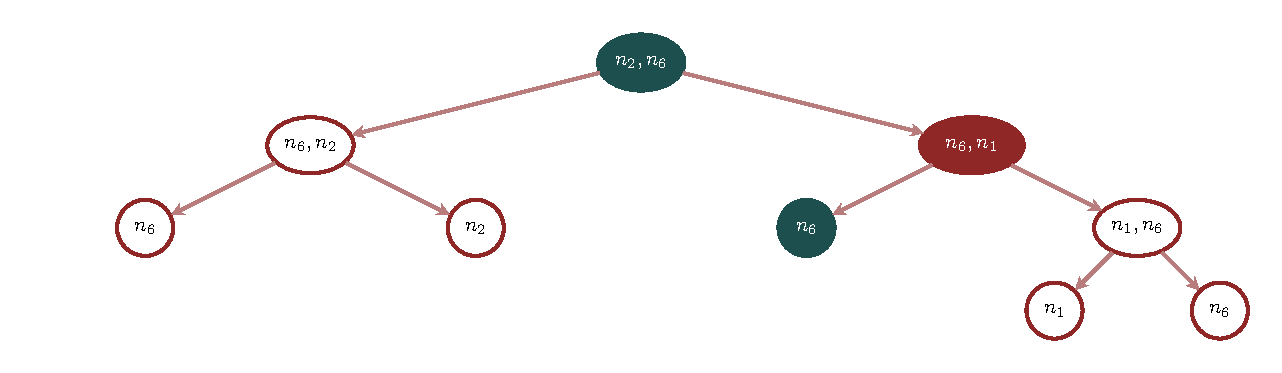
\includegraphics{figures/bst/deletion/1/deletion.pdf}

}

\subcaption{\label{fig-vertex-event-deletion1}}

\end{minipage}%
\newline
\begin{minipage}{\linewidth}

\centering{

\captionsetup{labelsep=none}
\includegraphics{figures/bst/deletion/2/deletion.pdf}

}

\subcaption{\label{fig-vertex-event-deletion2}}

\end{minipage}%
\newline
\begin{minipage}{\linewidth}

\centering{

\captionsetup{labelsep=none}
\includegraphics{figures/bst/deletion/3/deletion.pdf}

}

\subcaption{\label{fig-vertex-event-deletion3}}

\end{minipage}%

\caption{\label{fig-vertex-event-deletion}(a, b) Removing an arc from a
beach line requires deleting two nodes from the corresponding binary
tree, a leaf node for the arc itself and an internal node for one of the
neighboring breakpoints. Which breakpoint we remove is a matter of
convention. (c) After removing the two nodes from the binary tree we
need to update the site information in the remaining breakpoint node.
Here the left site has to be updated from \(n_{6}\) to \(n_{2}\).}

\end{figure}%

At this point the remaining breakpoint node, the larger breakpoint in my
chosen convention, needs to be updated. Firstly its left site needs to
be updated to the site that generates its new left neighboring arc; this
new neighbor can be accessed by calling the predecessor operation on the
updated tree. Secondly we need to set its half-edge references to the
new twin half-edge that we just created.

Lastly there are two new triplets of neighboring arcs that we have to
check for possible new vertex events. We can efficiently access these
arcs by repeatedly using the arc predecessor and arc successor
operations

\subsubsection{Processing Site Events}\label{processing-site-events}

Because site events do not update the Voronoi diagram they are a little
bit easier to process.

First things first we have to find the arc that intersects with the
height of the new site by searching through the beach line tree. Because
splitting this arc will invalidate any existing vertex event centered on
it, we have to remove any corresponding vertex event from the event
queue.

In order to incorporate the new site into the beach line we have to
apply the subtree insertion operation on the intersecting node, replace
it with a subtree that includes two arc nodes associated with the
original site, one arc node associated with the new site, and two
interior breakpoint nodes separating them. When working with a balanced
binary tree we also have to make sure that this insertion operation
properly rebalances the updated tree.

The two new breakpoint nodes are then filled with two new half-edges
that are twinned to each other (Figure~\ref{fig-site-event-edges}). One
half-edge faces the old site and the other faces the face the new site.

\begin{figure}

\centering{


\includegraphics[width=0.5\textwidth,height=\textheight]{figures/fortune/edges/site/edges.pdf}

}

\caption{\label{fig-site-event-edges}The introduction of a new site
splits an existing arc on the beach line into three arcs separated by
two new breakpoints. This also creates two new half-edges in the Voronoi
graph that are twinned with each other. A reference to each of these
half-edges is stored in one of the two new breakpoint nodes that are
inserted into the beach line tree. Here a reference to the half-edge
\texttt{he1} is stored in the breakpoint node \texttt{(n1,\ n2)} while a
reference to \texttt{he2} is stored in the breakpoint node
\texttt{(n2,\ n1)}.}

\end{figure}%

Finally we have to consider potential new vertex events that.
Incorporating the new site creates up to two new triplets of neighboring
arcs that might generate new vertex events. Fortunately the arc nodes in
these new triplets are once again readily accessed with the arc
predecessor and arc successor beach line operations.

\section{Clean Up}\label{clean-up-1}

Once the event queue is exhausted we are left with a doubly-connected
edge list that contains all of the information about the Voronoi graph,
and hence the Voronoi diagram.

At this point the binary search tree implementing the beach line will
\emph{not} be empty. The remaining breakpoint nodes all contain
half-edges with unbounded origins. If we want to visualize the Voronoi
graph neatly then we'll need to anchor these dangling edges by creating
a bounding box and then adding a pseudo-vector to the doubly-connected
edge list for the intersection of each dangling half-edge with the
bounding box.

\section{Demonstration}\label{demonstration}

To put all of this discussion into practice let's work through a full
implementation of Fortune's algorithm in \texttt{R}. To be honest
\texttt{R} is at best an awkward language for this application, which is
much more natural in languages that are more friendly to object-oriented
programming.

Here I get by with \texttt{R6} classes (Chang 2025), but we'll have to
suffer with some of its clumsy interactions with base \texttt{R}
graphics. At least using \texttt{R6} classes gets us pass-by-reference
semantics for class instances instead of \texttt{R}'s usual
call-by-need/lazy evaluation semantics.

\begin{Shaded}
\begin{Highlighting}[]
\FunctionTok{library}\NormalTok{(R6)}
\end{Highlighting}
\end{Shaded}

\begin{verbatim}
Warning: package 'R6' was built under R version 4.3.3
\end{verbatim}

Speaking of graphics, we'll start with some graphics settings.

\begin{Shaded}
\begin{Highlighting}[]
\FunctionTok{par}\NormalTok{(}\AttributeTok{family=}\StringTok{"serif"}\NormalTok{, }\AttributeTok{las=}\DecValTok{1}\NormalTok{, }\AttributeTok{bty=}\StringTok{"l"}\NormalTok{,}
    \AttributeTok{cex.axis=}\DecValTok{1}\NormalTok{, }\AttributeTok{cex.lab=}\DecValTok{1}\NormalTok{, }\AttributeTok{cex.main=}\DecValTok{1}\NormalTok{,}
    \AttributeTok{xaxs=}\StringTok{"i"}\NormalTok{, }\AttributeTok{yaxs=}\StringTok{"i"}\NormalTok{, }\AttributeTok{mar =} \FunctionTok{c}\NormalTok{(}\DecValTok{5}\NormalTok{, }\DecValTok{5}\NormalTok{, }\DecValTok{3}\NormalTok{, }\DecValTok{1}\NormalTok{))}

\NormalTok{c\_light }\OtherTok{\textless{}{-}} \FunctionTok{c}\NormalTok{(}\StringTok{"\#DCBCBC"}\NormalTok{)}
\NormalTok{c\_light\_highlight }\OtherTok{\textless{}{-}} \FunctionTok{c}\NormalTok{(}\StringTok{"\#C79999"}\NormalTok{)}
\NormalTok{c\_mid }\OtherTok{\textless{}{-}} \FunctionTok{c}\NormalTok{(}\StringTok{"\#B97C7C"}\NormalTok{)}
\NormalTok{c\_mid\_highlight }\OtherTok{\textless{}{-}} \FunctionTok{c}\NormalTok{(}\StringTok{"\#A25050"}\NormalTok{)}
\NormalTok{c\_dark }\OtherTok{\textless{}{-}} \FunctionTok{c}\NormalTok{(}\StringTok{"\#8F2727"}\NormalTok{)}
\NormalTok{c\_dark\_highlight }\OtherTok{\textless{}{-}} \FunctionTok{c}\NormalTok{(}\StringTok{"\#7C0000"}\NormalTok{)}

\NormalTok{c\_light\_teal }\OtherTok{\textless{}{-}} \FunctionTok{c}\NormalTok{(}\StringTok{"\#6B8E8E"}\NormalTok{)}
\NormalTok{c\_mid\_teal }\OtherTok{\textless{}{-}} \FunctionTok{c}\NormalTok{(}\StringTok{"\#487575"}\NormalTok{)}
\NormalTok{c\_dark\_teal }\OtherTok{\textless{}{-}} \FunctionTok{c}\NormalTok{(}\StringTok{"\#1D4F4F"}\NormalTok{)}
\end{Highlighting}
\end{Shaded}

\subsection{Beach Line}\label{beach-line}

To define a beach line we'll first need nodes.

This class implements both breakpoint and arc nodes by including the
satellite data for each and using only one type of data at a time. In
particular the variables \texttt{site} and \texttt{scheduled\_vertex}
are used for only arc nodes while \texttt{site\_left},
\texttt{site\_right}, and \texttt{he} are used for only breakpoint
nodes. Note that the site variables are integer indices which will be
used to access site information from global arrays.

The variable \texttt{red} denotes the coloring of the node which is used
for balancing binary trees.

\begin{Shaded}
\begin{Highlighting}[]
\NormalTok{node }\OtherTok{\textless{}{-}} \FunctionTok{R6Class}\NormalTok{(}\StringTok{"node"}\NormalTok{,}
                \AttributeTok{public =} \FunctionTok{list}\NormalTok{(}
                  \AttributeTok{site =} \ConstantTok{NULL}\NormalTok{,}
                  \AttributeTok{scheduled\_vertex =} \ConstantTok{NULL}\NormalTok{,}
                  \AttributeTok{site\_left =} \ConstantTok{NULL}\NormalTok{,}
                  \AttributeTok{site\_right =} \ConstantTok{NULL}\NormalTok{,}
                  \AttributeTok{he =} \ConstantTok{NULL}\NormalTok{,}
                  \AttributeTok{parent =} \ConstantTok{NULL}\NormalTok{,}
                  \AttributeTok{left =} \ConstantTok{NULL}\NormalTok{,}
                  \AttributeTok{right =} \ConstantTok{NULL}\NormalTok{,}
                  \AttributeTok{red =} \ConstantTok{FALSE}\NormalTok{,}
                  \AttributeTok{id =} \ConstantTok{NULL}\NormalTok{,}
                  \AttributeTok{initialize =} \ControlFlowTok{function}\NormalTok{(beachline) \{}
                    \ControlFlowTok{if}\NormalTok{ (}\FunctionTok{is.integer}\NormalTok{(beachline)) \{}
\NormalTok{                      self}\SpecialCharTok{$}\NormalTok{id }\OtherTok{\textless{}{-}}\NormalTok{ beachline}
\NormalTok{                    \} }\ControlFlowTok{else}\NormalTok{ \{}
\NormalTok{                      self}\SpecialCharTok{$}\NormalTok{parent }\OtherTok{\textless{}{-}}\NormalTok{ beachline}\SpecialCharTok{$}\NormalTok{nil}
\NormalTok{                      self}\SpecialCharTok{$}\NormalTok{left }\OtherTok{\textless{}{-}}\NormalTok{ beachline}\SpecialCharTok{$}\NormalTok{nil}
\NormalTok{                      self}\SpecialCharTok{$}\NormalTok{right }\OtherTok{\textless{}{-}}\NormalTok{ beachline}\SpecialCharTok{$}\NormalTok{nil}

\NormalTok{                      beachline}\SpecialCharTok{$}\NormalTok{last\_node\_id }\OtherTok{\textless{}{-}}\NormalTok{ beachline}\SpecialCharTok{$}\NormalTok{last\_node\_id }\SpecialCharTok{+} \DecValTok{1}
\NormalTok{                      self}\SpecialCharTok{$}\NormalTok{id }\OtherTok{\textless{}{-}}\NormalTok{ beachline}\SpecialCharTok{$}\NormalTok{last\_node\_id}
\NormalTok{                    \}}
\NormalTok{                  \}}
\NormalTok{                )}
\NormalTok{)}
\end{Highlighting}
\end{Shaded}

The \texttt{id} variable allows us to determine if two \texttt{node}
instances refer to the same object. In many programming languages this
is done by directly comparing memory addresses, but \texttt{R6} classes
don't seem to play will with memory.

\begin{Shaded}
\begin{Highlighting}[]
\StringTok{\textasciigrave{}}\AttributeTok{==.node}\StringTok{\textasciigrave{}} \OtherTok{=} \ControlFlowTok{function}\NormalTok{(x, y) \{ x}\SpecialCharTok{$}\NormalTok{id }\SpecialCharTok{==}\NormalTok{ y}\SpecialCharTok{$}\NormalTok{id \}}
\StringTok{\textasciigrave{}}\AttributeTok{!=.node}\StringTok{\textasciigrave{}} \OtherTok{=} \ControlFlowTok{function}\NormalTok{(x, y) \{ x}\SpecialCharTok{$}\NormalTok{id }\SpecialCharTok{!=}\NormalTok{ y}\SpecialCharTok{$}\NormalTok{id \}}
\end{Highlighting}
\end{Shaded}

An actual beach line tree is defined by a root node. Here we'll be using
a self-balancing red-black binary tree which uses the coloring of the
nodes to limit the height of any given tree. Red-black binary trees
requires a dedicated null, or nil, node.

\begin{Shaded}
\begin{Highlighting}[]
\NormalTok{beachline }\OtherTok{\textless{}{-}} \FunctionTok{R6Class}\NormalTok{(}\StringTok{"beachline"}\NormalTok{,}
                     \AttributeTok{public =} \FunctionTok{list}\NormalTok{(}
                       \AttributeTok{nil =} \ConstantTok{NULL}\NormalTok{,}
                       \AttributeTok{root =} \ConstantTok{NULL}\NormalTok{,}
                       \AttributeTok{last\_node\_id =} \ConstantTok{NULL}\NormalTok{,}
                       \AttributeTok{last\_half\_edge\_id =} \ConstantTok{NULL}\NormalTok{,}
                       \AttributeTok{initialize =} \ControlFlowTok{function}\NormalTok{() \{}
\NormalTok{                         self}\SpecialCharTok{$}\NormalTok{nil }\OtherTok{\textless{}{-}}\NormalTok{ node}\SpecialCharTok{$}\FunctionTok{new}\NormalTok{(}\FunctionTok{as.integer}\NormalTok{(}\DecValTok{0}\NormalTok{))}
\NormalTok{                         self}\SpecialCharTok{$}\NormalTok{root }\OtherTok{\textless{}{-}}\NormalTok{ self}\SpecialCharTok{$}\NormalTok{nil}
\NormalTok{                         self}\SpecialCharTok{$}\NormalTok{last\_node\_id }\OtherTok{\textless{}{-}} \FunctionTok{as.integer}\NormalTok{(}\DecValTok{1}\NormalTok{)}
\NormalTok{                         self}\SpecialCharTok{$}\NormalTok{last\_half\_edge\_id }\OtherTok{\textless{}{-}} \FunctionTok{as.integer}\NormalTok{(}\DecValTok{1}\NormalTok{)}
\NormalTok{                       \}}
\NormalTok{                     ))}
\end{Highlighting}
\end{Shaded}

The \texttt{beachline} class also gives us a place to keep track of the
node indices, as well as half-edge indices that we'll use later.

\subsubsection{Black-Red Binary Tree
Operations}\label{black-red-binary-tree-operations}

The \texttt{insert\_fixup} function rebalances a binary tree after we
add the node \texttt{z} to the tree.

\begin{Shaded}
\begin{Highlighting}[]
\NormalTok{beachline}\SpecialCharTok{$}\FunctionTok{set}\NormalTok{(}\StringTok{"private"}\NormalTok{, }\StringTok{"left\_rotate"}\NormalTok{,}
\ControlFlowTok{function}\NormalTok{(x) \{}
  \ControlFlowTok{if}\NormalTok{ (x}\SpecialCharTok{$}\NormalTok{right }\SpecialCharTok{==}\NormalTok{ self}\SpecialCharTok{$}\NormalTok{nil)}
    \FunctionTok{return}\NormalTok{()}

\NormalTok{  y }\OtherTok{\textless{}{-}}\NormalTok{ x}\SpecialCharTok{$}\NormalTok{right}
\NormalTok{  x}\SpecialCharTok{$}\NormalTok{right }\OtherTok{\textless{}{-}}\NormalTok{ y}\SpecialCharTok{$}\NormalTok{left}

  \ControlFlowTok{if}\NormalTok{ (y}\SpecialCharTok{$}\NormalTok{left }\SpecialCharTok{!=}\NormalTok{ self}\SpecialCharTok{$}\NormalTok{nil)}
\NormalTok{    y}\SpecialCharTok{$}\NormalTok{left}\SpecialCharTok{$}\NormalTok{parent }\OtherTok{\textless{}{-}}\NormalTok{ x}

\NormalTok{  y}\SpecialCharTok{$}\NormalTok{parent }\OtherTok{\textless{}{-}}\NormalTok{ x}\SpecialCharTok{$}\NormalTok{parent}

  \ControlFlowTok{if}\NormalTok{ (x}\SpecialCharTok{$}\NormalTok{parent }\SpecialCharTok{==}\NormalTok{ self}\SpecialCharTok{$}\NormalTok{nil) \{}
\NormalTok{    self}\SpecialCharTok{$}\NormalTok{root }\OtherTok{\textless{}{-}}\NormalTok{ y}
\NormalTok{  \} }\ControlFlowTok{else}\NormalTok{ \{}
    \ControlFlowTok{if}\NormalTok{ (x}\SpecialCharTok{$}\NormalTok{parent}\SpecialCharTok{$}\NormalTok{left }\SpecialCharTok{==}\NormalTok{ x)}
\NormalTok{      x}\SpecialCharTok{$}\NormalTok{parent}\SpecialCharTok{$}\NormalTok{left }\OtherTok{\textless{}{-}}\NormalTok{ y}
    \ControlFlowTok{else}
\NormalTok{      x}\SpecialCharTok{$}\NormalTok{parent}\SpecialCharTok{$}\NormalTok{right }\OtherTok{\textless{}{-}}\NormalTok{ y}
\NormalTok{  \}}

\NormalTok{  y}\SpecialCharTok{$}\NormalTok{left }\OtherTok{\textless{}{-}}\NormalTok{ x}
\NormalTok{  x}\SpecialCharTok{$}\NormalTok{parent }\OtherTok{\textless{}{-}}\NormalTok{ y}
\NormalTok{\})}
\end{Highlighting}
\end{Shaded}

\begin{Shaded}
\begin{Highlighting}[]
\NormalTok{beachline}\SpecialCharTok{$}\FunctionTok{set}\NormalTok{(}\StringTok{"private"}\NormalTok{, }\StringTok{"right\_rotate"}\NormalTok{,}
\ControlFlowTok{function}\NormalTok{(x) \{}
  \ControlFlowTok{if}\NormalTok{ (x}\SpecialCharTok{$}\NormalTok{left }\SpecialCharTok{==}\NormalTok{ self}\SpecialCharTok{$}\NormalTok{nil)}
    \FunctionTok{return}\NormalTok{()}

\NormalTok{  y }\OtherTok{\textless{}{-}}\NormalTok{ x}\SpecialCharTok{$}\NormalTok{left}
\NormalTok{  x}\SpecialCharTok{$}\NormalTok{left }\OtherTok{\textless{}{-}}\NormalTok{ y}\SpecialCharTok{$}\NormalTok{right}

  \ControlFlowTok{if}\NormalTok{ (y}\SpecialCharTok{$}\NormalTok{right }\SpecialCharTok{!=}\NormalTok{ self}\SpecialCharTok{$}\NormalTok{nil)}
\NormalTok{    y}\SpecialCharTok{$}\NormalTok{right}\SpecialCharTok{$}\NormalTok{parent }\OtherTok{\textless{}{-}}\NormalTok{ x}

\NormalTok{  y}\SpecialCharTok{$}\NormalTok{parent }\OtherTok{\textless{}{-}}\NormalTok{ x}\SpecialCharTok{$}\NormalTok{parent}

  \ControlFlowTok{if}\NormalTok{ (x}\SpecialCharTok{$}\NormalTok{parent }\SpecialCharTok{==}\NormalTok{ self}\SpecialCharTok{$}\NormalTok{nil) \{}
\NormalTok{    self}\SpecialCharTok{$}\NormalTok{root }\OtherTok{\textless{}{-}}\NormalTok{ y}
\NormalTok{  \} }\ControlFlowTok{else}\NormalTok{ \{}
    \ControlFlowTok{if}\NormalTok{ (x}\SpecialCharTok{$}\NormalTok{parent}\SpecialCharTok{$}\NormalTok{right }\SpecialCharTok{==}\NormalTok{ x)}
\NormalTok{      x}\SpecialCharTok{$}\NormalTok{parent}\SpecialCharTok{$}\NormalTok{right }\OtherTok{\textless{}{-}}\NormalTok{ y}
    \ControlFlowTok{else}
\NormalTok{      x}\SpecialCharTok{$}\NormalTok{parent}\SpecialCharTok{$}\NormalTok{left }\OtherTok{\textless{}{-}}\NormalTok{ y}
\NormalTok{  \}}

\NormalTok{  y}\SpecialCharTok{$}\NormalTok{right }\OtherTok{\textless{}{-}}\NormalTok{ x}
\NormalTok{  x}\SpecialCharTok{$}\NormalTok{parent }\OtherTok{\textless{}{-}}\NormalTok{ y}
\NormalTok{\})}
\end{Highlighting}
\end{Shaded}

\begin{Shaded}
\begin{Highlighting}[]
\NormalTok{beachline}\SpecialCharTok{$}\FunctionTok{set}\NormalTok{(}\StringTok{"private"}\NormalTok{, }\StringTok{"insert\_fixup"}\NormalTok{,}
\ControlFlowTok{function}\NormalTok{(z) \{}
  \ControlFlowTok{while}\NormalTok{ (z}\SpecialCharTok{$}\NormalTok{parent}\SpecialCharTok{$}\NormalTok{red) \{}
    \ControlFlowTok{if}\NormalTok{ (z}\SpecialCharTok{$}\NormalTok{parent }\SpecialCharTok{==}\NormalTok{ z}\SpecialCharTok{$}\NormalTok{parent}\SpecialCharTok{$}\NormalTok{parent}\SpecialCharTok{$}\NormalTok{left) \{}
\NormalTok{      y }\OtherTok{\textless{}{-}}\NormalTok{ z}\SpecialCharTok{$}\NormalTok{parent}\SpecialCharTok{$}\NormalTok{parent}\SpecialCharTok{$}\NormalTok{right}
      \ControlFlowTok{if}\NormalTok{ (y}\SpecialCharTok{$}\NormalTok{red) \{}
\NormalTok{        z}\SpecialCharTok{$}\NormalTok{parent}\SpecialCharTok{$}\NormalTok{red }\OtherTok{\textless{}{-}} \ConstantTok{FALSE}
\NormalTok{        y}\SpecialCharTok{$}\NormalTok{red }\OtherTok{\textless{}{-}} \ConstantTok{FALSE}
\NormalTok{        z}\SpecialCharTok{$}\NormalTok{parent}\SpecialCharTok{$}\NormalTok{parent}\SpecialCharTok{$}\NormalTok{red }\OtherTok{\textless{}{-}} \ConstantTok{TRUE}
\NormalTok{        z }\OtherTok{\textless{}{-}}\NormalTok{ z}\SpecialCharTok{$}\NormalTok{parent}\SpecialCharTok{$}\NormalTok{parent}
\NormalTok{      \} }\ControlFlowTok{else}\NormalTok{ \{}
        \ControlFlowTok{if}\NormalTok{ (z }\SpecialCharTok{==}\NormalTok{ z}\SpecialCharTok{$}\NormalTok{parent}\SpecialCharTok{$}\NormalTok{right) \{}
\NormalTok{          z }\OtherTok{\textless{}{-}}\NormalTok{ z}\SpecialCharTok{$}\NormalTok{parent}
\NormalTok{          private}\SpecialCharTok{$}\FunctionTok{left\_rotate}\NormalTok{(z)}
\NormalTok{        \}}
\NormalTok{        z}\SpecialCharTok{$}\NormalTok{parent}\SpecialCharTok{$}\NormalTok{red }\OtherTok{\textless{}{-}} \ConstantTok{FALSE}
\NormalTok{        z}\SpecialCharTok{$}\NormalTok{parent}\SpecialCharTok{$}\NormalTok{parent}\SpecialCharTok{$}\NormalTok{red }\OtherTok{\textless{}{-}} \ConstantTok{TRUE}
\NormalTok{        private}\SpecialCharTok{$}\FunctionTok{right\_rotate}\NormalTok{(z}\SpecialCharTok{$}\NormalTok{parent}\SpecialCharTok{$}\NormalTok{parent)}
\NormalTok{      \}}
\NormalTok{    \} }\ControlFlowTok{else}\NormalTok{ \{}
\NormalTok{      y }\OtherTok{\textless{}{-}}\NormalTok{ z}\SpecialCharTok{$}\NormalTok{parent}\SpecialCharTok{$}\NormalTok{parent}\SpecialCharTok{$}\NormalTok{left}

      \ControlFlowTok{if}\NormalTok{ (y}\SpecialCharTok{$}\NormalTok{red) \{}
\NormalTok{        z}\SpecialCharTok{$}\NormalTok{parent}\SpecialCharTok{$}\NormalTok{red }\OtherTok{\textless{}{-}} \ConstantTok{FALSE}
\NormalTok{        y}\SpecialCharTok{$}\NormalTok{red }\OtherTok{\textless{}{-}} \ConstantTok{FALSE}
\NormalTok{        z}\SpecialCharTok{$}\NormalTok{parent}\SpecialCharTok{$}\NormalTok{parent}\SpecialCharTok{$}\NormalTok{red }\OtherTok{\textless{}{-}} \ConstantTok{TRUE}
\NormalTok{        z }\OtherTok{\textless{}{-}}\NormalTok{ z}\SpecialCharTok{$}\NormalTok{parent}\SpecialCharTok{$}\NormalTok{parent}
\NormalTok{      \} }\ControlFlowTok{else}\NormalTok{ \{}
        \ControlFlowTok{if}\NormalTok{ (z }\SpecialCharTok{==}\NormalTok{ z}\SpecialCharTok{$}\NormalTok{parent}\SpecialCharTok{$}\NormalTok{left) \{}
\NormalTok{          z }\OtherTok{\textless{}{-}}\NormalTok{ z}\SpecialCharTok{$}\NormalTok{parent}
\NormalTok{          private}\SpecialCharTok{$}\FunctionTok{right\_rotate}\NormalTok{(z)}
\NormalTok{        \}}
\NormalTok{        z}\SpecialCharTok{$}\NormalTok{parent}\SpecialCharTok{$}\NormalTok{red }\OtherTok{\textless{}{-}} \ConstantTok{FALSE}
\NormalTok{        z}\SpecialCharTok{$}\NormalTok{parent}\SpecialCharTok{$}\NormalTok{parent}\SpecialCharTok{$}\NormalTok{red }\OtherTok{\textless{}{-}} \ConstantTok{TRUE}
\NormalTok{        private}\SpecialCharTok{$}\FunctionTok{left\_rotate}\NormalTok{(z}\SpecialCharTok{$}\NormalTok{parent}\SpecialCharTok{$}\NormalTok{parent)}
\NormalTok{      \}}
\NormalTok{    \}}
\NormalTok{  \}}
\NormalTok{  self}\SpecialCharTok{$}\NormalTok{root}\SpecialCharTok{$}\NormalTok{red }\OtherTok{\textless{}{-}} \ConstantTok{FALSE}
\NormalTok{\})}
\end{Highlighting}
\end{Shaded}

Deleting a node from a red-black tree takes some care. To properly
remove a node we'll need to be able to calculate the boundaries of
subtrees.

\begin{Shaded}
\begin{Highlighting}[]
\NormalTok{beachline}\SpecialCharTok{$}\FunctionTok{set}\NormalTok{(}\StringTok{"public"}\NormalTok{, }\StringTok{"min"}\NormalTok{,}
\ControlFlowTok{function}\NormalTok{(x) \{}
  \ControlFlowTok{if}\NormalTok{ (x }\SpecialCharTok{==}\NormalTok{ self}\SpecialCharTok{$}\NormalTok{nil)}
    \FunctionTok{return}\NormalTok{(self}\SpecialCharTok{$}\NormalTok{nil)}
  \ControlFlowTok{while}\NormalTok{ (x}\SpecialCharTok{$}\NormalTok{left }\SpecialCharTok{!=}\NormalTok{ self}\SpecialCharTok{$}\NormalTok{nil)}
\NormalTok{    x }\OtherTok{\textless{}{-}}\NormalTok{ x}\SpecialCharTok{$}\NormalTok{left}
\NormalTok{  x}
\NormalTok{\})}
\end{Highlighting}
\end{Shaded}

\begin{Shaded}
\begin{Highlighting}[]
\NormalTok{beachline}\SpecialCharTok{$}\FunctionTok{set}\NormalTok{(}\StringTok{"public"}\NormalTok{, }\StringTok{"max"}\NormalTok{,}
\ControlFlowTok{function}\NormalTok{(x) \{}
  \ControlFlowTok{if}\NormalTok{ (x }\SpecialCharTok{==}\NormalTok{ self}\SpecialCharTok{$}\NormalTok{nil)}
    \FunctionTok{return}\NormalTok{(self}\SpecialCharTok{$}\NormalTok{nil)}
  \ControlFlowTok{while}\NormalTok{ (x}\SpecialCharTok{$}\NormalTok{right }\SpecialCharTok{!=}\NormalTok{ self}\SpecialCharTok{$}\NormalTok{nil)}
\NormalTok{    x }\OtherTok{\textless{}{-}}\NormalTok{ x}\SpecialCharTok{$}\NormalTok{right}
\NormalTok{  x}
\NormalTok{\})}
\end{Highlighting}
\end{Shaded}

Then we'll need to carefully rebalance the tree.

\begin{Shaded}
\begin{Highlighting}[]
\NormalTok{beachline}\SpecialCharTok{$}\FunctionTok{set}\NormalTok{(}\StringTok{"private"}\NormalTok{, }\StringTok{"transplant"}\NormalTok{,}
\ControlFlowTok{function}\NormalTok{(u, v) \{}
  \ControlFlowTok{if}\NormalTok{ (u}\SpecialCharTok{$}\NormalTok{parent }\SpecialCharTok{==}\NormalTok{ self}\SpecialCharTok{$}\NormalTok{nil) \{}
\NormalTok{    self}\SpecialCharTok{$}\NormalTok{root }\OtherTok{\textless{}{-}}\NormalTok{ v}
\NormalTok{  \} }\ControlFlowTok{else}\NormalTok{ \{}
    \ControlFlowTok{if}\NormalTok{ (u }\SpecialCharTok{==}\NormalTok{ u}\SpecialCharTok{$}\NormalTok{parent}\SpecialCharTok{$}\NormalTok{left) \{}
\NormalTok{      u}\SpecialCharTok{$}\NormalTok{parent}\SpecialCharTok{$}\NormalTok{left }\OtherTok{\textless{}{-}}\NormalTok{ v}
\NormalTok{    \} }\ControlFlowTok{else}\NormalTok{ \{}
\NormalTok{      u}\SpecialCharTok{$}\NormalTok{parent}\SpecialCharTok{$}\NormalTok{right }\OtherTok{\textless{}{-}}\NormalTok{ v}
\NormalTok{    \}}
\NormalTok{  \}}
\NormalTok{  v}\SpecialCharTok{$}\NormalTok{parent }\OtherTok{\textless{}{-}}\NormalTok{ u}\SpecialCharTok{$}\NormalTok{parent}
\NormalTok{\})}
\end{Highlighting}
\end{Shaded}

\begin{Shaded}
\begin{Highlighting}[]
\NormalTok{beachline}\SpecialCharTok{$}\FunctionTok{set}\NormalTok{(}\StringTok{"private"}\NormalTok{, }\StringTok{"delete\_fixup"}\NormalTok{,}
\ControlFlowTok{function}\NormalTok{(x) \{}
  \ControlFlowTok{while}\NormalTok{ (x }\SpecialCharTok{!=}\NormalTok{ self}\SpecialCharTok{$}\NormalTok{root }\SpecialCharTok{\&\&} \SpecialCharTok{!}\NormalTok{x}\SpecialCharTok{$}\NormalTok{red) \{}
    \ControlFlowTok{if}\NormalTok{ (x }\SpecialCharTok{==}\NormalTok{ x}\SpecialCharTok{$}\NormalTok{parent}\SpecialCharTok{$}\NormalTok{left) \{}
\NormalTok{      w }\OtherTok{\textless{}{-}}\NormalTok{ x}\SpecialCharTok{$}\NormalTok{parent}\SpecialCharTok{$}\NormalTok{right}

      \ControlFlowTok{if}\NormalTok{ (w}\SpecialCharTok{$}\NormalTok{red) \{}
\NormalTok{        w}\SpecialCharTok{$}\NormalTok{red }\OtherTok{\textless{}{-}} \ConstantTok{FALSE}
\NormalTok{        x}\SpecialCharTok{$}\NormalTok{parent}\SpecialCharTok{$}\NormalTok{red }\OtherTok{\textless{}{-}} \ConstantTok{TRUE}
\NormalTok{        private}\SpecialCharTok{$}\FunctionTok{left\_rotate}\NormalTok{(x}\SpecialCharTok{$}\NormalTok{parent)}
\NormalTok{        w }\OtherTok{\textless{}{-}}\NormalTok{ x}\SpecialCharTok{$}\NormalTok{parent}\SpecialCharTok{$}\NormalTok{right}
\NormalTok{      \}}

      \ControlFlowTok{if}\NormalTok{ (}\SpecialCharTok{!}\NormalTok{w}\SpecialCharTok{$}\NormalTok{left}\SpecialCharTok{$}\NormalTok{red }\SpecialCharTok{\&\&} \SpecialCharTok{!}\NormalTok{w}\SpecialCharTok{$}\NormalTok{right}\SpecialCharTok{$}\NormalTok{red) \{}
\NormalTok{        w}\SpecialCharTok{$}\NormalTok{red }\OtherTok{\textless{}{-}} \ConstantTok{TRUE}
\NormalTok{        x }\OtherTok{\textless{}{-}}\NormalTok{ x}\SpecialCharTok{$}\NormalTok{parent}
\NormalTok{      \} }\ControlFlowTok{else}\NormalTok{ \{}
        \ControlFlowTok{if}\NormalTok{ (}\SpecialCharTok{!}\NormalTok{w}\SpecialCharTok{$}\NormalTok{right}\SpecialCharTok{$}\NormalTok{red) \{}
\NormalTok{          w}\SpecialCharTok{$}\NormalTok{left}\SpecialCharTok{$}\NormalTok{red }\OtherTok{\textless{}{-}} \ConstantTok{FALSE}
\NormalTok{          w}\SpecialCharTok{$}\NormalTok{red }\OtherTok{\textless{}{-}} \ConstantTok{TRUE}
\NormalTok{          private}\SpecialCharTok{$}\FunctionTok{right\_rotate}\NormalTok{(w)}
\NormalTok{          w }\OtherTok{\textless{}{-}}\NormalTok{ x}\SpecialCharTok{$}\NormalTok{parent}\SpecialCharTok{$}\NormalTok{right}
\NormalTok{        \}}

\NormalTok{        w}\SpecialCharTok{$}\NormalTok{red }\OtherTok{\textless{}{-}}\NormalTok{ x}\SpecialCharTok{$}\NormalTok{parent}\SpecialCharTok{$}\NormalTok{red}
\NormalTok{        x}\SpecialCharTok{$}\NormalTok{parent}\SpecialCharTok{$}\NormalTok{red }\OtherTok{\textless{}{-}} \ConstantTok{FALSE}
\NormalTok{        w}\SpecialCharTok{$}\NormalTok{right}\SpecialCharTok{$}\NormalTok{red }\OtherTok{\textless{}{-}} \ConstantTok{FALSE}
\NormalTok{        private}\SpecialCharTok{$}\FunctionTok{left\_rotate}\NormalTok{(x}\SpecialCharTok{$}\NormalTok{parent)}
\NormalTok{        x }\OtherTok{\textless{}{-}}\NormalTok{ self}\SpecialCharTok{$}\NormalTok{root}
\NormalTok{      \}}
\NormalTok{    \} }\ControlFlowTok{else}\NormalTok{ \{}
\NormalTok{      w }\OtherTok{\textless{}{-}}\NormalTok{ x}\SpecialCharTok{$}\NormalTok{parent}\SpecialCharTok{$}\NormalTok{left}

      \ControlFlowTok{if}\NormalTok{ (w}\SpecialCharTok{$}\NormalTok{red) \{}
\NormalTok{        w}\SpecialCharTok{$}\NormalTok{red }\OtherTok{\textless{}{-}} \ConstantTok{FALSE}
\NormalTok{        x}\SpecialCharTok{$}\NormalTok{parent}\SpecialCharTok{$}\NormalTok{red }\OtherTok{\textless{}{-}} \ConstantTok{TRUE}
\NormalTok{        private}\SpecialCharTok{$}\FunctionTok{right\_rotate}\NormalTok{(x}\SpecialCharTok{$}\NormalTok{parent)}
\NormalTok{        w }\OtherTok{\textless{}{-}}\NormalTok{ x}\SpecialCharTok{$}\NormalTok{parent}\SpecialCharTok{$}\NormalTok{left}
\NormalTok{      \}}

      \ControlFlowTok{if}\NormalTok{ (}\SpecialCharTok{!}\NormalTok{w}\SpecialCharTok{$}\NormalTok{right}\SpecialCharTok{$}\NormalTok{red }\SpecialCharTok{\&\&} \SpecialCharTok{!}\NormalTok{w}\SpecialCharTok{$}\NormalTok{left}\SpecialCharTok{$}\NormalTok{red) \{}
\NormalTok{        w}\SpecialCharTok{$}\NormalTok{red }\OtherTok{\textless{}{-}} \ConstantTok{TRUE}
\NormalTok{        x }\OtherTok{\textless{}{-}}\NormalTok{ x}\SpecialCharTok{$}\NormalTok{parent}
\NormalTok{      \} }\ControlFlowTok{else}\NormalTok{ \{}
        \ControlFlowTok{if}\NormalTok{ (}\SpecialCharTok{!}\NormalTok{w}\SpecialCharTok{$}\NormalTok{left}\SpecialCharTok{$}\NormalTok{red) \{}
\NormalTok{          w}\SpecialCharTok{$}\NormalTok{right}\SpecialCharTok{$}\NormalTok{red }\OtherTok{\textless{}{-}} \ConstantTok{FALSE}
\NormalTok{          w}\SpecialCharTok{$}\NormalTok{red }\OtherTok{\textless{}{-}} \ConstantTok{TRUE}
\NormalTok{          private}\SpecialCharTok{$}\FunctionTok{left\_rotate}\NormalTok{(w)}
\NormalTok{          w }\OtherTok{\textless{}{-}}\NormalTok{ x}\SpecialCharTok{$}\NormalTok{parent}\SpecialCharTok{$}\NormalTok{left}
\NormalTok{        \}}

\NormalTok{        w}\SpecialCharTok{$}\NormalTok{red }\OtherTok{\textless{}{-}}\NormalTok{ x}\SpecialCharTok{$}\NormalTok{parent}\SpecialCharTok{$}\NormalTok{red}
\NormalTok{        x}\SpecialCharTok{$}\NormalTok{parent}\SpecialCharTok{$}\NormalTok{red }\OtherTok{\textless{}{-}} \ConstantTok{FALSE}
\NormalTok{        w}\SpecialCharTok{$}\NormalTok{right}\SpecialCharTok{$}\NormalTok{red }\OtherTok{\textless{}{-}} \ConstantTok{FALSE}
\NormalTok{        private}\SpecialCharTok{$}\FunctionTok{right\_rotate}\NormalTok{(x}\SpecialCharTok{$}\NormalTok{parent)}
\NormalTok{        x }\OtherTok{\textless{}{-}}\NormalTok{ self}\SpecialCharTok{$}\NormalTok{root}
\NormalTok{      \}}
\NormalTok{    \}}
\NormalTok{  \}}
\NormalTok{  x}\SpecialCharTok{$}\NormalTok{red }\OtherTok{\textless{}{-}} \ConstantTok{FALSE}
\NormalTok{\})}
\end{Highlighting}
\end{Shaded}

\begin{Shaded}
\begin{Highlighting}[]
\NormalTok{beachline}\SpecialCharTok{$}\FunctionTok{set}\NormalTok{(}\StringTok{"public"}\NormalTok{, }\StringTok{"delete"}\NormalTok{,}
\ControlFlowTok{function}\NormalTok{(z) \{}
\NormalTok{  y }\OtherTok{\textless{}{-}}\NormalTok{ z}
\NormalTok{  y\_old\_red }\OtherTok{\textless{}{-}}\NormalTok{ y}\SpecialCharTok{$}\NormalTok{red}

  \ControlFlowTok{if}\NormalTok{ (z}\SpecialCharTok{$}\NormalTok{left }\SpecialCharTok{==}\NormalTok{ self}\SpecialCharTok{$}\NormalTok{nil) \{}
\NormalTok{    x }\OtherTok{\textless{}{-}}\NormalTok{ z}\SpecialCharTok{$}\NormalTok{right}
\NormalTok{    private}\SpecialCharTok{$}\FunctionTok{transplant}\NormalTok{(z, z}\SpecialCharTok{$}\NormalTok{right)}
\NormalTok{  \} }\ControlFlowTok{else} \ControlFlowTok{if}\NormalTok{ (z}\SpecialCharTok{$}\NormalTok{right }\SpecialCharTok{==}\NormalTok{ self}\SpecialCharTok{$}\NormalTok{nil) \{}
\NormalTok{    x }\OtherTok{\textless{}{-}}\NormalTok{ z}\SpecialCharTok{$}\NormalTok{left}
\NormalTok{    private}\SpecialCharTok{$}\FunctionTok{transplant}\NormalTok{(z, z}\SpecialCharTok{$}\NormalTok{left)}
\NormalTok{  \} }\ControlFlowTok{else}\NormalTok{ \{}
\NormalTok{    y }\OtherTok{\textless{}{-}}\NormalTok{ self}\SpecialCharTok{$}\FunctionTok{min}\NormalTok{(z}\SpecialCharTok{$}\NormalTok{right)}
\NormalTok{    y\_old\_red }\OtherTok{\textless{}{-}}\NormalTok{ y}\SpecialCharTok{$}\NormalTok{red}
\NormalTok{    x }\OtherTok{\textless{}{-}}\NormalTok{ y}\SpecialCharTok{$}\NormalTok{right}

    \ControlFlowTok{if}\NormalTok{ (y }\SpecialCharTok{!=}\NormalTok{ z}\SpecialCharTok{$}\NormalTok{right) \{}
\NormalTok{      private}\SpecialCharTok{$}\FunctionTok{transplant}\NormalTok{(y, y}\SpecialCharTok{$}\NormalTok{right)}
\NormalTok{      y}\SpecialCharTok{$}\NormalTok{right }\OtherTok{\textless{}{-}}\NormalTok{ z}\SpecialCharTok{$}\NormalTok{right}
\NormalTok{      y}\SpecialCharTok{$}\NormalTok{right}\SpecialCharTok{$}\NormalTok{parent }\OtherTok{\textless{}{-}}\NormalTok{ y}
\NormalTok{    \} }\ControlFlowTok{else}\NormalTok{ \{}
\NormalTok{      x}\SpecialCharTok{$}\NormalTok{parent }\OtherTok{\textless{}{-}}\NormalTok{ y}
\NormalTok{    \}}

\NormalTok{    private}\SpecialCharTok{$}\FunctionTok{transplant}\NormalTok{(z, y)}
\NormalTok{    y}\SpecialCharTok{$}\NormalTok{left }\OtherTok{\textless{}{-}}\NormalTok{ z}\SpecialCharTok{$}\NormalTok{left}
\NormalTok{    y}\SpecialCharTok{$}\NormalTok{left}\SpecialCharTok{$}\NormalTok{parent }\OtherTok{\textless{}{-}}\NormalTok{ y}
\NormalTok{    y}\SpecialCharTok{$}\NormalTok{red }\OtherTok{\textless{}{-}}\NormalTok{ z}\SpecialCharTok{$}\NormalTok{red}
\NormalTok{  \}}

  \ControlFlowTok{if}\NormalTok{ (}\SpecialCharTok{!}\NormalTok{y\_old\_red)}
\NormalTok{    private}\SpecialCharTok{$}\FunctionTok{delete\_fixup}\NormalTok{(x)}
\NormalTok{\})}
\end{Highlighting}
\end{Shaded}

Fortune's algorithm requires accessing lots of neighboring nodes.

\begin{Shaded}
\begin{Highlighting}[]
\NormalTok{beachline}\SpecialCharTok{$}\FunctionTok{set}\NormalTok{(}\StringTok{"public"}\NormalTok{, }\StringTok{"arc\_successor"}\NormalTok{,}
\ControlFlowTok{function}\NormalTok{(x) \{}
  \ControlFlowTok{if}\NormalTok{ (x}\SpecialCharTok{$}\NormalTok{right }\SpecialCharTok{!=}\NormalTok{ self}\SpecialCharTok{$}\NormalTok{nil) \{}
    \CommentTok{\# Stay still}
\NormalTok{    y }\OtherTok{\textless{}{-}}\NormalTok{ x}
\NormalTok{  \} }\ControlFlowTok{else}\NormalTok{ \{}
    \CommentTok{\# Ascend left}
\NormalTok{    y }\OtherTok{\textless{}{-}}\NormalTok{ x}\SpecialCharTok{$}\NormalTok{parent}
    \ControlFlowTok{while}\NormalTok{ (   y }\SpecialCharTok{!=}\NormalTok{ self}\SpecialCharTok{$}\NormalTok{nil}
           \SpecialCharTok{\&\&}\NormalTok{ x }\SpecialCharTok{==}\NormalTok{ y}\SpecialCharTok{$}\NormalTok{right) \{}
\NormalTok{      x }\OtherTok{\textless{}{-}}\NormalTok{ y}
\NormalTok{      y }\OtherTok{\textless{}{-}}\NormalTok{ y}\SpecialCharTok{$}\NormalTok{parent}
\NormalTok{    \}}
    \CommentTok{\# Ascend right}
    \ControlFlowTok{while}\NormalTok{ (   y }\SpecialCharTok{!=}\NormalTok{ self}\SpecialCharTok{$}\NormalTok{nil}
           \SpecialCharTok{\&\&}\NormalTok{ y}\SpecialCharTok{$}\NormalTok{right }\SpecialCharTok{==}\NormalTok{ self}\SpecialCharTok{$}\NormalTok{nil) \{}
\NormalTok{      y }\OtherTok{\textless{}{-}}\NormalTok{ y}\SpecialCharTok{$}\NormalTok{parent}
\NormalTok{    \}}
\NormalTok{  \}}
  \ControlFlowTok{if}\NormalTok{ (y }\SpecialCharTok{!=}\NormalTok{ self}\SpecialCharTok{$}\NormalTok{nil)}
\NormalTok{    y }\OtherTok{\textless{}{-}}\NormalTok{ self}\SpecialCharTok{$}\FunctionTok{min}\NormalTok{(y}\SpecialCharTok{$}\NormalTok{right)}
  \FunctionTok{return}\NormalTok{(y)}
\NormalTok{\})}
\end{Highlighting}
\end{Shaded}

\begin{Shaded}
\begin{Highlighting}[]
\NormalTok{beachline}\SpecialCharTok{$}\FunctionTok{set}\NormalTok{(}\StringTok{"public"}\NormalTok{, }\StringTok{"successor"}\NormalTok{,}
\ControlFlowTok{function}\NormalTok{(x) \{}
  \ControlFlowTok{if}\NormalTok{ (x}\SpecialCharTok{$}\NormalTok{right }\SpecialCharTok{!=}\NormalTok{ self}\SpecialCharTok{$}\NormalTok{nil) \{}
    \FunctionTok{return}\NormalTok{(self}\SpecialCharTok{$}\FunctionTok{min}\NormalTok{(x}\SpecialCharTok{$}\NormalTok{right))}
\NormalTok{  \} }\ControlFlowTok{else}\NormalTok{ \{}
\NormalTok{    y }\OtherTok{\textless{}{-}}\NormalTok{ x}\SpecialCharTok{$}\NormalTok{parent}
    \ControlFlowTok{while}\NormalTok{ (   y }\SpecialCharTok{!=}\NormalTok{ self}\SpecialCharTok{$}\NormalTok{nil}
           \SpecialCharTok{\&\&}\NormalTok{ x }\SpecialCharTok{==}\NormalTok{ y}\SpecialCharTok{$}\NormalTok{right) \{}
\NormalTok{      x }\OtherTok{\textless{}{-}}\NormalTok{ y}
\NormalTok{      y }\OtherTok{\textless{}{-}}\NormalTok{ y }\SpecialCharTok{$}\NormalTok{parent}
\NormalTok{    \}}
    \FunctionTok{return}\NormalTok{(y)}
\NormalTok{  \}}
\NormalTok{\})}
\end{Highlighting}
\end{Shaded}

\begin{Shaded}
\begin{Highlighting}[]
\NormalTok{beachline}\SpecialCharTok{$}\FunctionTok{set}\NormalTok{(}\StringTok{"public"}\NormalTok{, }\StringTok{"arc\_predecessor"}\NormalTok{,}
\ControlFlowTok{function}\NormalTok{(x) \{}
  \ControlFlowTok{if}\NormalTok{ (x}\SpecialCharTok{$}\NormalTok{left }\SpecialCharTok{!=}\NormalTok{ self}\SpecialCharTok{$}\NormalTok{nil) \{}
    \CommentTok{\# Stay still}
\NormalTok{    y }\OtherTok{\textless{}{-}}\NormalTok{ x}
\NormalTok{  \} }\ControlFlowTok{else}\NormalTok{ \{}
    \CommentTok{\# Ascend right}
\NormalTok{    y }\OtherTok{\textless{}{-}}\NormalTok{ x}\SpecialCharTok{$}\NormalTok{parent}
    \ControlFlowTok{while}\NormalTok{ (   y }\SpecialCharTok{!=}\NormalTok{ self}\SpecialCharTok{$}\NormalTok{nil}
           \SpecialCharTok{\&\&}\NormalTok{ x }\SpecialCharTok{==}\NormalTok{ y}\SpecialCharTok{$}\NormalTok{left) \{}
\NormalTok{      x }\OtherTok{\textless{}{-}}\NormalTok{ y}
\NormalTok{      y }\OtherTok{\textless{}{-}}\NormalTok{ y}\SpecialCharTok{$}\NormalTok{parent}
\NormalTok{    \}}
    \CommentTok{\# Ascend left}
    \ControlFlowTok{while}\NormalTok{ (   y }\SpecialCharTok{!=}\NormalTok{ self}\SpecialCharTok{$}\NormalTok{nil}
           \SpecialCharTok{\&\&}\NormalTok{ y}\SpecialCharTok{$}\NormalTok{left }\SpecialCharTok{==}\NormalTok{ self}\SpecialCharTok{$}\NormalTok{nil) \{}
\NormalTok{      y }\OtherTok{\textless{}{-}}\NormalTok{ y}\SpecialCharTok{$}\NormalTok{parent}
\NormalTok{    \}}
\NormalTok{  \}}
  \ControlFlowTok{if}\NormalTok{ (y }\SpecialCharTok{!=}\NormalTok{ self}\SpecialCharTok{$}\NormalTok{nil)}
\NormalTok{    y }\OtherTok{\textless{}{-}}\NormalTok{ self}\SpecialCharTok{$}\FunctionTok{max}\NormalTok{(y}\SpecialCharTok{$}\NormalTok{left)}
  \FunctionTok{return}\NormalTok{(y)}
\NormalTok{\})}
\end{Highlighting}
\end{Shaded}

\begin{Shaded}
\begin{Highlighting}[]
\NormalTok{beachline}\SpecialCharTok{$}\FunctionTok{set}\NormalTok{(}\StringTok{"public"}\NormalTok{, }\StringTok{"predecessor"}\NormalTok{,}
\ControlFlowTok{function}\NormalTok{(x) \{}
  \ControlFlowTok{if}\NormalTok{ (x}\SpecialCharTok{$}\NormalTok{left }\SpecialCharTok{!=}\NormalTok{ self}\SpecialCharTok{$}\NormalTok{nil) \{}
    \FunctionTok{return}\NormalTok{(self}\SpecialCharTok{$}\FunctionTok{max}\NormalTok{(x}\SpecialCharTok{$}\NormalTok{left))}
\NormalTok{  \} }\ControlFlowTok{else}\NormalTok{ \{}
\NormalTok{    y }\OtherTok{\textless{}{-}}\NormalTok{ x}\SpecialCharTok{$}\NormalTok{parent}
    \ControlFlowTok{while}\NormalTok{ (   y }\SpecialCharTok{!=}\NormalTok{ self}\SpecialCharTok{$}\NormalTok{nil}
              \SpecialCharTok{\&\&}\NormalTok{ x }\SpecialCharTok{==}\NormalTok{ y}\SpecialCharTok{$}\NormalTok{left) \{}
\NormalTok{      x }\OtherTok{\textless{}{-}}\NormalTok{ y}
\NormalTok{      y }\OtherTok{\textless{}{-}}\NormalTok{ y}\SpecialCharTok{$}\NormalTok{parent}
\NormalTok{    \}}
    \FunctionTok{return}\NormalTok{(y)}
\NormalTok{  \}}
\NormalTok{\})}
\end{Highlighting}
\end{Shaded}

Tree walks are useful for displaying the current ordering of the nodes.

\begin{Shaded}
\begin{Highlighting}[]
\NormalTok{beachline}\SpecialCharTok{$}\FunctionTok{set}\NormalTok{(}\StringTok{"public"}\NormalTok{, }\StringTok{"inorder\_arc\_walk"}\NormalTok{,}
\ControlFlowTok{function}\NormalTok{(}\AttributeTok{x =} \ConstantTok{NULL}\NormalTok{) \{}
  \ControlFlowTok{if}\NormalTok{ (}\FunctionTok{is.null}\NormalTok{(x))}
\NormalTok{    x }\OtherTok{\textless{}{-}}\NormalTok{ self}\SpecialCharTok{$}\NormalTok{root}

  \ControlFlowTok{if}\NormalTok{ (x }\SpecialCharTok{!=}\NormalTok{ self}\SpecialCharTok{$}\NormalTok{nil) \{}
\NormalTok{    self}\SpecialCharTok{$}\FunctionTok{inorder\_arc\_walk}\NormalTok{(x}\SpecialCharTok{$}\NormalTok{left)}

    \ControlFlowTok{if}\NormalTok{ (}\SpecialCharTok{!}\FunctionTok{is.null}\NormalTok{(x}\SpecialCharTok{$}\NormalTok{site))}
      \FunctionTok{cat}\NormalTok{(}\FunctionTok{paste0}\NormalTok{(x}\SpecialCharTok{$}\NormalTok{site, }\StringTok{\textquotesingle{}, \textquotesingle{}}\NormalTok{))}

\NormalTok{    self}\SpecialCharTok{$}\FunctionTok{inorder\_arc\_walk}\NormalTok{(x}\SpecialCharTok{$}\NormalTok{right)}
\NormalTok{  \}}
\NormalTok{\})}
\end{Highlighting}
\end{Shaded}

\begin{Shaded}
\begin{Highlighting}[]
\NormalTok{beachline}\SpecialCharTok{$}\FunctionTok{set}\NormalTok{(}\StringTok{"public"}\NormalTok{, }\StringTok{"inorder\_walk"}\NormalTok{,}
\ControlFlowTok{function}\NormalTok{(}\AttributeTok{x =} \ConstantTok{NULL}\NormalTok{) \{}
  \ControlFlowTok{if}\NormalTok{ (}\FunctionTok{is.null}\NormalTok{(x))}
\NormalTok{    x }\OtherTok{\textless{}{-}}\NormalTok{ self}\SpecialCharTok{$}\NormalTok{root}

  \ControlFlowTok{if}\NormalTok{ (x }\SpecialCharTok{!=}\NormalTok{ self}\SpecialCharTok{$}\NormalTok{nil) \{}
\NormalTok{    self}\SpecialCharTok{$}\FunctionTok{inorder\_walk}\NormalTok{(x}\SpecialCharTok{$}\NormalTok{left)}

    \ControlFlowTok{if}\NormalTok{ (}\FunctionTok{is.null}\NormalTok{(x}\SpecialCharTok{$}\NormalTok{site)) \{}
      \FunctionTok{cat}\NormalTok{(}\FunctionTok{paste0}\NormalTok{(}\StringTok{\textquotesingle{}(\textquotesingle{}}\NormalTok{, x}\SpecialCharTok{$}\NormalTok{site\_left, }\StringTok{\textquotesingle{},\textquotesingle{}}\NormalTok{,}
\NormalTok{                 x}\SpecialCharTok{$}\NormalTok{site\_right, }\StringTok{\textquotesingle{}), \textquotesingle{}}\NormalTok{))}
\NormalTok{    \} }\ControlFlowTok{else}\NormalTok{ \{}
      \FunctionTok{cat}\NormalTok{(}\FunctionTok{paste0}\NormalTok{(}\StringTok{\textquotesingle{}(\textquotesingle{}}\NormalTok{, x}\SpecialCharTok{$}\NormalTok{site, }\StringTok{\textquotesingle{}), \textquotesingle{}}\NormalTok{))}
\NormalTok{    \}}

\NormalTok{    self}\SpecialCharTok{$}\FunctionTok{inorder\_walk}\NormalTok{(x}\SpecialCharTok{$}\NormalTok{right)}
\NormalTok{  \}}
\NormalTok{\})}
\end{Highlighting}
\end{Shaded}

\subsubsection{Visualization Functions}\label{visualization-functions}

Visualizing the nodes in a binary search tree is particularly elegant
with recursive functions. That said any function that interacts with
base \texttt{R} graphics objects has to be external to the \texttt{R6}
class.

\begin{Shaded}
\begin{Highlighting}[]
\NormalTok{beachline}\SpecialCharTok{$}\FunctionTok{set}\NormalTok{(}\StringTok{"public"}\NormalTok{, }\StringTok{"height"}\NormalTok{,}
\ControlFlowTok{function}\NormalTok{(}\AttributeTok{node=}\ConstantTok{NULL}\NormalTok{) \{}
  \ControlFlowTok{if}\NormalTok{ (}\FunctionTok{is.null}\NormalTok{(node))}
\NormalTok{    node }\OtherTok{\textless{}{-}}\NormalTok{ self}\SpecialCharTok{$}\NormalTok{root}

  \ControlFlowTok{if}\NormalTok{ (node }\SpecialCharTok{==}\NormalTok{ self}\SpecialCharTok{$}\NormalTok{nil)}
    \FunctionTok{return}\NormalTok{(}\DecValTok{0}\NormalTok{)}

\NormalTok{  left\_height }\OtherTok{\textless{}{-}}\NormalTok{ self}\SpecialCharTok{$}\FunctionTok{height}\NormalTok{(node}\SpecialCharTok{$}\NormalTok{left)}
\NormalTok{  right\_height }\OtherTok{\textless{}{-}}\NormalTok{ self}\SpecialCharTok{$}\FunctionTok{height}\NormalTok{(node}\SpecialCharTok{$}\NormalTok{right)}

  \DecValTok{1} \SpecialCharTok{+} \FunctionTok{max}\NormalTok{(left\_height, right\_height)}
\NormalTok{\})}
\end{Highlighting}
\end{Shaded}

\begin{Shaded}
\begin{Highlighting}[]
\NormalTok{plot\_tree }\OtherTok{\textless{}{-}} \ControlFlowTok{function}\NormalTok{(tree, }\AttributeTok{delta=}\FloatTok{0.5}\NormalTok{, }\AttributeTok{text\_cex=}\FloatTok{0.75}\NormalTok{) \{}
\NormalTok{  H }\OtherTok{\textless{}{-}}\NormalTok{ tree}\SpecialCharTok{$}\FunctionTok{height}\NormalTok{()}

  \FunctionTok{par}\NormalTok{(}\AttributeTok{mar=}\FunctionTok{c}\NormalTok{(}\DecValTok{0}\NormalTok{, }\DecValTok{0}\NormalTok{, }\DecValTok{0}\NormalTok{, }\DecValTok{0}\NormalTok{))}

  \FunctionTok{plot}\NormalTok{(}\ConstantTok{NULL}\NormalTok{,}
       \AttributeTok{xlab=}\StringTok{\textquotesingle{}\textquotesingle{}}\NormalTok{, }\AttributeTok{ylab=}\StringTok{\textquotesingle{}\textquotesingle{}}\NormalTok{, }\AttributeTok{xaxt=}\StringTok{"n"}\NormalTok{, }\AttributeTok{yaxt=}\StringTok{"n"}\NormalTok{, }\AttributeTok{frame.plot=}\NormalTok{F,}
       \AttributeTok{xlim=}\FunctionTok{c}\NormalTok{(}\SpecialCharTok{{-}}\NormalTok{delta }\SpecialCharTok{*}\NormalTok{ (}\DecValTok{2}\SpecialCharTok{**}\NormalTok{(H }\SpecialCharTok{{-}} \DecValTok{1}\NormalTok{) }\SpecialCharTok{+} \DecValTok{1}\NormalTok{), delta }\SpecialCharTok{*}\NormalTok{ (}\DecValTok{2}\SpecialCharTok{**}\NormalTok{(H }\SpecialCharTok{{-}} \DecValTok{1}\NormalTok{) }\SpecialCharTok{+} \DecValTok{1}\NormalTok{)),}
       \AttributeTok{ylim=}\FunctionTok{c}\NormalTok{(}\SpecialCharTok{{-}}\NormalTok{(H }\SpecialCharTok{{-}} \FloatTok{0.5}\NormalTok{) }\SpecialCharTok{*}\NormalTok{ delta, }\FloatTok{0.5} \SpecialCharTok{*}\NormalTok{ delta))}

  \FunctionTok{plot\_node}\NormalTok{(tree}\SpecialCharTok{$}\NormalTok{nil, tree}\SpecialCharTok{$}\NormalTok{root, }\DecValTok{0}\NormalTok{, }\DecValTok{0}\NormalTok{,}
\NormalTok{            delta }\SpecialCharTok{*} \DecValTok{2}\SpecialCharTok{**}\NormalTok{(H }\SpecialCharTok{{-}} \DecValTok{2}\NormalTok{), delta, text\_cex)}
\NormalTok{\}}
\end{Highlighting}
\end{Shaded}

\begin{Shaded}
\begin{Highlighting}[]
\NormalTok{plot\_node }\OtherTok{\textless{}{-}} \ControlFlowTok{function}\NormalTok{(nil, node,}
\NormalTok{                      x, y,}
\NormalTok{                      delta\_x, delta\_y,}
\NormalTok{                      text\_cex) \{}

  \ControlFlowTok{if}\NormalTok{ (node}\SpecialCharTok{$}\NormalTok{left }\SpecialCharTok{!=}\NormalTok{ nil) \{}
    \FunctionTok{lines}\NormalTok{(}\FunctionTok{c}\NormalTok{(x, x }\SpecialCharTok{{-}}\NormalTok{ delta\_x), }\FunctionTok{c}\NormalTok{(y, y }\SpecialCharTok{{-}}\NormalTok{ delta\_y),}
          \AttributeTok{col=}\NormalTok{c\_mid\_teal, }\AttributeTok{lwd=}\DecValTok{2}\NormalTok{)}
    \FunctionTok{plot\_node}\NormalTok{(nil, node}\SpecialCharTok{$}\NormalTok{left,}
\NormalTok{              x }\SpecialCharTok{{-}}\NormalTok{ delta\_x, y }\SpecialCharTok{{-}}\NormalTok{ delta\_y,}
\NormalTok{              delta\_x }\SpecialCharTok{/} \DecValTok{2}\NormalTok{, delta\_y, text\_cex)}
\NormalTok{  \}}

  \ControlFlowTok{if}\NormalTok{ (node}\SpecialCharTok{$}\NormalTok{right }\SpecialCharTok{!=}\NormalTok{ nil) \{}
    \FunctionTok{lines}\NormalTok{(}\FunctionTok{c}\NormalTok{(x, x }\SpecialCharTok{+}\NormalTok{ delta\_x), }\FunctionTok{c}\NormalTok{(y, y }\SpecialCharTok{{-}}\NormalTok{ delta\_y),}
          \AttributeTok{col=}\NormalTok{c\_mid\_teal, }\AttributeTok{lwd=}\DecValTok{2}\NormalTok{)}
    \FunctionTok{plot\_node}\NormalTok{(nil, node}\SpecialCharTok{$}\NormalTok{right,}
\NormalTok{              x }\SpecialCharTok{+}\NormalTok{ delta\_x, y }\SpecialCharTok{{-}}\NormalTok{ delta\_y,}
\NormalTok{              delta\_x }\SpecialCharTok{/} \DecValTok{2}\NormalTok{, delta\_y, text\_cex)}
\NormalTok{  \}}

  \ControlFlowTok{if}\NormalTok{ (node}\SpecialCharTok{$}\NormalTok{red)}
    \FunctionTok{points}\NormalTok{(x, y, }\AttributeTok{pch=}\DecValTok{16}\NormalTok{, }\AttributeTok{col=}\NormalTok{c\_dark, }\AttributeTok{cex=}\DecValTok{3}\NormalTok{)}
  \ControlFlowTok{else}
    \FunctionTok{points}\NormalTok{(x, y, }\AttributeTok{pch=}\DecValTok{16}\NormalTok{, }\AttributeTok{col=}\StringTok{"black"}\NormalTok{, }\AttributeTok{cex=}\DecValTok{3}\NormalTok{)}

  \ControlFlowTok{if}\NormalTok{ (}\SpecialCharTok{!}\FunctionTok{is.null}\NormalTok{(node}\SpecialCharTok{$}\NormalTok{site)) \{}
    \FunctionTok{text}\NormalTok{(x, y, }\AttributeTok{col=}\StringTok{"white"}\NormalTok{, }\AttributeTok{cex=}\NormalTok{text\_cex,}
         \AttributeTok{labels=}\NormalTok{node}\SpecialCharTok{$}\NormalTok{site)}
\NormalTok{  \} }\ControlFlowTok{else}\NormalTok{ \{}
    \FunctionTok{text}\NormalTok{(x, y, }\AttributeTok{col=}\StringTok{"white"}\NormalTok{, }\AttributeTok{cex=}\NormalTok{text\_cex,}
         \AttributeTok{labels=}\FunctionTok{paste0}\NormalTok{(}\StringTok{\textquotesingle{}(\textquotesingle{}}\NormalTok{, node}\SpecialCharTok{$}\NormalTok{site\_left, }\StringTok{","}\NormalTok{,}
\NormalTok{                            node}\SpecialCharTok{$}\NormalTok{site\_right, }\StringTok{\textquotesingle{})\textquotesingle{}}\NormalTok{))}
\NormalTok{  \}}
\NormalTok{\}}
\end{Highlighting}
\end{Shaded}

\subsubsection{Fortune's Algorithm Geometry
Calculations}\label{fortunes-algorithm-geometry-calculations}

As we've seen, implementing Fortune's algorithm requires a lot of
geometry calculations.

For example we'll need to be able to compute the vertical position of
the breakpoint separating two neighboring arcs on a beach line. Site
positions are accessed by indexing the global arrays \texttt{xs} and
\texttt{ys}.

\begin{Shaded}
\begin{Highlighting}[]
\NormalTok{beachline}\SpecialCharTok{$}\FunctionTok{set}\NormalTok{(}\StringTok{"public"}\NormalTok{, }\StringTok{"pair\_intersection"}\NormalTok{,}
\ControlFlowTok{function}\NormalTok{(n1, n2, S) \{}
  \ControlFlowTok{if}\NormalTok{ (xs[n1] }\SpecialCharTok{==}\NormalTok{ S)}
    \FunctionTok{return}\NormalTok{(ys[n1])}
  \ControlFlowTok{if}\NormalTok{ (xs[n2] }\SpecialCharTok{==}\NormalTok{ S)}
    \FunctionTok{return}\NormalTok{(ys[n2])}

\NormalTok{  a }\OtherTok{\textless{}{-}}\NormalTok{ xs[n2] }\SpecialCharTok{{-}}\NormalTok{ xs[n1]}
\NormalTok{  beta }\OtherTok{\textless{}{-}}\NormalTok{ ys[n2] }\SpecialCharTok{*}\NormalTok{ (S }\SpecialCharTok{{-}}\NormalTok{ xs[n1]) }\SpecialCharTok{{-}}\NormalTok{ ys[n1] }\SpecialCharTok{*}\NormalTok{ (S }\SpecialCharTok{{-}}\NormalTok{ xs[n2])}
\NormalTok{  c }\OtherTok{\textless{}{-}}\NormalTok{ (   ys[n2]}\SpecialCharTok{**}\DecValTok{2} \SpecialCharTok{*}\NormalTok{ (S }\SpecialCharTok{{-}}\NormalTok{ xs[n1])}
           \SpecialCharTok{{-}}\NormalTok{ ys[n1]}\SpecialCharTok{**}\DecValTok{2} \SpecialCharTok{*}\NormalTok{ (S }\SpecialCharTok{{-}}\NormalTok{ xs[n2])}
           \SpecialCharTok{{-}}\NormalTok{ (S }\SpecialCharTok{{-}}\NormalTok{ xs[n1]) }\SpecialCharTok{*}\NormalTok{ (S }\SpecialCharTok{{-}}\NormalTok{ xs[n2]) }\SpecialCharTok{*}\NormalTok{ (xs[n2] }\SpecialCharTok{{-}}\NormalTok{ xs[n1]) )}

\NormalTok{  d }\OtherTok{\textless{}{-}} \FunctionTok{sqrt}\NormalTok{(beta}\SpecialCharTok{**}\DecValTok{2} \SpecialCharTok{{-}}\NormalTok{ a }\SpecialCharTok{*}\NormalTok{ c)}
\NormalTok{  y\_int }\OtherTok{\textless{}{-}}\NormalTok{ (beta }\SpecialCharTok{+}\NormalTok{ d) }\SpecialCharTok{/}\NormalTok{ a}
  \ControlFlowTok{if}\NormalTok{ (y\_int }\SpecialCharTok{\textless{}}\NormalTok{ ys[n1] }\SpecialCharTok{|}\NormalTok{ y\_int }\SpecialCharTok{\textgreater{}}\NormalTok{ ys[n2])}
\NormalTok{    y\_int }\OtherTok{\textless{}{-}}\NormalTok{ (beta }\SpecialCharTok{{-}}\NormalTok{ d) }\SpecialCharTok{/}\NormalTok{ a}

  \FunctionTok{return}\NormalTok{(y\_int)}
\NormalTok{\})}
\end{Highlighting}
\end{Shaded}

The horizontal position of a breakpoint can be recovered from the
parabola defining each arc. Here \texttt{(fx,\ fy)} defines the focal
point of the parabola and \texttt{S} the vertical directrix.

\begin{Shaded}
\begin{Highlighting}[]
\NormalTok{beachline}\SpecialCharTok{$}\FunctionTok{set}\NormalTok{(}\StringTok{"public"}\NormalTok{, }\StringTok{"parabola\_xs"}\NormalTok{,}
\ControlFlowTok{function}\NormalTok{(parabola\_ys, fx, fy, S) \{}
  \FloatTok{0.5} \SpecialCharTok{*}\NormalTok{ ( (fx }\SpecialCharTok{+}\NormalTok{ S) }\SpecialCharTok{{-}}\NormalTok{ (parabola\_ys }\SpecialCharTok{{-}}\NormalTok{ fy)}\SpecialCharTok{**}\DecValTok{2} \SpecialCharTok{/}\NormalTok{ (S }\SpecialCharTok{{-}}\NormalTok{ fx) )}
\NormalTok{\})}
\end{Highlighting}
\end{Shaded}

We can't forget the circumcircles.

\begin{Shaded}
\begin{Highlighting}[]
\NormalTok{beachline}\SpecialCharTok{$}\FunctionTok{set}\NormalTok{(}\StringTok{"public"}\NormalTok{, }\StringTok{"circumcircle"}\NormalTok{,}
\ControlFlowTok{function}\NormalTok{(n1, n2, n3) \{}
\NormalTok{  D }\OtherTok{\textless{}{-}} \DecValTok{2} \SpecialCharTok{*}\NormalTok{ (     xs[n1] }\SpecialCharTok{*}\NormalTok{ (ys[n2] }\SpecialCharTok{{-}}\NormalTok{ ys[n3])}
               \SpecialCharTok{+}\NormalTok{ xs[n2] }\SpecialCharTok{*}\NormalTok{ (ys[n3] }\SpecialCharTok{{-}}\NormalTok{ ys[n1])}
               \SpecialCharTok{+}\NormalTok{ xs[n3] }\SpecialCharTok{*}\NormalTok{ (ys[n1] }\SpecialCharTok{{-}}\NormalTok{ ys[n2]) )}
\NormalTok{  xc }\OtherTok{\textless{}{-}}\NormalTok{ (    (xs[n1]}\SpecialCharTok{**}\DecValTok{2} \SpecialCharTok{+}\NormalTok{ ys[n1]}\SpecialCharTok{**}\DecValTok{2}\NormalTok{) }\SpecialCharTok{*}\NormalTok{ (ys[n2] }\SpecialCharTok{{-}}\NormalTok{ ys[n3])}
           \SpecialCharTok{+}\NormalTok{ (xs[n2]}\SpecialCharTok{**}\DecValTok{2} \SpecialCharTok{+}\NormalTok{ ys[n2]}\SpecialCharTok{**}\DecValTok{2}\NormalTok{) }\SpecialCharTok{*}\NormalTok{ (ys[n3] }\SpecialCharTok{{-}}\NormalTok{ ys[n1])}
           \SpecialCharTok{+}\NormalTok{ (xs[n3]}\SpecialCharTok{**}\DecValTok{2} \SpecialCharTok{+}\NormalTok{ ys[n3]}\SpecialCharTok{**}\DecValTok{2}\NormalTok{) }\SpecialCharTok{*}\NormalTok{ (ys[n1] }\SpecialCharTok{{-}}\NormalTok{ ys[n2]) ) }\SpecialCharTok{/}\NormalTok{ D}

\NormalTok{  yc }\OtherTok{\textless{}{-}}\NormalTok{ (    (xs[n1]}\SpecialCharTok{**}\DecValTok{2} \SpecialCharTok{+}\NormalTok{ ys[n1]}\SpecialCharTok{**}\DecValTok{2}\NormalTok{) }\SpecialCharTok{*}\NormalTok{ (xs[n3] }\SpecialCharTok{{-}}\NormalTok{ xs[n2])}
           \SpecialCharTok{+}\NormalTok{ (xs[n2]}\SpecialCharTok{**}\DecValTok{2} \SpecialCharTok{+}\NormalTok{ ys[n2]}\SpecialCharTok{**}\DecValTok{2}\NormalTok{) }\SpecialCharTok{*}\NormalTok{ (xs[n1] }\SpecialCharTok{{-}}\NormalTok{ xs[n3])}
           \SpecialCharTok{+}\NormalTok{ (xs[n3]}\SpecialCharTok{**}\DecValTok{2} \SpecialCharTok{+}\NormalTok{ ys[n3]}\SpecialCharTok{**}\DecValTok{2}\NormalTok{) }\SpecialCharTok{*}\NormalTok{ (xs[n2] }\SpecialCharTok{{-}}\NormalTok{ xs[n1]) ) }\SpecialCharTok{/}\NormalTok{ D}

\NormalTok{  r }\OtherTok{\textless{}{-}} \FunctionTok{sqrt}\NormalTok{( (xc }\SpecialCharTok{{-}}\NormalTok{ xs[n1])}\SpecialCharTok{**}\DecValTok{2} \SpecialCharTok{+}\NormalTok{ (yc }\SpecialCharTok{{-}}\NormalTok{ ys[n1])}\SpecialCharTok{**}\DecValTok{2}\NormalTok{ )}
  \FunctionTok{c}\NormalTok{(xc, yc, r)}
\NormalTok{\})}
\end{Highlighting}
\end{Shaded}

We can use these geometric functions to, for example, find the node
representing the arc that intersects with a given vertical position.

\begin{Shaded}
\begin{Highlighting}[]
\NormalTok{beachline}\SpecialCharTok{$}\FunctionTok{set}\NormalTok{(}\StringTok{"private"}\NormalTok{, }\StringTok{"arc\_search"}\NormalTok{,}
\ControlFlowTok{function}\NormalTok{(z, y, S) \{}
  \ControlFlowTok{if}\NormalTok{ (}\FunctionTok{is.null}\NormalTok{(z}\SpecialCharTok{$}\NormalTok{site)) \{}
\NormalTok{    by }\OtherTok{\textless{}{-}}\NormalTok{ self}\SpecialCharTok{$}\FunctionTok{pair\_intersection}\NormalTok{(z}\SpecialCharTok{$}\NormalTok{site\_left,}
\NormalTok{                                 z}\SpecialCharTok{$}\NormalTok{site\_right, S)}
    \ControlFlowTok{if}\NormalTok{ (y }\SpecialCharTok{\textless{}=}\NormalTok{ by)}
\NormalTok{      z }\OtherTok{\textless{}{-}}\NormalTok{ private}\SpecialCharTok{$}\FunctionTok{arc\_search}\NormalTok{(z}\SpecialCharTok{$}\NormalTok{left, y, S)}
    \ControlFlowTok{else}
\NormalTok{      z }\OtherTok{\textless{}{-}}\NormalTok{ private}\SpecialCharTok{$}\FunctionTok{arc\_search}\NormalTok{(z}\SpecialCharTok{$}\NormalTok{right, y, S)}
\NormalTok{  \}}
  \FunctionTok{return}\NormalTok{(z)}
\NormalTok{\})}
\end{Highlighting}
\end{Shaded}

\subsubsection{Fortune's Algorithm Event
Functions}\label{fortunes-algorithm-event-functions}

With all of these auxiliary functions we are finally ready to implement
event processing functions.

One operating that appears over and over again when processing events is
checking triplets of arc nodes to see if they define a valid vertex
event and, if so, adding that event to the event queue \texttt{queue}.
There is probably a more elegant way to verify that \texttt{alpha\_mid}
will collapse than comparing \texttt{upper\_int} to \texttt{lower\_int}.

\begin{Shaded}
\begin{Highlighting}[]
\NormalTok{beachline}\SpecialCharTok{$}\FunctionTok{set}\NormalTok{(}\StringTok{"private"}\NormalTok{, }\StringTok{"schedule\_new\_vertex\_event"}\NormalTok{,}
\ControlFlowTok{function}\NormalTok{(queue, alpha\_left, alpha\_mid, alpha\_right, S) \{}
  \CommentTok{\# Skip vertex if any of the sites are nil}
  \ControlFlowTok{if}\NormalTok{ (alpha\_left }\SpecialCharTok{==}\NormalTok{ self}\SpecialCharTok{$}\NormalTok{nil }\SpecialCharTok{||}\NormalTok{ alpha\_right }\SpecialCharTok{==}\NormalTok{ self}\SpecialCharTok{$}\NormalTok{nil)}
    \FunctionTok{return}\NormalTok{()}

  \CommentTok{\# Skip vertex if any of the sites are the same}
  \ControlFlowTok{if}\NormalTok{ (alpha\_left}\SpecialCharTok{$}\NormalTok{site }\SpecialCharTok{==}\NormalTok{ alpha\_right}\SpecialCharTok{$}\NormalTok{site) \{}
    \FunctionTok{return}\NormalTok{()}
\NormalTok{  \}}

  \CommentTok{\# Construct circumcircle}
\NormalTok{  int }\OtherTok{\textless{}{-}}\NormalTok{ self}\SpecialCharTok{$}\FunctionTok{circumcircle}\NormalTok{(alpha\_left}\SpecialCharTok{$}\NormalTok{site,}
\NormalTok{                           alpha\_mid}\SpecialCharTok{$}\NormalTok{site,}
\NormalTok{                           alpha\_right}\SpecialCharTok{$}\NormalTok{site)}
\NormalTok{  S\_new }\OtherTok{\textless{}{-}}\NormalTok{ int[}\DecValTok{1}\NormalTok{] }\SpecialCharTok{+}\NormalTok{ int[}\DecValTok{3}\NormalTok{]}


\NormalTok{  lower\_int }\OtherTok{\textless{}{-}}\NormalTok{ self}\SpecialCharTok{$}\FunctionTok{pair\_intersection}\NormalTok{(alpha\_left}\SpecialCharTok{$}\NormalTok{site,}
\NormalTok{                                      alpha\_mid}\SpecialCharTok{$}\NormalTok{site, S\_new)}
\NormalTok{  upper\_int }\OtherTok{\textless{}{-}}\NormalTok{ self}\SpecialCharTok{$}\FunctionTok{pair\_intersection}\NormalTok{(alpha\_mid}\SpecialCharTok{$}\NormalTok{site,}
\NormalTok{                                      alpha\_right}\SpecialCharTok{$}\NormalTok{site, S\_new)}

  \ControlFlowTok{if}\NormalTok{ (}\FunctionTok{abs}\NormalTok{(upper\_int }\SpecialCharTok{{-}}\NormalTok{ lower\_int) }\SpecialCharTok{\textless{}} \FloatTok{1e{-}12}\NormalTok{) \{}
\NormalTok{    vertex\_event }\OtherTok{\textless{}{-}}\NormalTok{ event}\SpecialCharTok{$}\FunctionTok{new}\NormalTok{(}\ConstantTok{NULL}\NormalTok{, S\_new, }\ConstantTok{NULL}\NormalTok{, alpha\_mid)}
\NormalTok{    alpha\_mid}\SpecialCharTok{$}\NormalTok{scheduled\_vertex }\OtherTok{\textless{}{-}}\NormalTok{ vertex\_event}
\NormalTok{    queue}\SpecialCharTok{$}\FunctionTok{insert\_event}\NormalTok{(vertex\_event)}
\NormalTok{  \}}
\NormalTok{\})}
\end{Highlighting}
\end{Shaded}

Now we can process site events.

\begin{Shaded}
\begin{Highlighting}[]
\NormalTok{beachline}\SpecialCharTok{$}\FunctionTok{set}\NormalTok{(}\StringTok{"private"}\NormalTok{, }\StringTok{"process\_site\_event"}\NormalTok{,}
\ControlFlowTok{function}\NormalTok{(queue, new\_event) \{}
\NormalTok{  new\_site }\OtherTok{\textless{}{-}}\NormalTok{ new\_event}\SpecialCharTok{$}\NormalTok{site}

  \ControlFlowTok{if}\NormalTok{ (self}\SpecialCharTok{$}\NormalTok{root }\SpecialCharTok{==}\NormalTok{ self}\SpecialCharTok{$}\NormalTok{nil) \{}
    \CommentTok{\# Initialize beach line if empty}
\NormalTok{    self}\SpecialCharTok{$}\NormalTok{root }\OtherTok{\textless{}{-}}\NormalTok{ node}\SpecialCharTok{$}\FunctionTok{new}\NormalTok{(self)}
\NormalTok{    self}\SpecialCharTok{$}\NormalTok{root}\SpecialCharTok{$}\NormalTok{site }\OtherTok{\textless{}{-}}\NormalTok{ new\_site}
\NormalTok{  \} }\ControlFlowTok{else}\NormalTok{ \{}
    \CommentTok{\# Find beach line arc that intersects}
    \CommentTok{\# vertical position of new site}
\NormalTok{    gamma }\OtherTok{\textless{}{-}}\NormalTok{ private}\SpecialCharTok{$}\FunctionTok{arc\_search}\NormalTok{(self}\SpecialCharTok{$}\NormalTok{root,}
\NormalTok{                                ys[new\_site],}
\NormalTok{                                new\_event}\SpecialCharTok{$}\NormalTok{x)}
\NormalTok{    old\_site }\OtherTok{\textless{}{-}}\NormalTok{ gamma}\SpecialCharTok{$}\NormalTok{site}

    \CommentTok{\# Delete any scheduled vertex}
    \CommentTok{\# events at intersecting arc}
    \ControlFlowTok{if}\NormalTok{ (}\SpecialCharTok{!}\FunctionTok{is.null}\NormalTok{(gamma}\SpecialCharTok{$}\NormalTok{scheduled\_vertex)) \{}
\NormalTok{      queue}\SpecialCharTok{$}\FunctionTok{delete\_event}\NormalTok{(gamma}\SpecialCharTok{$}\NormalTok{scheduled\_vertex)}
\NormalTok{      gamma}\SpecialCharTok{$}\NormalTok{scheduled\_vertex }\OtherTok{\textless{}{-}} \ConstantTok{NULL}
\NormalTok{    \}}

    \CommentTok{\# Expand intersecting arc into new subtree}
\NormalTok{    gamma}\SpecialCharTok{$}\NormalTok{site\_left }\OtherTok{\textless{}{-}}\NormalTok{ old\_site}
\NormalTok{    gamma}\SpecialCharTok{$}\NormalTok{site\_right }\OtherTok{\textless{}{-}}\NormalTok{ new\_site}
\NormalTok{    gamma}\SpecialCharTok{$}\NormalTok{scheduled\_vertex }\OtherTok{\textless{}{-}} \ConstantTok{NULL}
\NormalTok{    gamma}\SpecialCharTok{$}\NormalTok{site }\OtherTok{\textless{}{-}} \ConstantTok{NULL}

\NormalTok{    gamma}\SpecialCharTok{$}\NormalTok{left }\OtherTok{\textless{}{-}}\NormalTok{ node}\SpecialCharTok{$}\FunctionTok{new}\NormalTok{(self)}
\NormalTok{    gamma}\SpecialCharTok{$}\NormalTok{left}\SpecialCharTok{$}\NormalTok{parent }\OtherTok{\textless{}{-}}\NormalTok{ gamma}
\NormalTok{    gamma}\SpecialCharTok{$}\NormalTok{left}\SpecialCharTok{$}\NormalTok{site }\OtherTok{\textless{}{-}}\NormalTok{ old\_site}
\NormalTok{    gamma}\SpecialCharTok{$}\NormalTok{left}\SpecialCharTok{$}\NormalTok{red }\OtherTok{\textless{}{-}} \ConstantTok{TRUE}
\NormalTok{    private}\SpecialCharTok{$}\FunctionTok{insert\_fixup}\NormalTok{(gamma}\SpecialCharTok{$}\NormalTok{left)}

\NormalTok{    gamma}\SpecialCharTok{$}\NormalTok{right }\OtherTok{\textless{}{-}}\NormalTok{ node}\SpecialCharTok{$}\FunctionTok{new}\NormalTok{(self)}
\NormalTok{    gamma}\SpecialCharTok{$}\NormalTok{right}\SpecialCharTok{$}\NormalTok{parent }\OtherTok{\textless{}{-}}\NormalTok{ gamma}
\NormalTok{    gamma}\SpecialCharTok{$}\NormalTok{right}\SpecialCharTok{$}\NormalTok{site\_left }\OtherTok{\textless{}{-}}\NormalTok{ new\_site}
\NormalTok{    gamma}\SpecialCharTok{$}\NormalTok{right}\SpecialCharTok{$}\NormalTok{site\_right }\OtherTok{\textless{}{-}}\NormalTok{ old\_site}
\NormalTok{    gamma}\SpecialCharTok{$}\NormalTok{right}\SpecialCharTok{$}\NormalTok{red }\OtherTok{\textless{}{-}} \ConstantTok{TRUE}

\NormalTok{    zeta }\OtherTok{\textless{}{-}}\NormalTok{ gamma}\SpecialCharTok{$}\NormalTok{right}
\NormalTok{    private}\SpecialCharTok{$}\FunctionTok{insert\_fixup}\NormalTok{(zeta)}

\NormalTok{    zeta}\SpecialCharTok{$}\NormalTok{left }\OtherTok{\textless{}{-}}\NormalTok{ node}\SpecialCharTok{$}\FunctionTok{new}\NormalTok{(self)}
\NormalTok{    zeta}\SpecialCharTok{$}\NormalTok{left}\SpecialCharTok{$}\NormalTok{parent }\OtherTok{\textless{}{-}}\NormalTok{ zeta}
\NormalTok{    zeta}\SpecialCharTok{$}\NormalTok{left}\SpecialCharTok{$}\NormalTok{site }\OtherTok{\textless{}{-}}\NormalTok{ new\_site}
\NormalTok{    zeta}\SpecialCharTok{$}\NormalTok{left}\SpecialCharTok{$}\NormalTok{red }\OtherTok{\textless{}{-}} \ConstantTok{TRUE}
\NormalTok{    private}\SpecialCharTok{$}\FunctionTok{insert\_fixup}\NormalTok{(zeta}\SpecialCharTok{$}\NormalTok{left)}

\NormalTok{    zeta}\SpecialCharTok{$}\NormalTok{right }\OtherTok{\textless{}{-}}\NormalTok{ node}\SpecialCharTok{$}\FunctionTok{new}\NormalTok{(self)}
\NormalTok{    zeta}\SpecialCharTok{$}\NormalTok{right}\SpecialCharTok{$}\NormalTok{parent }\OtherTok{\textless{}{-}}\NormalTok{ zeta}
\NormalTok{    zeta}\SpecialCharTok{$}\NormalTok{right}\SpecialCharTok{$}\NormalTok{site }\OtherTok{\textless{}{-}}\NormalTok{ old\_site}
\NormalTok{    zeta}\SpecialCharTok{$}\NormalTok{right}\SpecialCharTok{$}\NormalTok{red }\OtherTok{\textless{}{-}} \ConstantTok{TRUE}
\NormalTok{    private}\SpecialCharTok{$}\FunctionTok{insert\_fixup}\NormalTok{(zeta}\SpecialCharTok{$}\NormalTok{right)}

    \CommentTok{\# Instantiate and connect new half{-}edges}
\NormalTok{    gamma}\SpecialCharTok{$}\NormalTok{he }\OtherTok{\textless{}{-}}\NormalTok{ half\_edge}\SpecialCharTok{$}\FunctionTok{new}\NormalTok{(self, }\ConstantTok{NULL}\NormalTok{, old\_site,}
                              \ConstantTok{NULL}\NormalTok{, }\ConstantTok{NULL}\NormalTok{, }\ConstantTok{NULL}\NormalTok{)}
\NormalTok{    gamma}\SpecialCharTok{$}\NormalTok{he}\SpecialCharTok{$}\NormalTok{twin }\OtherTok{\textless{}{-}}\NormalTok{ half\_edge}\SpecialCharTok{$}\FunctionTok{new}\NormalTok{(self, }\ConstantTok{NULL}\NormalTok{, new\_site,}
\NormalTok{                                   gamma}\SpecialCharTok{$}\NormalTok{he, }\ConstantTok{NULL}\NormalTok{, }\ConstantTok{NULL}\NormalTok{)}
\NormalTok{    zeta}\SpecialCharTok{$}\NormalTok{he }\OtherTok{\textless{}{-}}\NormalTok{ gamma}\SpecialCharTok{$}\NormalTok{he}\SpecialCharTok{$}\NormalTok{twin}

    \CommentTok{\# Attempt to schedule vertex events}
    \CommentTok{\# for the two new arc triplets}
\NormalTok{    alpha1 }\OtherTok{\textless{}{-}}\NormalTok{ self}\SpecialCharTok{$}\FunctionTok{arc\_predecessor}\NormalTok{(zeta}\SpecialCharTok{$}\NormalTok{left)}
\NormalTok{    alpha2 }\OtherTok{\textless{}{-}}\NormalTok{ self}\SpecialCharTok{$}\FunctionTok{arc\_predecessor}\NormalTok{(alpha1)}
\NormalTok{    private}\SpecialCharTok{$}\FunctionTok{schedule\_new\_vertex\_event}\NormalTok{(queue,}
\NormalTok{                                      alpha2, alpha1, zeta}\SpecialCharTok{$}\NormalTok{left,}
\NormalTok{                                      new\_event}\SpecialCharTok{$}\NormalTok{x)}

\NormalTok{    beta1 }\OtherTok{\textless{}{-}}\NormalTok{ self}\SpecialCharTok{$}\FunctionTok{arc\_successor}\NormalTok{(zeta}\SpecialCharTok{$}\NormalTok{left)}
\NormalTok{    beta2 }\OtherTok{\textless{}{-}}\NormalTok{ self}\SpecialCharTok{$}\FunctionTok{arc\_successor}\NormalTok{(beta1)}
\NormalTok{    private}\SpecialCharTok{$}\FunctionTok{schedule\_new\_vertex\_event}\NormalTok{(queue,}
\NormalTok{                                      zeta}\SpecialCharTok{$}\NormalTok{left, beta1, beta2,}
\NormalTok{                                      new\_event}\SpecialCharTok{$}\NormalTok{x)}
\NormalTok{  \}}
\NormalTok{\})}
\end{Highlighting}
\end{Shaded}

Vertex event processing follows.

\begin{Shaded}
\begin{Highlighting}[]
\NormalTok{beachline}\SpecialCharTok{$}\FunctionTok{set}\NormalTok{(}\StringTok{"private"}\NormalTok{, }\StringTok{"process\_vertex\_event"}\NormalTok{,}
\ControlFlowTok{function}\NormalTok{(queue, graph, new\_event) \{}
\NormalTok{  gamma }\OtherTok{\textless{}{-}}\NormalTok{ new\_event}\SpecialCharTok{$}\NormalTok{arc}

\NormalTok{  beta1 }\OtherTok{\textless{}{-}}\NormalTok{ self}\SpecialCharTok{$}\FunctionTok{arc\_successor}\NormalTok{(gamma)}
\NormalTok{  beta2 }\OtherTok{\textless{}{-}}\NormalTok{ self}\SpecialCharTok{$}\FunctionTok{arc\_successor}\NormalTok{(beta1)}

\NormalTok{  alpha1 }\OtherTok{\textless{}{-}}\NormalTok{ self}\SpecialCharTok{$}\FunctionTok{arc\_predecessor}\NormalTok{(gamma)}
\NormalTok{  alpha2 }\OtherTok{\textless{}{-}}\NormalTok{ self}\SpecialCharTok{$}\FunctionTok{arc\_predecessor}\NormalTok{(alpha1)}

  \CommentTok{\# Clean up deprecated vertex events in the queue}
  \ControlFlowTok{if}\NormalTok{ (}\SpecialCharTok{!}\FunctionTok{is.null}\NormalTok{(beta1}\SpecialCharTok{$}\NormalTok{scheduled\_vertex)) \{}
\NormalTok{    queue}\SpecialCharTok{$}\FunctionTok{delete\_event}\NormalTok{(beta1}\SpecialCharTok{$}\NormalTok{scheduled\_vertex)}
\NormalTok{    beta1}\SpecialCharTok{$}\NormalTok{scheduled\_vertex }\OtherTok{\textless{}{-}} \ConstantTok{NULL}
\NormalTok{  \}}

  \ControlFlowTok{if}\NormalTok{ (}\SpecialCharTok{!}\FunctionTok{is.null}\NormalTok{(alpha1}\SpecialCharTok{$}\NormalTok{scheduled\_vertex)) \{}
\NormalTok{    queue}\SpecialCharTok{$}\FunctionTok{delete\_event}\NormalTok{(alpha1}\SpecialCharTok{$}\NormalTok{scheduled\_vertex)}
\NormalTok{    alpha1}\SpecialCharTok{$}\NormalTok{scheduled\_vertex }\OtherTok{\textless{}{-}} \ConstantTok{NULL}
\NormalTok{  \}}

  \CommentTok{\# Create vertex and update edges}
\NormalTok{  int }\OtherTok{\textless{}{-}}\NormalTok{ self}\SpecialCharTok{$}\FunctionTok{circumcircle}\NormalTok{(alpha1}\SpecialCharTok{$}\NormalTok{site, gamma}\SpecialCharTok{$}\NormalTok{site, beta1}\SpecialCharTok{$}\NormalTok{site)}
\NormalTok{  v }\OtherTok{\textless{}{-}}\NormalTok{ vertex}\SpecialCharTok{$}\FunctionTok{new}\NormalTok{(int[}\DecValTok{1}\SpecialCharTok{:}\DecValTok{2}\NormalTok{], alpha1}\SpecialCharTok{$}\NormalTok{site, gamma}\SpecialCharTok{$}\NormalTok{site, beta1}\SpecialCharTok{$}\NormalTok{site)}
\NormalTok{  graph}\SpecialCharTok{$}\FunctionTok{add\_vertex}\NormalTok{(v)}

  \CommentTok{\# Connect half{-}edges}
\NormalTok{  bp1 }\OtherTok{\textless{}{-}}\NormalTok{ self}\SpecialCharTok{$}\FunctionTok{predecessor}\NormalTok{(gamma)}
\NormalTok{  bp2 }\OtherTok{\textless{}{-}}\NormalTok{ self}\SpecialCharTok{$}\FunctionTok{successor}\NormalTok{(gamma)}

\NormalTok{  new\_he }\OtherTok{\textless{}{-}}\NormalTok{ half\_edge}\SpecialCharTok{$}\FunctionTok{new}\NormalTok{(self, v, beta1}\SpecialCharTok{$}\NormalTok{site,}
                          \ConstantTok{NULL}\NormalTok{, }\ConstantTok{NULL}\NormalTok{, }\ConstantTok{NULL}\NormalTok{)}
\NormalTok{  new\_he}\SpecialCharTok{$}\NormalTok{twin }\OtherTok{\textless{}{-}}\NormalTok{ half\_edge}\SpecialCharTok{$}\FunctionTok{new}\NormalTok{(self, }\ConstantTok{NULL}\NormalTok{, alpha1}\SpecialCharTok{$}\NormalTok{site,}
\NormalTok{                               new\_he, }\ConstantTok{NULL}\NormalTok{, }\ConstantTok{NULL}\NormalTok{)}

\NormalTok{  v}\SpecialCharTok{$}\NormalTok{he }\OtherTok{\textless{}{-}}\NormalTok{ new\_he}

\NormalTok{  bp1}\SpecialCharTok{$}\NormalTok{he}\SpecialCharTok{$}\NormalTok{origin }\OtherTok{\textless{}{-}}\NormalTok{ v}
\NormalTok{  bp2}\SpecialCharTok{$}\NormalTok{he}\SpecialCharTok{$}\NormalTok{origin }\OtherTok{\textless{}{-}}\NormalTok{ v}

\NormalTok{  bp2}\SpecialCharTok{$}\NormalTok{he}\SpecialCharTok{$}\NormalTok{prv }\OtherTok{\textless{}{-}}\NormalTok{ bp1}\SpecialCharTok{$}\NormalTok{he}\SpecialCharTok{$}\NormalTok{twin}
\NormalTok{  bp1}\SpecialCharTok{$}\NormalTok{he}\SpecialCharTok{$}\NormalTok{twin}\SpecialCharTok{$}\NormalTok{nxt }\OtherTok{\textless{}{-}}\NormalTok{ bp2}\SpecialCharTok{$}\NormalTok{he}

\NormalTok{  bp2}\SpecialCharTok{$}\NormalTok{he}\SpecialCharTok{$}\NormalTok{twin}\SpecialCharTok{$}\NormalTok{nxt }\OtherTok{\textless{}{-}}\NormalTok{ new\_he}
\NormalTok{  new\_he}\SpecialCharTok{$}\NormalTok{prv }\OtherTok{\textless{}{-}}\NormalTok{ bp2}\SpecialCharTok{$}\NormalTok{he}\SpecialCharTok{$}\NormalTok{twin}

\NormalTok{  new\_he}\SpecialCharTok{$}\NormalTok{twin}\SpecialCharTok{$}\NormalTok{nxt }\OtherTok{\textless{}{-}}\NormalTok{ bp1}\SpecialCharTok{$}\NormalTok{he}
\NormalTok{  bp1}\SpecialCharTok{$}\NormalTok{he}\SpecialCharTok{$}\NormalTok{prv }\OtherTok{\textless{}{-}}\NormalTok{ new\_he}\SpecialCharTok{$}\NormalTok{twin}

  \CommentTok{\# Delete deprecated nodes}
\NormalTok{  self}\SpecialCharTok{$}\FunctionTok{delete}\NormalTok{(gamma)}
\NormalTok{  self}\SpecialCharTok{$}\FunctionTok{delete}\NormalTok{(bp1)}

  \CommentTok{\# Update remaining breakpoint}
\NormalTok{  bp2}\SpecialCharTok{$}\NormalTok{site\_left }\OtherTok{\textless{}{-}}\NormalTok{ alpha1}\SpecialCharTok{$}\NormalTok{site}
\NormalTok{  bp2}\SpecialCharTok{$}\NormalTok{he }\OtherTok{\textless{}{-}}\NormalTok{ new\_he}\SpecialCharTok{$}\NormalTok{twin}

  \CommentTok{\# Check for new vertex events}
\NormalTok{  private}\SpecialCharTok{$}\FunctionTok{schedule\_new\_vertex\_event}\NormalTok{(queue,}
\NormalTok{                                    alpha2, alpha1, beta1,}
\NormalTok{                                    new\_event}\SpecialCharTok{$}\NormalTok{x)}

\NormalTok{  private}\SpecialCharTok{$}\FunctionTok{schedule\_new\_vertex\_event}\NormalTok{(queue,}
\NormalTok{                                    alpha1, beta1, beta2,}
\NormalTok{                                    new\_event}\SpecialCharTok{$}\NormalTok{x)}
\NormalTok{\})}
\end{Highlighting}
\end{Shaded}

\begin{Shaded}
\begin{Highlighting}[]
\NormalTok{beachline}\SpecialCharTok{$}\FunctionTok{set}\NormalTok{(}\StringTok{"public"}\NormalTok{, }\StringTok{"process\_next\_event"}\NormalTok{,}
\ControlFlowTok{function}\NormalTok{(queue, graph) \{}
\NormalTok{  next\_event }\OtherTok{\textless{}{-}}\NormalTok{ queue}\SpecialCharTok{$}\FunctionTok{pop\_next\_element}\NormalTok{()}

  \ControlFlowTok{if}\NormalTok{ (}\SpecialCharTok{!}\FunctionTok{is.null}\NormalTok{(next\_event}\SpecialCharTok{$}\NormalTok{site)) \{}
\NormalTok{    private}\SpecialCharTok{$}\FunctionTok{process\_site\_event}\NormalTok{(queue,}
\NormalTok{                               next\_event)}
\NormalTok{  \} }\ControlFlowTok{else}\NormalTok{ \{}
\NormalTok{    private}\SpecialCharTok{$}\FunctionTok{process\_vertex\_event}\NormalTok{(queue,}
\NormalTok{                                 graph,}
\NormalTok{                                 next\_event)}
\NormalTok{  \}}
\NormalTok{\})}
\end{Highlighting}
\end{Shaded}

\subsubsection{Fortune's Algorithm Visualization
Functions}\label{fortunes-algorithm-visualization-functions}

To monitor the progress of Fortune's algorithm we'll lastly define some
functions that allow us to plot the shape of the beach line for any
sweep line position.

\begin{Shaded}
\begin{Highlighting}[]
\NormalTok{beachline}\SpecialCharTok{$}\FunctionTok{set}\NormalTok{(}\StringTok{"public"}\NormalTok{, }\StringTok{"fill\_breakpoints"}\NormalTok{,}
\ControlFlowTok{function}\NormalTok{(S, }\AttributeTok{z=}\ConstantTok{NULL}\NormalTok{) \{}
  \ControlFlowTok{if}\NormalTok{ (}\FunctionTok{is.null}\NormalTok{(z))}
\NormalTok{    z }\OtherTok{\textless{}{-}}\NormalTok{ self}\SpecialCharTok{$}\NormalTok{root}

  \ControlFlowTok{if}\NormalTok{ (}\FunctionTok{is.null}\NormalTok{(z}\SpecialCharTok{$}\NormalTok{site)) \{}
\NormalTok{    by }\OtherTok{\textless{}{-}}\NormalTok{ self}\SpecialCharTok{$}\FunctionTok{pair\_intersection}\NormalTok{(z}\SpecialCharTok{$}\NormalTok{site\_left,}
\NormalTok{                                 z}\SpecialCharTok{$}\NormalTok{site\_right, S)}
\NormalTok{    bx }\OtherTok{\textless{}{-}}\NormalTok{ self}\SpecialCharTok{$}\FunctionTok{parabola\_xs}\NormalTok{(by, xs[z}\SpecialCharTok{$}\NormalTok{site\_left],}
\NormalTok{                           ys[z}\SpecialCharTok{$}\NormalTok{site\_left], S)}
\NormalTok{    z}\SpecialCharTok{$}\NormalTok{he}\SpecialCharTok{$}\NormalTok{pseudo\_origin }\OtherTok{\textless{}{-}} \FunctionTok{c}\NormalTok{(bx, by)}
\NormalTok{    self}\SpecialCharTok{$}\FunctionTok{fill\_breakpoints}\NormalTok{(S, z}\SpecialCharTok{$}\NormalTok{left )}
\NormalTok{    self}\SpecialCharTok{$}\FunctionTok{fill\_breakpoints}\NormalTok{(S, z}\SpecialCharTok{$}\NormalTok{right)}
\NormalTok{  \}}
\NormalTok{\})}
\end{Highlighting}
\end{Shaded}

\begin{Shaded}
\begin{Highlighting}[]
\NormalTok{plot\_beachline }\OtherTok{\textless{}{-}} \ControlFlowTok{function}\NormalTok{(bl, S,}
                           \AttributeTok{xlim=}\FunctionTok{c}\NormalTok{(}\SpecialCharTok{{-}}\DecValTok{4}\NormalTok{, }\SpecialCharTok{{-}}\DecValTok{2}\NormalTok{),}
                           \AttributeTok{ylim=}\FunctionTok{c}\NormalTok{(}\SpecialCharTok{{-}}\DecValTok{2}\NormalTok{, }\DecValTok{2}\NormalTok{)) \{}
\NormalTok{  bl}\SpecialCharTok{$}\FunctionTok{fill\_breakpoints}\NormalTok{(S)}

  \FunctionTok{plot}\NormalTok{(xs, ys,}
       \AttributeTok{axes=}\ConstantTok{FALSE}\NormalTok{, }\AttributeTok{ann=}\ConstantTok{FALSE}\NormalTok{, }\AttributeTok{frame.plot=}\NormalTok{F,}
       \AttributeTok{col=}\NormalTok{c\_dark, }\AttributeTok{pch=}\DecValTok{16}\NormalTok{,}
       \AttributeTok{xlim=}\NormalTok{xlim, }\AttributeTok{ylim=}\NormalTok{ylim,}
       \AttributeTok{main=}\StringTok{""}\NormalTok{)}

  \CommentTok{\# Plot sweep line}
  \FunctionTok{abline}\NormalTok{(}\AttributeTok{v=}\NormalTok{S, }\AttributeTok{col=}\NormalTok{c\_mid\_teal, }\AttributeTok{lty=}\DecValTok{2}\NormalTok{, }\AttributeTok{lwd=}\DecValTok{2}\NormalTok{)}

  \CommentTok{\# Plot site parabolas given the sweep line}
  \ControlFlowTok{for}\NormalTok{ (i }\ControlFlowTok{in} \FunctionTok{which}\NormalTok{(xs }\SpecialCharTok{\textless{}}\NormalTok{ S)) \{}
    \FunctionTok{text}\NormalTok{(xs[i] }\SpecialCharTok{+} \FloatTok{0.1}\NormalTok{, ys[i], i)}
\NormalTok{    parabola\_ys }\OtherTok{\textless{}{-}} \FunctionTok{seq}\NormalTok{(ylim[}\DecValTok{1}\NormalTok{], ylim[}\DecValTok{2}\NormalTok{], }\FloatTok{0.01}\NormalTok{)}
    \FunctionTok{lines}\NormalTok{(bl}\SpecialCharTok{$}\FunctionTok{parabola\_xs}\NormalTok{(parabola\_ys, xs[i], ys[i], S),}
\NormalTok{          parabola\_ys, }\AttributeTok{lwd=}\DecValTok{2}\NormalTok{, }\AttributeTok{col=}\StringTok{"\#DDDDDD"}\NormalTok{)}
\NormalTok{  \}}

  \CommentTok{\# Plot beach line}
  \ControlFlowTok{if}\NormalTok{ (bl}\SpecialCharTok{$}\NormalTok{root }\SpecialCharTok{!=}\NormalTok{ bl}\SpecialCharTok{$}\NormalTok{nil)}
    \FunctionTok{plot\_arc}\NormalTok{(bl, bl}\SpecialCharTok{$}\NormalTok{root, ylim[}\DecValTok{1}\NormalTok{], ylim[}\DecValTok{2}\NormalTok{], S)}
\NormalTok{\}}
\end{Highlighting}
\end{Shaded}

\begin{Shaded}
\begin{Highlighting}[]
\NormalTok{plot\_arc }\OtherTok{\textless{}{-}} \ControlFlowTok{function}\NormalTok{(bl, z, y\_min, y\_max, S) \{}
  \ControlFlowTok{if}\NormalTok{ (}\SpecialCharTok{!}\FunctionTok{is.null}\NormalTok{(z}\SpecialCharTok{$}\NormalTok{site)) \{}
    \CommentTok{\# Leaf node}
    \ControlFlowTok{if}\NormalTok{ (y\_max }\SpecialCharTok{\textgreater{}}\NormalTok{ y\_min }\SpecialCharTok{+} \FloatTok{1e{-}3}\NormalTok{) \{}
\NormalTok{      parabola\_ys }\OtherTok{\textless{}{-}} \FunctionTok{seq}\NormalTok{(y\_min, y\_max, }\FloatTok{1e{-}3}\NormalTok{)}
      \FunctionTok{lines}\NormalTok{(bl}\SpecialCharTok{$}\FunctionTok{parabola\_xs}\NormalTok{(parabola\_ys, xs[z}\SpecialCharTok{$}\NormalTok{site],}
\NormalTok{                           ys[z}\SpecialCharTok{$}\NormalTok{site], S),}
\NormalTok{            parabola\_ys,}
            \AttributeTok{lty=}\DecValTok{2}\NormalTok{, }\AttributeTok{lwd=}\DecValTok{2}\NormalTok{, }\AttributeTok{col=}\NormalTok{c\_mid)}
\NormalTok{    \}}
\NormalTok{  \} }\ControlFlowTok{else}\NormalTok{ \{}
    \CommentTok{\# Internal node}
\NormalTok{    by }\OtherTok{\textless{}{-}}\NormalTok{ bl}\SpecialCharTok{$}\FunctionTok{pair\_intersection}\NormalTok{(z}\SpecialCharTok{$}\NormalTok{site\_left,}
\NormalTok{                               z}\SpecialCharTok{$}\NormalTok{site\_right, S)}
\NormalTok{    bx }\OtherTok{\textless{}{-}}\NormalTok{ bl}\SpecialCharTok{$}\FunctionTok{parabola\_xs}\NormalTok{(by, xs[z}\SpecialCharTok{$}\NormalTok{site\_left],}
\NormalTok{                         ys[z}\SpecialCharTok{$}\NormalTok{site\_left], S)}
    \FunctionTok{points}\NormalTok{(bx, by, }\AttributeTok{col=}\NormalTok{c\_light, }\AttributeTok{pch=}\DecValTok{16}\NormalTok{)}
    \FunctionTok{text}\NormalTok{(bx }\SpecialCharTok{+} \FloatTok{0.1}\NormalTok{, by,}
         \AttributeTok{labels=}\FunctionTok{paste0}\NormalTok{(z}\SpecialCharTok{$}\NormalTok{site\_left, }\StringTok{","}\NormalTok{, z}\SpecialCharTok{$}\NormalTok{site\_right))}

    \ControlFlowTok{if}\NormalTok{ (}\FunctionTok{is.null}\NormalTok{(z}\SpecialCharTok{$}\NormalTok{he}\SpecialCharTok{$}\NormalTok{origin)) \{}
\NormalTok{      p1 }\OtherTok{\textless{}{-}}\NormalTok{ z}\SpecialCharTok{$}\NormalTok{he}\SpecialCharTok{$}\NormalTok{pseudo\_origin}
\NormalTok{    \} }\ControlFlowTok{else}\NormalTok{ \{}
\NormalTok{      p1 }\OtherTok{\textless{}{-}}\NormalTok{ z}\SpecialCharTok{$}\NormalTok{he}\SpecialCharTok{$}\NormalTok{origin}\SpecialCharTok{$}\NormalTok{pos}
\NormalTok{    \}}
    \ControlFlowTok{if}\NormalTok{ (}\FunctionTok{is.null}\NormalTok{(z}\SpecialCharTok{$}\NormalTok{he}\SpecialCharTok{$}\NormalTok{twin}\SpecialCharTok{$}\NormalTok{origin)) \{}
\NormalTok{      p2 }\OtherTok{\textless{}{-}}\NormalTok{ z}\SpecialCharTok{$}\NormalTok{he}\SpecialCharTok{$}\NormalTok{twin}\SpecialCharTok{$}\NormalTok{pseudo\_origin}
\NormalTok{    \} }\ControlFlowTok{else}\NormalTok{ \{}
\NormalTok{      p2 }\OtherTok{\textless{}{-}}\NormalTok{ z}\SpecialCharTok{$}\NormalTok{he}\SpecialCharTok{$}\NormalTok{twin}\SpecialCharTok{$}\NormalTok{origin}\SpecialCharTok{$}\NormalTok{pos}
\NormalTok{    \}}

    \FunctionTok{lines}\NormalTok{(}\FunctionTok{c}\NormalTok{(p1[}\DecValTok{1}\NormalTok{], p2[}\DecValTok{1}\NormalTok{]), }\FunctionTok{c}\NormalTok{(p1[}\DecValTok{2}\NormalTok{], p2[}\DecValTok{2}\NormalTok{]),}
          \AttributeTok{lwd=}\DecValTok{2}\NormalTok{, }\AttributeTok{col=}\NormalTok{c\_mid\_teal)}

    \FunctionTok{plot\_arc}\NormalTok{(bl, z}\SpecialCharTok{$}\NormalTok{left,  y\_min, by, S)}
    \FunctionTok{plot\_arc}\NormalTok{(bl, z}\SpecialCharTok{$}\NormalTok{right, by, y\_max, S)}
\NormalTok{  \}}
\NormalTok{\}}
\end{Highlighting}
\end{Shaded}

\subsection{Event Queue}\label{event-queue}

Similarly to how we handled the \texttt{node} class, we'll overload the
\texttt{event} class to handle both site and vertex events at the same
time. The variable \texttt{site} is used for only site events while the
variable \texttt{arc} is used for only vertex events.

\begin{Shaded}
\begin{Highlighting}[]
\NormalTok{event }\OtherTok{\textless{}{-}} \FunctionTok{R6Class}\NormalTok{(}\StringTok{"event"}\NormalTok{,}
                 \AttributeTok{public=}\FunctionTok{list}\NormalTok{(}
                   \AttributeTok{x=}\ConstantTok{NULL}\NormalTok{,}
                   \AttributeTok{site=}\ConstantTok{NULL}\NormalTok{,}
                   \AttributeTok{arc=}\ConstantTok{NULL}\NormalTok{,}
                   \AttributeTok{queue\_idx=}\ConstantTok{NULL}\NormalTok{,}
                   \AttributeTok{initialize =} \ControlFlowTok{function}\NormalTok{(i, x, site, arc) \{}
\NormalTok{                     self}\SpecialCharTok{$}\NormalTok{queue\_idx }\OtherTok{\textless{}{-}}\NormalTok{ i}
\NormalTok{                     self}\SpecialCharTok{$}\NormalTok{x }\OtherTok{\textless{}{-}}\NormalTok{ x}
\NormalTok{                     self}\SpecialCharTok{$}\NormalTok{site }\OtherTok{\textless{}{-}}\NormalTok{ site}
\NormalTok{                     self}\SpecialCharTok{$}\NormalTok{arc }\OtherTok{\textless{}{-}}\NormalTok{ arc}
\NormalTok{                   \}))}
\end{Highlighting}
\end{Shaded}

The event queue itself is a pretty straightforward implementation of a
priority queue data structure. When creating a new event queue instance
we pass in a vector of indices for the available sites which are then
used to create the site events that initially populate the queue.

\begin{Shaded}
\begin{Highlighting}[]
\NormalTok{event\_queue }\OtherTok{\textless{}{-}} \FunctionTok{R6Class}\NormalTok{(}\StringTok{"event\_queue"}\NormalTok{,}
                       \AttributeTok{public=}\FunctionTok{list}\NormalTok{(}
                         \AttributeTok{idxs=}\ConstantTok{NULL}\NormalTok{,}
                         \AttributeTok{events=}\ConstantTok{NULL}\NormalTok{,}
                         \AttributeTok{length=}\DecValTok{0}\NormalTok{,}
                         \AttributeTok{initialize =} \ControlFlowTok{function}\NormalTok{(sites, xs) \{}
\NormalTok{                           self}\SpecialCharTok{$}\NormalTok{length }\OtherTok{\textless{}{-}} \FunctionTok{length}\NormalTok{(sites)}
\NormalTok{                           self}\SpecialCharTok{$}\NormalTok{idxs }\OtherTok{\textless{}{-}} \DecValTok{1}\SpecialCharTok{:}\NormalTok{self}\SpecialCharTok{$}\NormalTok{length}
                           \ControlFlowTok{for}\NormalTok{ (i }\ControlFlowTok{in} \FunctionTok{seq\_along}\NormalTok{(sites)) \{}
\NormalTok{                             new\_event }\OtherTok{\textless{}{-}}\NormalTok{ event}\SpecialCharTok{$}\FunctionTok{new}\NormalTok{(i, xs[i], i, }\ConstantTok{NULL}\NormalTok{)}
\NormalTok{                             self}\SpecialCharTok{$}\NormalTok{events }\OtherTok{\textless{}{-}} \FunctionTok{append}\NormalTok{(self}\SpecialCharTok{$}\NormalTok{events,}
\NormalTok{                                                   new\_event)}
\NormalTok{                           \}}
                           \ControlFlowTok{for}\NormalTok{ (i }\ControlFlowTok{in}\NormalTok{ (self}\SpecialCharTok{$}\NormalTok{length }\SpecialCharTok{\%/\%} \DecValTok{2}\NormalTok{)}\SpecialCharTok{:}\DecValTok{1}\NormalTok{) \{}
\NormalTok{                             private}\SpecialCharTok{$}\FunctionTok{min\_heapify}\NormalTok{(i)}
\NormalTok{                           \}}
\NormalTok{                         \},}
                         \AttributeTok{is\_empty =} \ControlFlowTok{function}\NormalTok{() \{}
\NormalTok{                           self}\SpecialCharTok{$}\NormalTok{length }\SpecialCharTok{==} \DecValTok{0}
\NormalTok{                         \},}
                         \AttributeTok{is\_not\_empty =} \ControlFlowTok{function}\NormalTok{() \{}
\NormalTok{                           self}\SpecialCharTok{$}\NormalTok{length }\SpecialCharTok{\textgreater{}} \DecValTok{0}
\NormalTok{                         \}))}
\end{Highlighting}
\end{Shaded}

\begin{Shaded}
\begin{Highlighting}[]
\NormalTok{event\_queue}\SpecialCharTok{$}\FunctionTok{set}\NormalTok{(}\StringTok{"private"}\NormalTok{, }\StringTok{"min\_heapify"}\NormalTok{,}
\ControlFlowTok{function}\NormalTok{(i) \{}
\NormalTok{  l }\OtherTok{\textless{}{-}} \DecValTok{2} \SpecialCharTok{*}\NormalTok{ i}
\NormalTok{  r }\OtherTok{\textless{}{-}}\NormalTok{ l }\SpecialCharTok{+} \DecValTok{1}

  \ControlFlowTok{if}\NormalTok{ (   l }\SpecialCharTok{\textless{}=}\NormalTok{ self}\SpecialCharTok{$}\NormalTok{length}
      \SpecialCharTok{\&\&}\NormalTok{   self}\SpecialCharTok{$}\NormalTok{events[[self}\SpecialCharTok{$}\NormalTok{idxs[l]]]}\SpecialCharTok{$}\NormalTok{x}
         \SpecialCharTok{\textless{}}\NormalTok{ self}\SpecialCharTok{$}\NormalTok{events[[self}\SpecialCharTok{$}\NormalTok{idxs[i]]]}\SpecialCharTok{$}\NormalTok{x) \{}
\NormalTok{    smallest }\OtherTok{\textless{}{-}}\NormalTok{ l}
\NormalTok{  \} }\ControlFlowTok{else}\NormalTok{ \{}
\NormalTok{    smallest }\OtherTok{\textless{}{-}}\NormalTok{ i}
\NormalTok{  \}}

  \ControlFlowTok{if}\NormalTok{ (   r }\SpecialCharTok{\textless{}=}\NormalTok{ self}\SpecialCharTok{$}\NormalTok{length}
         \SpecialCharTok{\&\&}\NormalTok{   self}\SpecialCharTok{$}\NormalTok{events[[self}\SpecialCharTok{$}\NormalTok{idxs[r]]]}\SpecialCharTok{$}\NormalTok{x}
         \SpecialCharTok{\textless{}}\NormalTok{ self}\SpecialCharTok{$}\NormalTok{events[[self}\SpecialCharTok{$}\NormalTok{idxs[smallest]]]}\SpecialCharTok{$}\NormalTok{x) \{}
\NormalTok{    smallest }\OtherTok{\textless{}{-}}\NormalTok{ r}
\NormalTok{  \}}

  \ControlFlowTok{if}\NormalTok{ (smallest }\SpecialCharTok{!=}\NormalTok{ i) \{}
\NormalTok{    n }\OtherTok{\textless{}{-}}\NormalTok{ self}\SpecialCharTok{$}\NormalTok{events[[self}\SpecialCharTok{$}\NormalTok{idxs[i]]]}\SpecialCharTok{$}\NormalTok{queue\_idx}
\NormalTok{    self}\SpecialCharTok{$}\NormalTok{events[[self}\SpecialCharTok{$}\NormalTok{idxs[i]]]}\SpecialCharTok{$}\NormalTok{queue\_idx }\OtherTok{\textless{}{-}}
\NormalTok{      self}\SpecialCharTok{$}\NormalTok{events[[self}\SpecialCharTok{$}\NormalTok{idxs[smallest]]]}\SpecialCharTok{$}\NormalTok{queue\_idx}
\NormalTok{    self}\SpecialCharTok{$}\NormalTok{events[[self}\SpecialCharTok{$}\NormalTok{idxs[smallest]]]}\SpecialCharTok{$}\NormalTok{queue\_idx }\OtherTok{\textless{}{-}}\NormalTok{ n}

\NormalTok{    n }\OtherTok{\textless{}{-}}\NormalTok{ self}\SpecialCharTok{$}\NormalTok{idxs[i]}
\NormalTok{    self}\SpecialCharTok{$}\NormalTok{idxs[i] }\OtherTok{\textless{}{-}}\NormalTok{ self}\SpecialCharTok{$}\NormalTok{idxs[smallest]}
\NormalTok{    self}\SpecialCharTok{$}\NormalTok{idxs[smallest] }\OtherTok{\textless{}{-}}\NormalTok{ n}

\NormalTok{    private}\SpecialCharTok{$}\FunctionTok{min\_heapify}\NormalTok{(smallest)}
\NormalTok{  \}}
\NormalTok{\})}
\end{Highlighting}
\end{Shaded}

\begin{Shaded}
\begin{Highlighting}[]
\NormalTok{event\_queue}\SpecialCharTok{$}\FunctionTok{set}\NormalTok{(}\StringTok{"public"}\NormalTok{, }\StringTok{"insert\_event"}\NormalTok{,}
\ControlFlowTok{function}\NormalTok{(new\_event) \{}
\NormalTok{  self}\SpecialCharTok{$}\NormalTok{length }\OtherTok{\textless{}{-}}\NormalTok{ self}\SpecialCharTok{$}\NormalTok{length }\SpecialCharTok{+} \DecValTok{1}
\NormalTok{  self}\SpecialCharTok{$}\NormalTok{idxs }\OtherTok{\textless{}{-}} \FunctionTok{c}\NormalTok{(self}\SpecialCharTok{$}\NormalTok{idxs, }\FunctionTok{length}\NormalTok{(self}\SpecialCharTok{$}\NormalTok{events) }\SpecialCharTok{+} \DecValTok{1}\NormalTok{)}

\NormalTok{  new\_event}\SpecialCharTok{$}\NormalTok{queue\_idx }\OtherTok{\textless{}{-}}\NormalTok{ self}\SpecialCharTok{$}\NormalTok{length}
\NormalTok{  self}\SpecialCharTok{$}\NormalTok{events }\OtherTok{\textless{}{-}} \FunctionTok{append}\NormalTok{(self}\SpecialCharTok{$}\NormalTok{events, new\_event)}

\NormalTok{  i }\OtherTok{\textless{}{-}}\NormalTok{ self}\SpecialCharTok{$}\NormalTok{length}
  \ControlFlowTok{while}\NormalTok{ (   i }\SpecialCharTok{\textgreater{}} \DecValTok{1}
            \SpecialCharTok{\&\&}\NormalTok{   self}\SpecialCharTok{$}\NormalTok{events[[self}\SpecialCharTok{$}\NormalTok{idxs[i }\SpecialCharTok{\%/\%} \DecValTok{2}\NormalTok{]]]}\SpecialCharTok{$}\NormalTok{x}
            \SpecialCharTok{\textgreater{}}\NormalTok{ self}\SpecialCharTok{$}\NormalTok{events[[self}\SpecialCharTok{$}\NormalTok{idxs[i]]]}\SpecialCharTok{$}\NormalTok{x) \{}
\NormalTok{    n }\OtherTok{\textless{}{-}}\NormalTok{ self}\SpecialCharTok{$}\NormalTok{events[[self}\SpecialCharTok{$}\NormalTok{idxs[i]]]}\SpecialCharTok{$}\NormalTok{queue\_idx}
\NormalTok{    self}\SpecialCharTok{$}\NormalTok{events[[self}\SpecialCharTok{$}\NormalTok{idxs[i]]]}\SpecialCharTok{$}\NormalTok{queue\_idx }\OtherTok{\textless{}{-}}
\NormalTok{      self}\SpecialCharTok{$}\NormalTok{events[[self}\SpecialCharTok{$}\NormalTok{idxs[i }\SpecialCharTok{\%/\%} \DecValTok{2}\NormalTok{]]]}\SpecialCharTok{$}\NormalTok{queue\_idx}
\NormalTok{    self}\SpecialCharTok{$}\NormalTok{events[[self}\SpecialCharTok{$}\NormalTok{idxs[i }\SpecialCharTok{\%/\%} \DecValTok{2}\NormalTok{]]]}\SpecialCharTok{$}\NormalTok{queue\_idx }\OtherTok{\textless{}{-}}\NormalTok{ n}

\NormalTok{    n }\OtherTok{\textless{}{-}}\NormalTok{ self}\SpecialCharTok{$}\NormalTok{idxs[i]}
\NormalTok{    self}\SpecialCharTok{$}\NormalTok{idxs[i] }\OtherTok{\textless{}{-}}\NormalTok{ self}\SpecialCharTok{$}\NormalTok{idxs[i }\SpecialCharTok{\%/\%} \DecValTok{2}\NormalTok{]}
\NormalTok{    self}\SpecialCharTok{$}\NormalTok{idxs[i }\SpecialCharTok{\%/\%} \DecValTok{2}\NormalTok{] }\OtherTok{\textless{}{-}}\NormalTok{ n}

\NormalTok{    i }\OtherTok{\textless{}{-}}\NormalTok{ i }\SpecialCharTok{\%/\%} \DecValTok{2}
\NormalTok{  \}}
\NormalTok{\})}
\end{Highlighting}
\end{Shaded}

\begin{Shaded}
\begin{Highlighting}[]
\NormalTok{event\_queue}\SpecialCharTok{$}\FunctionTok{set}\NormalTok{(}\StringTok{"public"}\NormalTok{, }\StringTok{"insert\_site\_event"}\NormalTok{,}
\ControlFlowTok{function}\NormalTok{(site, xs) \{}
\NormalTok{  self}\SpecialCharTok{$}\FunctionTok{insert\_event}\NormalTok{(event}\SpecialCharTok{$}\FunctionTok{new}\NormalTok{(}\ConstantTok{NULL}\NormalTok{, xs[site], site, }\ConstantTok{NULL}\NormalTok{))}
\NormalTok{\})}
\end{Highlighting}
\end{Shaded}

\begin{Shaded}
\begin{Highlighting}[]
\NormalTok{event\_queue}\SpecialCharTok{$}\FunctionTok{set}\NormalTok{(}\StringTok{"public"}\NormalTok{, }\StringTok{"insert\_vertex\_event"}\NormalTok{,}
\ControlFlowTok{function}\NormalTok{(S, arc) \{}
\NormalTok{  self}\SpecialCharTok{$}\FunctionTok{insert\_event}\NormalTok{(event}\SpecialCharTok{$}\FunctionTok{new}\NormalTok{(}\ConstantTok{NULL}\NormalTok{, S, }\ConstantTok{NULL}\NormalTok{, arc))}
\NormalTok{\})}
\end{Highlighting}
\end{Shaded}

\begin{Shaded}
\begin{Highlighting}[]
\NormalTok{event\_queue}\SpecialCharTok{$}\FunctionTok{set}\NormalTok{(}\StringTok{"public"}\NormalTok{, }\StringTok{"pop\_next\_element"}\NormalTok{,}
\ControlFlowTok{function}\NormalTok{() \{}
  \ControlFlowTok{if}\NormalTok{ (self}\SpecialCharTok{$}\NormalTok{length }\SpecialCharTok{==} \DecValTok{0}\NormalTok{) \{}
    \FunctionTok{print}\NormalTok{(}\StringTok{"The queue is empty!"}\NormalTok{)}
    \FunctionTok{return}\NormalTok{(}\ConstantTok{NULL}\NormalTok{)}
\NormalTok{  \}}

\NormalTok{  next\_element }\OtherTok{\textless{}{-}}\NormalTok{ self}\SpecialCharTok{$}\NormalTok{events[[self}\SpecialCharTok{$}\NormalTok{idxs[}\DecValTok{1}\NormalTok{]]]}

\NormalTok{  self}\SpecialCharTok{$}\NormalTok{idxs[}\DecValTok{1}\NormalTok{] }\OtherTok{\textless{}{-}}\NormalTok{ self}\SpecialCharTok{$}\NormalTok{idxs[self}\SpecialCharTok{$}\NormalTok{length]}
\NormalTok{  self}\SpecialCharTok{$}\NormalTok{events[[self}\SpecialCharTok{$}\NormalTok{idxs[}\DecValTok{1}\NormalTok{]]]}\SpecialCharTok{$}\NormalTok{queue\_idx }\OtherTok{\textless{}{-}} \DecValTok{1}

\NormalTok{  self}\SpecialCharTok{$}\NormalTok{idxs }\OtherTok{\textless{}{-}}\NormalTok{ self}\SpecialCharTok{$}\NormalTok{idxs[}\SpecialCharTok{{-}}\NormalTok{self}\SpecialCharTok{$}\NormalTok{length]}
\NormalTok{  self}\SpecialCharTok{$}\NormalTok{length }\OtherTok{\textless{}{-}}\NormalTok{ self}\SpecialCharTok{$}\NormalTok{length }\SpecialCharTok{{-}} \DecValTok{1}

\NormalTok{  private}\SpecialCharTok{$}\FunctionTok{min\_heapify}\NormalTok{(}\DecValTok{1}\NormalTok{)}

\NormalTok{  next\_element}
\NormalTok{\})}
\end{Highlighting}
\end{Shaded}

\begin{Shaded}
\begin{Highlighting}[]
\NormalTok{event\_queue}\SpecialCharTok{$}\FunctionTok{set}\NormalTok{(}\StringTok{"public"}\NormalTok{, }\StringTok{"delete\_event"}\NormalTok{,}
\ControlFlowTok{function}\NormalTok{(event) \{}
\NormalTok{  event}\SpecialCharTok{$}\NormalTok{x }\OtherTok{\textless{}{-}}\NormalTok{ self}\SpecialCharTok{$}\NormalTok{events[[self}\SpecialCharTok{$}\NormalTok{idxs[}\DecValTok{1}\NormalTok{]]]}\SpecialCharTok{$}\NormalTok{x }\SpecialCharTok{{-}} \DecValTok{1}

\NormalTok{  i }\OtherTok{\textless{}{-}}\NormalTok{ event}\SpecialCharTok{$}\NormalTok{queue\_idx}
  \ControlFlowTok{while}\NormalTok{ (   i }\SpecialCharTok{\textgreater{}} \DecValTok{1}
         \SpecialCharTok{\&\&}\NormalTok{   self}\SpecialCharTok{$}\NormalTok{events[[self}\SpecialCharTok{$}\NormalTok{idxs[i }\SpecialCharTok{\%/\%} \DecValTok{2}\NormalTok{]]]}\SpecialCharTok{$}\NormalTok{x}
            \SpecialCharTok{\textgreater{}}\NormalTok{ self}\SpecialCharTok{$}\NormalTok{events[[self}\SpecialCharTok{$}\NormalTok{idxs[i]]]}\SpecialCharTok{$}\NormalTok{x) \{}
\NormalTok{    n }\OtherTok{\textless{}{-}}\NormalTok{ self}\SpecialCharTok{$}\NormalTok{events[[self}\SpecialCharTok{$}\NormalTok{idxs[i]]]}\SpecialCharTok{$}\NormalTok{queue\_idx}
\NormalTok{    self}\SpecialCharTok{$}\NormalTok{events[[self}\SpecialCharTok{$}\NormalTok{idxs[i]]]}\SpecialCharTok{$}\NormalTok{queue\_idx }\OtherTok{\textless{}{-}}
\NormalTok{      self}\SpecialCharTok{$}\NormalTok{events[[self}\SpecialCharTok{$}\NormalTok{idxs[i }\SpecialCharTok{\%/\%} \DecValTok{2}\NormalTok{]]]}\SpecialCharTok{$}\NormalTok{queue\_idx}
\NormalTok{    self}\SpecialCharTok{$}\NormalTok{events[[self}\SpecialCharTok{$}\NormalTok{idxs[i }\SpecialCharTok{\%/\%} \DecValTok{2}\NormalTok{]]]}\SpecialCharTok{$}\NormalTok{queue\_idx }\OtherTok{\textless{}{-}}\NormalTok{ n}

\NormalTok{    n }\OtherTok{\textless{}{-}}\NormalTok{ self}\SpecialCharTok{$}\NormalTok{idxs[i]}
\NormalTok{    self}\SpecialCharTok{$}\NormalTok{idxs[i] }\OtherTok{\textless{}{-}}\NormalTok{ self}\SpecialCharTok{$}\NormalTok{idxs[i }\SpecialCharTok{\%/\%} \DecValTok{2}\NormalTok{]}
\NormalTok{    self}\SpecialCharTok{$}\NormalTok{idxs[i }\SpecialCharTok{\%/\%} \DecValTok{2}\NormalTok{] }\OtherTok{\textless{}{-}}\NormalTok{ n}

\NormalTok{    i }\OtherTok{\textless{}{-}}\NormalTok{ i }\SpecialCharTok{\%/\%} \DecValTok{2}
\NormalTok{  \}}
\NormalTok{  e }\OtherTok{\textless{}{-}}\NormalTok{ self}\SpecialCharTok{$}\FunctionTok{pop\_next\_element}\NormalTok{()}
\NormalTok{\})}
\end{Highlighting}
\end{Shaded}

\begin{Shaded}
\begin{Highlighting}[]
\NormalTok{event\_queue}\SpecialCharTok{$}\FunctionTok{set}\NormalTok{(}\StringTok{"public"}\NormalTok{, }\StringTok{"check\_min\_heapify"}\NormalTok{,}
\ControlFlowTok{function}\NormalTok{() \{}
  \ControlFlowTok{if}\NormalTok{ (self}\SpecialCharTok{$}\NormalTok{length }\SpecialCharTok{\textgreater{}} \DecValTok{0}\NormalTok{) \{}
    \ControlFlowTok{for}\NormalTok{ (i }\ControlFlowTok{in} \DecValTok{1}\SpecialCharTok{:}\NormalTok{self}\SpecialCharTok{$}\NormalTok{length)  \{}
      \ControlFlowTok{if}\NormalTok{ (i }\SpecialCharTok{\%/\%} \DecValTok{2} \SpecialCharTok{==} \DecValTok{0}\NormalTok{) }\ControlFlowTok{next}
      \FunctionTok{print}\NormalTok{(   self}\SpecialCharTok{$}\NormalTok{events[[self}\SpecialCharTok{$}\NormalTok{idxs[i }\SpecialCharTok{\%/\%} \DecValTok{2}\NormalTok{]]]}\SpecialCharTok{$}\NormalTok{x}
            \SpecialCharTok{\textless{}=}\NormalTok{ self}\SpecialCharTok{$}\NormalTok{events[[self}\SpecialCharTok{$}\NormalTok{idxs[i]]]}\SpecialCharTok{$}\NormalTok{x)}
\NormalTok{    \}}
\NormalTok{  \}}
\NormalTok{\})}
\end{Highlighting}
\end{Shaded}

\begin{Shaded}
\begin{Highlighting}[]
\NormalTok{event\_queue}\SpecialCharTok{$}\FunctionTok{set}\NormalTok{(}\StringTok{"public"}\NormalTok{, }\StringTok{"next\_event"}\NormalTok{,}
\ControlFlowTok{function}\NormalTok{() \{}
  \ControlFlowTok{if}\NormalTok{ (self}\SpecialCharTok{$}\NormalTok{length }\SpecialCharTok{\textgreater{}} \DecValTok{0}\NormalTok{)}
\NormalTok{    self}\SpecialCharTok{$}\NormalTok{events[[self}\SpecialCharTok{$}\NormalTok{idxs[}\DecValTok{1}\NormalTok{]]]}
\NormalTok{\})}
\end{Highlighting}
\end{Shaded}

\subsection{Doubly-Connected Edge
List}\label{doubly-connected-edge-list}

In order to represent a Voronoi graph we'll need classes for
half\_edges, vertices, and faces and then the doubly-connected edge list
that encapsulates them. Like the beach line nodes the half-edges uses a
global indexing to allow for equality comparisons.

\begin{Shaded}
\begin{Highlighting}[]
\NormalTok{half\_edge }\OtherTok{\textless{}{-}} \FunctionTok{R6Class}\NormalTok{(}\StringTok{"half\_edge"}\NormalTok{,}
                     \AttributeTok{public=}\FunctionTok{list}\NormalTok{(}
                       \AttributeTok{pseudo\_origin=}\ConstantTok{NULL}\NormalTok{,}
                       \AttributeTok{origin=}\ConstantTok{NULL}\NormalTok{,}
                       \AttributeTok{left\_face=}\ConstantTok{NULL}\NormalTok{,}
                       \AttributeTok{twin=}\ConstantTok{NULL}\NormalTok{,}
                       \AttributeTok{prv=}\ConstantTok{NULL}\NormalTok{,}
                       \AttributeTok{nxt=}\ConstantTok{NULL}\NormalTok{,}
                       \AttributeTok{visited=}\ConstantTok{FALSE}\NormalTok{,}
                       \AttributeTok{id=}\ConstantTok{NULL}\NormalTok{,}
                       \AttributeTok{initialize =} \ControlFlowTok{function}\NormalTok{(tree, o, lf, t, p, n) \{}
\NormalTok{                         self}\SpecialCharTok{$}\NormalTok{origin }\OtherTok{\textless{}{-}}\NormalTok{ o}
\NormalTok{                         self}\SpecialCharTok{$}\NormalTok{left\_face }\OtherTok{\textless{}{-}}\NormalTok{ lf}
\NormalTok{                         self}\SpecialCharTok{$}\NormalTok{twin   }\OtherTok{\textless{}{-}}\NormalTok{ t}
\NormalTok{                         self}\SpecialCharTok{$}\NormalTok{prv    }\OtherTok{\textless{}{-}}\NormalTok{ p}
\NormalTok{                         self}\SpecialCharTok{$}\NormalTok{nxt    }\OtherTok{\textless{}{-}}\NormalTok{ n}

\NormalTok{                         tree}\SpecialCharTok{$}\NormalTok{last\_half\_edge\_id }\OtherTok{\textless{}{-}}\NormalTok{ tree}\SpecialCharTok{$}\NormalTok{last\_half\_edge\_id }\SpecialCharTok{+} \DecValTok{1}
\NormalTok{                         self}\SpecialCharTok{$}\NormalTok{id }\OtherTok{\textless{}{-}}\NormalTok{ tree}\SpecialCharTok{$}\NormalTok{last\_half\_edge\_id}
\NormalTok{                       \}))}
\end{Highlighting}
\end{Shaded}

\begin{Shaded}
\begin{Highlighting}[]
\StringTok{\textasciigrave{}}\AttributeTok{==.half\_edge}\StringTok{\textasciigrave{}} \OtherTok{=} \ControlFlowTok{function}\NormalTok{(x, y) \{ x}\SpecialCharTok{$}\NormalTok{id }\SpecialCharTok{==}\NormalTok{ y}\SpecialCharTok{$}\NormalTok{id \}}
\StringTok{\textasciigrave{}}\AttributeTok{!=.half\_edge}\StringTok{\textasciigrave{}} \OtherTok{=} \ControlFlowTok{function}\NormalTok{(x, y) \{ x}\SpecialCharTok{$}\NormalTok{id }\SpecialCharTok{!=}\NormalTok{ y}\SpecialCharTok{$}\NormalTok{id \}}
\end{Highlighting}
\end{Shaded}

\begin{Shaded}
\begin{Highlighting}[]
\NormalTok{vertex }\OtherTok{\textless{}{-}} \FunctionTok{R6Class}\NormalTok{(}\StringTok{"vertex"}\NormalTok{,}
                  \AttributeTok{public=}\FunctionTok{list}\NormalTok{(}
                    \AttributeTok{pos=}\ConstantTok{NULL}\NormalTok{,}
                    \AttributeTok{n1=}\ConstantTok{NULL}\NormalTok{,}
                    \AttributeTok{n2=}\ConstantTok{NULL}\NormalTok{,}
                    \AttributeTok{n3=}\ConstantTok{NULL}\NormalTok{,}
                    \AttributeTok{he=}\ConstantTok{NULL}\NormalTok{,}
                    \AttributeTok{initialize =} \ControlFlowTok{function}\NormalTok{(p, n1, n2, n3) \{}
\NormalTok{                      self}\SpecialCharTok{$}\NormalTok{pos }\OtherTok{\textless{}{-}}\NormalTok{ p}
\NormalTok{                      self}\SpecialCharTok{$}\NormalTok{n1 }\OtherTok{\textless{}{-}}\NormalTok{ n1}
\NormalTok{                      self}\SpecialCharTok{$}\NormalTok{n2 }\OtherTok{\textless{}{-}}\NormalTok{ n2}
\NormalTok{                      self}\SpecialCharTok{$}\NormalTok{n3 }\OtherTok{\textless{}{-}}\NormalTok{ n3}
\NormalTok{                    \}))}
\end{Highlighting}
\end{Shaded}

\begin{Shaded}
\begin{Highlighting}[]
\NormalTok{face }\OtherTok{\textless{}{-}} \FunctionTok{R6Class}\NormalTok{(}\StringTok{"face"}\NormalTok{,}
                \AttributeTok{public=}\FunctionTok{list}\NormalTok{(}
                  \AttributeTok{site=}\ConstantTok{NULL}\NormalTok{,}
                  \AttributeTok{he=}\ConstantTok{NULL}\NormalTok{,}
                  \AttributeTok{initialize =} \ControlFlowTok{function}\NormalTok{(site, he) \{}
\NormalTok{                    self}\SpecialCharTok{$}\NormalTok{site }\OtherTok{\textless{}{-}}\NormalTok{ site}
\NormalTok{                    self}\SpecialCharTok{$}\NormalTok{he }\OtherTok{\textless{}{-}}\NormalTok{ he}
\NormalTok{                  \}))}
\end{Highlighting}
\end{Shaded}

\begin{Shaded}
\begin{Highlighting}[]
\NormalTok{dcel }\OtherTok{\textless{}{-}} \FunctionTok{R6Class}\NormalTok{(}\StringTok{"dcel"}\NormalTok{,}
                \AttributeTok{public=}\FunctionTok{list}\NormalTok{(}
                  \AttributeTok{vertices=}\ConstantTok{NULL}\NormalTok{,}
                  \AttributeTok{pseudo\_vertices=}\ConstantTok{NULL}\NormalTok{,}
                  \AttributeTok{faces=}\ConstantTok{NULL}\NormalTok{,}
                  \AttributeTok{xlim=}\ConstantTok{NULL}\NormalTok{,}
                  \AttributeTok{ylim=}\ConstantTok{NULL}\NormalTok{,}
                  \AttributeTok{initialize =} \ControlFlowTok{function}\NormalTok{() \{}
\NormalTok{                    self}\SpecialCharTok{$}\NormalTok{vertices }\OtherTok{\textless{}{-}} \FunctionTok{list}\NormalTok{()}
\NormalTok{                    self}\SpecialCharTok{$}\NormalTok{pseudo\_vertices }\OtherTok{\textless{}{-}} \FunctionTok{list}\NormalTok{()}
\NormalTok{                    self}\SpecialCharTok{$}\NormalTok{faces }\OtherTok{\textless{}{-}} \FunctionTok{list}\NormalTok{()}
\NormalTok{                  \},}
                  \AttributeTok{add\_vertex =} \ControlFlowTok{function}\NormalTok{(v) \{}
\NormalTok{                    self}\SpecialCharTok{$}\NormalTok{vertices }\OtherTok{\textless{}{-}}
                      \FunctionTok{append}\NormalTok{(self}\SpecialCharTok{$}\NormalTok{vertices, v)}
\NormalTok{                  \},}
                  \AttributeTok{N\_vertices =} \ControlFlowTok{function}\NormalTok{() \{}
                    \FunctionTok{length}\NormalTok{(self}\SpecialCharTok{$}\NormalTok{vertices)}
\NormalTok{                  \},}
                  \AttributeTok{add\_pseudo\_vertex =} \ControlFlowTok{function}\NormalTok{(pv) \{}
\NormalTok{                    self}\SpecialCharTok{$}\NormalTok{pseudo\_vertices }\OtherTok{\textless{}{-}}
                      \FunctionTok{append}\NormalTok{(self}\SpecialCharTok{$}\NormalTok{pseudo\_vertices, pv)}
\NormalTok{                  \},}
                  \AttributeTok{N\_pseudo\_vertices =} \ControlFlowTok{function}\NormalTok{() \{}
                    \FunctionTok{length}\NormalTok{(self}\SpecialCharTok{$}\NormalTok{pseudo\_vertices)}
\NormalTok{                  \},}
                  \AttributeTok{add\_face =} \ControlFlowTok{function}\NormalTok{(f) \{}
\NormalTok{                    self}\SpecialCharTok{$}\NormalTok{faces }\OtherTok{\textless{}{-}}
                      \FunctionTok{append}\NormalTok{(self}\SpecialCharTok{$}\NormalTok{faces, f)}
\NormalTok{                  \},}
                  \AttributeTok{N\_faces =} \ControlFlowTok{function}\NormalTok{() \{}
                    \FunctionTok{length}\NormalTok{(self}\SpecialCharTok{$}\NormalTok{faces)}
\NormalTok{                  \}))}
\end{Highlighting}
\end{Shaded}

We can do so much with a doubly-connected edge list. For example we can
automatically compute a bounding box that contains all of the vertices.
The parameter \texttt{q} specifies how much multiplicative margin we add
around the smallest bounding box.

\begin{Shaded}
\begin{Highlighting}[]
\NormalTok{dcel}\SpecialCharTok{$}\FunctionTok{set}\NormalTok{(}\StringTok{"public"}\NormalTok{, }\StringTok{"compute\_bounding\_box"}\NormalTok{,}
\ControlFlowTok{function}\NormalTok{(}\AttributeTok{q=}\FloatTok{0.05}\NormalTok{) \{}
  \CommentTok{\# Set bounding box edges to}
  \CommentTok{\# extreme vertex positions}
\NormalTok{  self}\SpecialCharTok{$}\NormalTok{xlim }\OtherTok{\textless{}{-}} \FunctionTok{c}\NormalTok{(self}\SpecialCharTok{$}\NormalTok{vertices[[}\DecValTok{1}\NormalTok{]]}\SpecialCharTok{$}\NormalTok{pos[}\DecValTok{1}\NormalTok{],}
\NormalTok{                 self}\SpecialCharTok{$}\NormalTok{vertices[[}\DecValTok{1}\NormalTok{]]}\SpecialCharTok{$}\NormalTok{pos[}\DecValTok{1}\NormalTok{])}
\NormalTok{  self}\SpecialCharTok{$}\NormalTok{ylim }\OtherTok{\textless{}{-}} \FunctionTok{c}\NormalTok{(self}\SpecialCharTok{$}\NormalTok{vertices[[}\DecValTok{1}\NormalTok{]]}\SpecialCharTok{$}\NormalTok{pos[}\DecValTok{2}\NormalTok{],}
\NormalTok{                 self}\SpecialCharTok{$}\NormalTok{vertices[[}\DecValTok{1}\NormalTok{]]}\SpecialCharTok{$}\NormalTok{pos[}\DecValTok{2}\NormalTok{])}

  \ControlFlowTok{for}\NormalTok{ (v }\ControlFlowTok{in}\NormalTok{ self}\SpecialCharTok{$}\NormalTok{vertices[}\SpecialCharTok{{-}}\DecValTok{1}\NormalTok{]) \{}
    \ControlFlowTok{if}\NormalTok{ (v}\SpecialCharTok{$}\NormalTok{pos[}\DecValTok{1}\NormalTok{] }\SpecialCharTok{\textgreater{}}\NormalTok{ self}\SpecialCharTok{$}\NormalTok{xlim[}\DecValTok{2}\NormalTok{]) \{}
\NormalTok{      self}\SpecialCharTok{$}\NormalTok{xlim[}\DecValTok{2}\NormalTok{] }\OtherTok{\textless{}{-}}\NormalTok{ v}\SpecialCharTok{$}\NormalTok{pos[}\DecValTok{1}\NormalTok{]}
\NormalTok{    \} }\ControlFlowTok{else} \ControlFlowTok{if}\NormalTok{ (v}\SpecialCharTok{$}\NormalTok{pos[}\DecValTok{1}\NormalTok{] }\SpecialCharTok{\textless{}}\NormalTok{ self}\SpecialCharTok{$}\NormalTok{xlim[}\DecValTok{1}\NormalTok{]) \{}
\NormalTok{      self}\SpecialCharTok{$}\NormalTok{xlim[}\DecValTok{1}\NormalTok{] }\OtherTok{\textless{}{-}}\NormalTok{ v}\SpecialCharTok{$}\NormalTok{pos[}\DecValTok{1}\NormalTok{]}
\NormalTok{    \}}

    \ControlFlowTok{if}\NormalTok{ (v}\SpecialCharTok{$}\NormalTok{pos[}\DecValTok{2}\NormalTok{] }\SpecialCharTok{\textgreater{}}\NormalTok{ self}\SpecialCharTok{$}\NormalTok{ylim[}\DecValTok{2}\NormalTok{]) \{}
\NormalTok{      self}\SpecialCharTok{$}\NormalTok{ylim[}\DecValTok{2}\NormalTok{] }\OtherTok{\textless{}{-}}\NormalTok{ v}\SpecialCharTok{$}\NormalTok{pos[}\DecValTok{2}\NormalTok{]}
\NormalTok{    \} }\ControlFlowTok{else} \ControlFlowTok{if}\NormalTok{ (v}\SpecialCharTok{$}\NormalTok{pos[}\DecValTok{2}\NormalTok{] }\SpecialCharTok{\textless{}}\NormalTok{ self}\SpecialCharTok{$}\NormalTok{ylim[}\DecValTok{1}\NormalTok{]) \{}
\NormalTok{      self}\SpecialCharTok{$}\NormalTok{ylim[}\DecValTok{1}\NormalTok{] }\OtherTok{\textless{}{-}}\NormalTok{ v}\SpecialCharTok{$}\NormalTok{pos[}\DecValTok{2}\NormalTok{]}
\NormalTok{    \}}
\NormalTok{  \}}

  \CommentTok{\# Add proportional margins to bounding box}
\NormalTok{  dx }\OtherTok{\textless{}{-}}\NormalTok{ self}\SpecialCharTok{$}\NormalTok{xlim[}\DecValTok{2}\NormalTok{] }\SpecialCharTok{{-}}\NormalTok{ self}\SpecialCharTok{$}\NormalTok{xlim[}\DecValTok{1}\NormalTok{]}
\NormalTok{  self}\SpecialCharTok{$}\NormalTok{xlim[}\DecValTok{1}\NormalTok{] }\OtherTok{\textless{}{-}}\NormalTok{ self}\SpecialCharTok{$}\NormalTok{xlim[}\DecValTok{1}\NormalTok{] }\SpecialCharTok{{-}}\NormalTok{ q }\SpecialCharTok{*}\NormalTok{ dx}
\NormalTok{  self}\SpecialCharTok{$}\NormalTok{xlim[}\DecValTok{2}\NormalTok{] }\OtherTok{\textless{}{-}}\NormalTok{ self}\SpecialCharTok{$}\NormalTok{xlim[}\DecValTok{2}\NormalTok{] }\SpecialCharTok{+}\NormalTok{ q }\SpecialCharTok{*}\NormalTok{ dx}

\NormalTok{  dy }\OtherTok{\textless{}{-}}\NormalTok{ self}\SpecialCharTok{$}\NormalTok{ylim[}\DecValTok{2}\NormalTok{] }\SpecialCharTok{{-}}\NormalTok{ self}\SpecialCharTok{$}\NormalTok{ylim[}\DecValTok{1}\NormalTok{]}
\NormalTok{  self}\SpecialCharTok{$}\NormalTok{ylim[}\DecValTok{1}\NormalTok{] }\OtherTok{\textless{}{-}}\NormalTok{ self}\SpecialCharTok{$}\NormalTok{ylim[}\DecValTok{1}\NormalTok{] }\SpecialCharTok{{-}}\NormalTok{ q }\SpecialCharTok{*}\NormalTok{ dy}
\NormalTok{  self}\SpecialCharTok{$}\NormalTok{ylim[}\DecValTok{2}\NormalTok{] }\OtherTok{\textless{}{-}}\NormalTok{ self}\SpecialCharTok{$}\NormalTok{ylim[}\DecValTok{2}\NormalTok{] }\SpecialCharTok{+}\NormalTok{ q }\SpecialCharTok{*}\NormalTok{ dy}
\NormalTok{\})}
\end{Highlighting}
\end{Shaded}

Given a bounding box we can then introduce pseudo-vertices to anchor any
dangling half-edges.

\begin{Shaded}
\begin{Highlighting}[]
\NormalTok{dcel}\SpecialCharTok{$}\FunctionTok{set}\NormalTok{(}\StringTok{"public"}\NormalTok{, }\StringTok{"anchor\_dangling\_edges"}\NormalTok{,}
\ControlFlowTok{function}\NormalTok{(z, xs, ys) \{}
  \ControlFlowTok{if}\NormalTok{ (}\FunctionTok{is.null}\NormalTok{(z}\SpecialCharTok{$}\NormalTok{site)) \{}
    \CommentTok{\# Dangling edge}
\NormalTok{    he }\OtherTok{\textless{}{-}}\NormalTok{ z}\SpecialCharTok{$}\NormalTok{he}

\NormalTok{    nu }\OtherTok{\textless{}{-}}\NormalTok{ he}\SpecialCharTok{$}\NormalTok{twin}\SpecialCharTok{$}\NormalTok{origin}\SpecialCharTok{$}\NormalTok{pos}
\NormalTok{    zeta }\OtherTok{\textless{}{-}} \SpecialCharTok{{-}}\NormalTok{nu}

\NormalTok{    i\_left }\OtherTok{\textless{}{-}}\NormalTok{ he}\SpecialCharTok{$}\NormalTok{left\_face}
\NormalTok{    i\_right }\OtherTok{\textless{}{-}}\NormalTok{ he}\SpecialCharTok{$}\NormalTok{twin}\SpecialCharTok{$}\NormalTok{left\_face}
\NormalTok{    dangling\_he }\OtherTok{\textless{}{-}}\NormalTok{ he}

    \CommentTok{\# Anchored edges}
\NormalTok{    he }\OtherTok{\textless{}{-}}\NormalTok{ he}\SpecialCharTok{$}\NormalTok{nxt}
\NormalTok{    zeta }\OtherTok{\textless{}{-}}\NormalTok{ zeta }\SpecialCharTok{+}\NormalTok{ he}\SpecialCharTok{$}\NormalTok{twin}\SpecialCharTok{$}\NormalTok{origin}\SpecialCharTok{$}\NormalTok{pos}

\NormalTok{    he }\OtherTok{\textless{}{-}}\NormalTok{ he}\SpecialCharTok{$}\NormalTok{twin}\SpecialCharTok{$}\NormalTok{nxt}
\NormalTok{    zeta }\OtherTok{\textless{}{-}}\NormalTok{ zeta }\SpecialCharTok{+}\NormalTok{ he}\SpecialCharTok{$}\NormalTok{twin}\SpecialCharTok{$}\NormalTok{origin}\SpecialCharTok{$}\NormalTok{pos}

    \CommentTok{\# Compute bisecting vector in the opposite}
    \CommentTok{\# direction of the anchored edges}
\NormalTok{    delta }\OtherTok{\textless{}{-}} \FunctionTok{c}\NormalTok{(ys[i\_right] }\SpecialCharTok{{-}}\NormalTok{ ys[i\_left],}
\NormalTok{               xs[i\_left]  }\SpecialCharTok{{-}}\NormalTok{ xs[i\_right])}

    \CommentTok{\# Compute closest bounding box intersection}
\NormalTok{    bh }\OtherTok{\textless{}{-}} \FunctionTok{ifelse}\NormalTok{(delta[}\DecValTok{1}\NormalTok{] }\SpecialCharTok{\textgreater{}} \DecValTok{0}\NormalTok{, self}\SpecialCharTok{$}\NormalTok{xlim[}\DecValTok{2}\NormalTok{], self}\SpecialCharTok{$}\NormalTok{xlim[}\DecValTok{1}\NormalTok{])}
\NormalTok{    bv }\OtherTok{\textless{}{-}} \FunctionTok{ifelse}\NormalTok{(delta[}\DecValTok{2}\NormalTok{] }\SpecialCharTok{\textgreater{}} \DecValTok{0}\NormalTok{, self}\SpecialCharTok{$}\NormalTok{ylim[}\DecValTok{2}\NormalTok{], self}\SpecialCharTok{$}\NormalTok{ylim[}\DecValTok{1}\NormalTok{])}

\NormalTok{    pv\_x }\OtherTok{\textless{}{-}}\NormalTok{ bh}
\NormalTok{    pv\_y }\OtherTok{\textless{}{-}}\NormalTok{ nu[}\DecValTok{2}\NormalTok{] }\SpecialCharTok{+}\NormalTok{ delta[}\DecValTok{2}\NormalTok{] }\SpecialCharTok{*}\NormalTok{ (pv\_x }\SpecialCharTok{{-}}\NormalTok{ nu[}\DecValTok{1}\NormalTok{]) }\SpecialCharTok{/}\NormalTok{ delta[}\DecValTok{1}\NormalTok{]}
    \ControlFlowTok{if}\NormalTok{ (pv\_y }\SpecialCharTok{\textless{}}\NormalTok{ self}\SpecialCharTok{$}\NormalTok{ylim[}\DecValTok{1}\NormalTok{] }\SpecialCharTok{||}\NormalTok{ pv\_y }\SpecialCharTok{\textgreater{}}\NormalTok{ self}\SpecialCharTok{$}\NormalTok{ylim[}\DecValTok{2}\NormalTok{]) \{}
\NormalTok{      pv\_y }\OtherTok{\textless{}{-}}\NormalTok{ bv}
\NormalTok{      pv\_x }\OtherTok{\textless{}{-}}\NormalTok{ nu[}\DecValTok{1}\NormalTok{] }\SpecialCharTok{+}\NormalTok{ delta[}\DecValTok{1}\NormalTok{] }\SpecialCharTok{*}\NormalTok{ (pv\_y }\SpecialCharTok{{-}}\NormalTok{ nu[}\DecValTok{2}\NormalTok{]) }\SpecialCharTok{/}\NormalTok{ delta[}\DecValTok{2}\NormalTok{]}
\NormalTok{    \}}

    \CommentTok{\# Anchor dangling edge to a new pseudo{-}vertex}
    \CommentTok{\# positioned at the bounding box intersection}
\NormalTok{    pv }\OtherTok{\textless{}{-}}\NormalTok{ vertex}\SpecialCharTok{$}\FunctionTok{new}\NormalTok{(}\FunctionTok{c}\NormalTok{(pv\_x, pv\_y), }\ConstantTok{NULL}\NormalTok{, }\ConstantTok{NULL}\NormalTok{, }\ConstantTok{NULL}\NormalTok{)}
\NormalTok{    dangling\_he}\SpecialCharTok{$}\NormalTok{origin }\OtherTok{\textless{}{-}}\NormalTok{ pv}
\NormalTok{    self}\SpecialCharTok{$}\FunctionTok{add\_pseudo\_vertex}\NormalTok{(pv)}

    \CommentTok{\# Recurse}
\NormalTok{    self}\SpecialCharTok{$}\FunctionTok{anchor\_dangling\_edges}\NormalTok{(z}\SpecialCharTok{$}\NormalTok{left, xs, ys)}
\NormalTok{    self}\SpecialCharTok{$}\FunctionTok{anchor\_dangling\_edges}\NormalTok{(z}\SpecialCharTok{$}\NormalTok{right, xs, ys)}
\NormalTok{  \}}
\NormalTok{\})}
\end{Highlighting}
\end{Shaded}

Most relevant to the construction of a Voronoi diagrams we can follow
the half-edges to automatically identify all of the faces in the graph,
and hence cells in the diagram.

\begin{Shaded}
\begin{Highlighting}[]
\NormalTok{dcel}\SpecialCharTok{$}\FunctionTok{set}\NormalTok{(}\StringTok{"private"}\NormalTok{, }\StringTok{"reset\_visitation"}\NormalTok{,}
\ControlFlowTok{function}\NormalTok{() \{}
  \ControlFlowTok{for}\NormalTok{ (v }\ControlFlowTok{in}\NormalTok{ self}\SpecialCharTok{$}\NormalTok{vertices) \{}
\NormalTok{    he }\OtherTok{\textless{}{-}}\NormalTok{ v}\SpecialCharTok{$}\NormalTok{he}
\NormalTok{    he}\SpecialCharTok{$}\NormalTok{visited }\OtherTok{\textless{}{-}} \ConstantTok{FALSE}
\NormalTok{    he}\SpecialCharTok{$}\NormalTok{twin}\SpecialCharTok{$}\NormalTok{visited }\OtherTok{\textless{}{-}} \ConstantTok{FALSE}
\NormalTok{    he }\OtherTok{\textless{}{-}}\NormalTok{ he}\SpecialCharTok{$}\NormalTok{prv}
\NormalTok{    he}\SpecialCharTok{$}\NormalTok{visited }\OtherTok{\textless{}{-}} \ConstantTok{FALSE}
\NormalTok{    he}\SpecialCharTok{$}\NormalTok{twin}\SpecialCharTok{$}\NormalTok{visited }\OtherTok{\textless{}{-}} \ConstantTok{FALSE}
\NormalTok{    he }\OtherTok{\textless{}{-}}\NormalTok{ he}\SpecialCharTok{$}\NormalTok{twin}\SpecialCharTok{$}\NormalTok{prv}
\NormalTok{    he}\SpecialCharTok{$}\NormalTok{visited }\OtherTok{\textless{}{-}} \ConstantTok{FALSE}
\NormalTok{    he}\SpecialCharTok{$}\NormalTok{twin}\SpecialCharTok{$}\NormalTok{visited }\OtherTok{\textless{}{-}} \ConstantTok{FALSE}
\NormalTok{  \}}
\NormalTok{\})}
\end{Highlighting}
\end{Shaded}

\begin{Shaded}
\begin{Highlighting}[]
\NormalTok{dcel}\SpecialCharTok{$}\FunctionTok{set}\NormalTok{(}\StringTok{"public"}\NormalTok{, }\StringTok{"find\_faces"}\NormalTok{,}
\ControlFlowTok{function}\NormalTok{(}\AttributeTok{he=}\ConstantTok{NULL}\NormalTok{) \{}

  \ControlFlowTok{if}\NormalTok{ (}\FunctionTok{is.null}\NormalTok{(he)) \{}
\NormalTok{    private}\SpecialCharTok{$}\FunctionTok{reset\_visitation}\NormalTok{()}
\NormalTok{    he }\OtherTok{\textless{}{-}}\NormalTok{ self}\SpecialCharTok{$}\NormalTok{vertices[[}\DecValTok{1}\NormalTok{]]}\SpecialCharTok{$}\NormalTok{he}
\NormalTok{  \}}

\NormalTok{  init\_he }\OtherTok{\textless{}{-}}\NormalTok{ he}
\NormalTok{  open\_face }\OtherTok{\textless{}{-}} \ConstantTok{FALSE}
\NormalTok{  closed\_face }\OtherTok{\textless{}{-}} \ConstantTok{FALSE}

  \ControlFlowTok{while}\NormalTok{ (}\SpecialCharTok{!}\NormalTok{he}\SpecialCharTok{$}\NormalTok{visited) \{}
\NormalTok{    he}\SpecialCharTok{$}\NormalTok{visited }\OtherTok{\textless{}{-}} \ConstantTok{TRUE}
\NormalTok{    he }\OtherTok{\textless{}{-}}\NormalTok{ he}\SpecialCharTok{$}\NormalTok{nxt}
    \ControlFlowTok{if}\NormalTok{ (}\FunctionTok{is.null}\NormalTok{(he)) \{}
\NormalTok{      open\_face }\OtherTok{\textless{}{-}} \ConstantTok{TRUE}
      \ControlFlowTok{break}
\NormalTok{    \}}
    \ControlFlowTok{if}\NormalTok{ (he }\SpecialCharTok{==}\NormalTok{ init\_he) \{}
\NormalTok{      closed\_face }\OtherTok{\textless{}{-}} \ConstantTok{TRUE}
      \ControlFlowTok{break}
\NormalTok{    \}}
\NormalTok{  \}}

\NormalTok{  he }\OtherTok{\textless{}{-}}\NormalTok{ init\_he}
  \ControlFlowTok{if}\NormalTok{ (open\_face) \{}
    \CommentTok{\# Reverse to beginning of open boundary}
    \ControlFlowTok{while}\NormalTok{(}\SpecialCharTok{!}\FunctionTok{is.null}\NormalTok{(he}\SpecialCharTok{$}\NormalTok{prv)) \{}
\NormalTok{      he }\OtherTok{\textless{}{-}}\NormalTok{ he}\SpecialCharTok{$}\NormalTok{prv}
\NormalTok{    \}}

\NormalTok{    self}\SpecialCharTok{$}\FunctionTok{add\_face}\NormalTok{(face}\SpecialCharTok{$}\FunctionTok{new}\NormalTok{(he}\SpecialCharTok{$}\NormalTok{left\_face, he))}

    \CommentTok{\# Shoot along open boundary}
    \ControlFlowTok{while}\NormalTok{(}\SpecialCharTok{!}\FunctionTok{is.null}\NormalTok{(he}\SpecialCharTok{$}\NormalTok{nxt)) \{}
      \ControlFlowTok{if}\NormalTok{(}\SpecialCharTok{!}\NormalTok{he}\SpecialCharTok{$}\NormalTok{twin}\SpecialCharTok{$}\NormalTok{visited) self}\SpecialCharTok{$}\FunctionTok{find\_faces}\NormalTok{(he}\SpecialCharTok{$}\NormalTok{twin)}
\NormalTok{      he }\OtherTok{\textless{}{-}}\NormalTok{ he}\SpecialCharTok{$}\NormalTok{nxt}
\NormalTok{    \}}
\NormalTok{  \}}
  \ControlFlowTok{if}\NormalTok{ (closed\_face) \{}
\NormalTok{    self}\SpecialCharTok{$}\FunctionTok{add\_face}\NormalTok{(face}\SpecialCharTok{$}\FunctionTok{new}\NormalTok{(he}\SpecialCharTok{$}\NormalTok{left\_face, he))}

    \CommentTok{\# Shoot along closed boundary}
    \ControlFlowTok{while}\NormalTok{(}\DecValTok{1}\NormalTok{) \{}
      \ControlFlowTok{if}\NormalTok{(}\SpecialCharTok{!}\NormalTok{he}\SpecialCharTok{$}\NormalTok{twin}\SpecialCharTok{$}\NormalTok{visited) self}\SpecialCharTok{$}\FunctionTok{find\_faces}\NormalTok{(he}\SpecialCharTok{$}\NormalTok{twin)}
\NormalTok{      he }\OtherTok{\textless{}{-}}\NormalTok{ he}\SpecialCharTok{$}\NormalTok{nxt}
      \ControlFlowTok{if}\NormalTok{ (he }\SpecialCharTok{==}\NormalTok{ init\_he) }\ControlFlowTok{break}
\NormalTok{    \}}
\NormalTok{  \}}
\NormalTok{\})}
\end{Highlighting}
\end{Shaded}

\begin{Shaded}
\begin{Highlighting}[]
\NormalTok{dcel}\SpecialCharTok{$}\FunctionTok{set}\NormalTok{(}\StringTok{"public"}\NormalTok{, }\StringTok{"trace\_face"}\NormalTok{,}
\ControlFlowTok{function}\NormalTok{(f) \{}
  \FunctionTok{print}\NormalTok{(}\FunctionTok{paste}\NormalTok{(}\StringTok{\textquotesingle{}Face\textquotesingle{}}\NormalTok{, f}\SpecialCharTok{$}\NormalTok{site))}
\NormalTok{  he }\OtherTok{\textless{}{-}}\NormalTok{ f}\SpecialCharTok{$}\NormalTok{he}

\NormalTok{  perimeter\_xs }\OtherTok{\textless{}{-}} \FunctionTok{c}\NormalTok{()}
\NormalTok{  perimeter\_ys }\OtherTok{\textless{}{-}} \FunctionTok{c}\NormalTok{()}

  \ControlFlowTok{while}\NormalTok{ (}\DecValTok{1}\NormalTok{) \{}
\NormalTok{    perimeter\_xs }\OtherTok{\textless{}{-}} \FunctionTok{c}\NormalTok{(perimeter\_xs, he}\SpecialCharTok{$}\NormalTok{origin}\SpecialCharTok{$}\NormalTok{pos[}\DecValTok{1}\NormalTok{])}
\NormalTok{    perimeter\_ys }\OtherTok{\textless{}{-}} \FunctionTok{c}\NormalTok{(perimeter\_ys, he}\SpecialCharTok{$}\NormalTok{origin}\SpecialCharTok{$}\NormalTok{pos[}\DecValTok{2}\NormalTok{])}

    \ControlFlowTok{if}\NormalTok{ (}\FunctionTok{is.null}\NormalTok{(he}\SpecialCharTok{$}\NormalTok{nxt)) \{}
\NormalTok{      perimeter\_xs }\OtherTok{\textless{}{-}} \FunctionTok{c}\NormalTok{(perimeter\_xs, he}\SpecialCharTok{$}\NormalTok{twin}\SpecialCharTok{$}\NormalTok{origin}\SpecialCharTok{$}\NormalTok{pos[}\DecValTok{1}\NormalTok{])}
\NormalTok{      perimeter\_ys }\OtherTok{\textless{}{-}} \FunctionTok{c}\NormalTok{(perimeter\_ys, he}\SpecialCharTok{$}\NormalTok{twin}\SpecialCharTok{$}\NormalTok{origin}\SpecialCharTok{$}\NormalTok{pos[}\DecValTok{2}\NormalTok{])}
      \ControlFlowTok{break}
\NormalTok{    \}}

\NormalTok{    he }\OtherTok{\textless{}{-}}\NormalTok{ he}\SpecialCharTok{$}\NormalTok{nxt}

    \ControlFlowTok{if}\NormalTok{ (he }\SpecialCharTok{==}\NormalTok{ f}\SpecialCharTok{$}\NormalTok{he) \{}
      \CommentTok{\# Close the perimeter}
\NormalTok{      perimeter\_xs }\OtherTok{\textless{}{-}} \FunctionTok{c}\NormalTok{(perimeter\_xs, he}\SpecialCharTok{$}\NormalTok{origin}\SpecialCharTok{$}\NormalTok{pos[}\DecValTok{1}\NormalTok{])}
\NormalTok{      perimeter\_ys }\OtherTok{\textless{}{-}} \FunctionTok{c}\NormalTok{(perimeter\_ys, he}\SpecialCharTok{$}\NormalTok{origin}\SpecialCharTok{$}\NormalTok{pos[}\DecValTok{2}\NormalTok{])}
      \ControlFlowTok{break}
\NormalTok{    \}}
\NormalTok{  \}}

  \FunctionTok{cat}\NormalTok{(}\StringTok{\textquotesingle{}  \textquotesingle{}}\NormalTok{, }\FunctionTok{sprintf}\NormalTok{(}\StringTok{\textquotesingle{}\%.3f/\%.3f,\textquotesingle{}}\NormalTok{, perimeter\_xs, perimeter\_ys), }\StringTok{\textquotesingle{}}\SpecialCharTok{\textbackslash{}n}\StringTok{\textquotesingle{}}\NormalTok{)}
\NormalTok{\})}
\end{Highlighting}
\end{Shaded}

Why spend all of this time creating graphs if we can't visualize them
with aesthetic flair?

\begin{Shaded}
\begin{Highlighting}[]
\NormalTok{plot\_half\_edge }\OtherTok{\textless{}{-}} \ControlFlowTok{function}\NormalTok{(pi, pf, lwd, }\AttributeTok{col=}\NormalTok{c\_mid\_teal,}
\NormalTok{                           delta, eps, theta, gamma) \{}
\NormalTok{  r }\OtherTok{\textless{}{-}}\NormalTok{ pf }\SpecialCharTok{{-}}\NormalTok{ pi}
\NormalTok{  v }\OtherTok{\textless{}{-}}\NormalTok{ r }\SpecialCharTok{/} \FunctionTok{sqrt}\NormalTok{(}\FunctionTok{sum}\NormalTok{(r}\SpecialCharTok{**}\DecValTok{2}\NormalTok{))}

\NormalTok{  r\_perp }\OtherTok{\textless{}{-}} \FunctionTok{c}\NormalTok{(r[}\DecValTok{2}\NormalTok{], }\SpecialCharTok{{-}}\NormalTok{r[}\DecValTok{1}\NormalTok{])}
\NormalTok{  w }\OtherTok{\textless{}{-}}\NormalTok{ r\_perp }\SpecialCharTok{/} \FunctionTok{sqrt}\NormalTok{(}\FunctionTok{sum}\NormalTok{(r\_perp}\SpecialCharTok{**}\DecValTok{2}\NormalTok{))}

  \CommentTok{\# Perpendicular offset}
\NormalTok{  gammax }\OtherTok{\textless{}{-}} \SpecialCharTok{{-}}\NormalTok{gamma }\SpecialCharTok{*}\NormalTok{ w[}\DecValTok{1}\NormalTok{]}
\NormalTok{  gammay }\OtherTok{\textless{}{-}} \SpecialCharTok{{-}}\NormalTok{gamma }\SpecialCharTok{*}\NormalTok{ w[}\DecValTok{2}\NormalTok{]}

  \CommentTok{\# Arrow body}
  \FunctionTok{lines}\NormalTok{(}\FunctionTok{c}\NormalTok{(pi[}\DecValTok{1}\NormalTok{], pf[}\DecValTok{1}\NormalTok{]) }\SpecialCharTok{+}\NormalTok{ gammax,}
        \FunctionTok{c}\NormalTok{(pi[}\DecValTok{2}\NormalTok{], pf[}\DecValTok{2}\NormalTok{]) }\SpecialCharTok{+}\NormalTok{ gammay,}
        \AttributeTok{lwd=}\NormalTok{lwd, }\AttributeTok{col=}\NormalTok{col)}

  \CommentTok{\# Arrow head}
\NormalTok{  phi\_rad }\OtherTok{\textless{}{-}}\NormalTok{ (}\DecValTok{90} \SpecialCharTok{{-}}\NormalTok{ theta) }\SpecialCharTok{*}\NormalTok{ (}\FloatTok{3.14159265} \SpecialCharTok{/} \DecValTok{180}\NormalTok{)}
\NormalTok{  p3 }\OtherTok{\textless{}{-}}\NormalTok{ pf }\SpecialCharTok{{-}}\NormalTok{ (delta }\SpecialCharTok{+}\NormalTok{ eps }\SpecialCharTok{*} \FunctionTok{tan}\NormalTok{(phi\_rad)) }\SpecialCharTok{*}\NormalTok{ v }\SpecialCharTok{{-}}\NormalTok{ eps }\SpecialCharTok{*}\NormalTok{ w}
\NormalTok{  p4 }\OtherTok{\textless{}{-}}\NormalTok{ pf }\SpecialCharTok{{-}}\NormalTok{ delta }\SpecialCharTok{*}\NormalTok{ v}

  \FunctionTok{polygon}\NormalTok{(}\FunctionTok{c}\NormalTok{(pf[}\DecValTok{1}\NormalTok{], p3[}\DecValTok{1}\NormalTok{], p4[}\DecValTok{1}\NormalTok{], pf[}\DecValTok{1}\NormalTok{]) }\SpecialCharTok{+}\NormalTok{ gammax,}
          \FunctionTok{c}\NormalTok{(pf[}\DecValTok{2}\NormalTok{], p3[}\DecValTok{2}\NormalTok{], p4[}\DecValTok{2}\NormalTok{], pf[}\DecValTok{2}\NormalTok{]) }\SpecialCharTok{+}\NormalTok{ gammay,}
          \AttributeTok{col=}\NormalTok{col, }\AttributeTok{border=}\ConstantTok{NA}\NormalTok{)}
\NormalTok{\}}
\end{Highlighting}
\end{Shaded}

\begin{Shaded}
\begin{Highlighting}[]
\NormalTok{plot\_vertex\_edges }\OtherTok{\textless{}{-}} \ControlFlowTok{function}\NormalTok{(v, }\AttributeTok{lwd=}\DecValTok{2}\NormalTok{, }\AttributeTok{delta=}\FloatTok{0.1}\NormalTok{, }\AttributeTok{eps=}\FloatTok{0.05}\NormalTok{,}
                              \AttributeTok{theta=}\DecValTok{60}\NormalTok{, }\AttributeTok{gamma=}\FloatTok{0.025}\NormalTok{) \{}
  \FunctionTok{points}\NormalTok{(v}\SpecialCharTok{$}\NormalTok{pos[}\DecValTok{1}\NormalTok{], v}\SpecialCharTok{$}\NormalTok{pos[}\DecValTok{2}\NormalTok{],}
         \AttributeTok{pch=}\DecValTok{16}\NormalTok{, }\AttributeTok{col=}\NormalTok{c\_light\_teal)}

\NormalTok{  he }\OtherTok{\textless{}{-}}\NormalTok{ v}\SpecialCharTok{$}\NormalTok{he}
  \ControlFlowTok{if}\NormalTok{ (   }\SpecialCharTok{!}\FunctionTok{is.null}\NormalTok{(he}\SpecialCharTok{$}\NormalTok{origin)}
         \SpecialCharTok{\&\&} \SpecialCharTok{!}\FunctionTok{is.null}\NormalTok{(he}\SpecialCharTok{$}\NormalTok{twin}\SpecialCharTok{$}\NormalTok{origin)) \{}
    \FunctionTok{plot\_half\_edge}\NormalTok{(he}\SpecialCharTok{$}\NormalTok{origin}\SpecialCharTok{$}\NormalTok{pos, he}\SpecialCharTok{$}\NormalTok{twin}\SpecialCharTok{$}\NormalTok{origin}\SpecialCharTok{$}\NormalTok{pos,}
\NormalTok{                   lwd, }\FunctionTok{ifelse}\NormalTok{(he}\SpecialCharTok{$}\NormalTok{visited, c\_mid, c\_mid\_teal),}
\NormalTok{                   delta, eps, theta, gamma)}
    \FunctionTok{plot\_half\_edge}\NormalTok{(he}\SpecialCharTok{$}\NormalTok{twin}\SpecialCharTok{$}\NormalTok{origin}\SpecialCharTok{$}\NormalTok{pos, he}\SpecialCharTok{$}\NormalTok{origin}\SpecialCharTok{$}\NormalTok{pos,}
\NormalTok{                   lwd, }\FunctionTok{ifelse}\NormalTok{(he}\SpecialCharTok{$}\NormalTok{twin}\SpecialCharTok{$}\NormalTok{visited, c\_mid, c\_mid\_teal),}
\NormalTok{                   delta, eps, theta, gamma)}
\NormalTok{  \}}

\NormalTok{  he }\OtherTok{\textless{}{-}}\NormalTok{ he}\SpecialCharTok{$}\NormalTok{prv}
  \ControlFlowTok{if}\NormalTok{ (   }\SpecialCharTok{!}\FunctionTok{is.null}\NormalTok{(he}\SpecialCharTok{$}\NormalTok{origin)}
         \SpecialCharTok{\&\&} \SpecialCharTok{!}\FunctionTok{is.null}\NormalTok{(he}\SpecialCharTok{$}\NormalTok{twin}\SpecialCharTok{$}\NormalTok{origin)) \{}
    \FunctionTok{plot\_half\_edge}\NormalTok{(he}\SpecialCharTok{$}\NormalTok{origin}\SpecialCharTok{$}\NormalTok{pos, he}\SpecialCharTok{$}\NormalTok{twin}\SpecialCharTok{$}\NormalTok{origin}\SpecialCharTok{$}\NormalTok{pos,}
\NormalTok{                   lwd, }\FunctionTok{ifelse}\NormalTok{(he}\SpecialCharTok{$}\NormalTok{visited, c\_mid, c\_mid\_teal),}
\NormalTok{                   delta, eps, theta, gamma)}
    \FunctionTok{plot\_half\_edge}\NormalTok{(he}\SpecialCharTok{$}\NormalTok{twin}\SpecialCharTok{$}\NormalTok{origin}\SpecialCharTok{$}\NormalTok{pos, he}\SpecialCharTok{$}\NormalTok{origin}\SpecialCharTok{$}\NormalTok{pos,}
\NormalTok{                   lwd, }\FunctionTok{ifelse}\NormalTok{(he}\SpecialCharTok{$}\NormalTok{twin}\SpecialCharTok{$}\NormalTok{visited, c\_mid, c\_mid\_teal),}
\NormalTok{                   delta, eps, theta, gamma)}
\NormalTok{  \}}

\NormalTok{  he }\OtherTok{\textless{}{-}}\NormalTok{ he}\SpecialCharTok{$}\NormalTok{twin}\SpecialCharTok{$}\NormalTok{prv}
  \ControlFlowTok{if}\NormalTok{ (   }\SpecialCharTok{!}\FunctionTok{is.null}\NormalTok{(he}\SpecialCharTok{$}\NormalTok{origin)}
         \SpecialCharTok{\&\&} \SpecialCharTok{!}\FunctionTok{is.null}\NormalTok{(he}\SpecialCharTok{$}\NormalTok{twin}\SpecialCharTok{$}\NormalTok{origin)) \{}
    \FunctionTok{plot\_half\_edge}\NormalTok{(he}\SpecialCharTok{$}\NormalTok{origin}\SpecialCharTok{$}\NormalTok{pos, he}\SpecialCharTok{$}\NormalTok{twin}\SpecialCharTok{$}\NormalTok{origin}\SpecialCharTok{$}\NormalTok{pos,}
\NormalTok{                   lwd, }\FunctionTok{ifelse}\NormalTok{(he}\SpecialCharTok{$}\NormalTok{visited, c\_mid, c\_mid\_teal),}
\NormalTok{                   delta, eps, theta, gamma)}
    \FunctionTok{plot\_half\_edge}\NormalTok{(he}\SpecialCharTok{$}\NormalTok{twin}\SpecialCharTok{$}\NormalTok{origin}\SpecialCharTok{$}\NormalTok{pos, he}\SpecialCharTok{$}\NormalTok{origin}\SpecialCharTok{$}\NormalTok{pos,}
\NormalTok{                   lwd, }\FunctionTok{ifelse}\NormalTok{(he}\SpecialCharTok{$}\NormalTok{twin}\SpecialCharTok{$}\NormalTok{visited, c\_mid, c\_mid\_teal),}
\NormalTok{                   delta, eps, theta, gamma)}
\NormalTok{  \}}
\NormalTok{\}}
\end{Highlighting}
\end{Shaded}

\begin{Shaded}
\begin{Highlighting}[]
\NormalTok{plot\_face\_boundary }\OtherTok{\textless{}{-}} \ControlFlowTok{function}\NormalTok{(f, }\AttributeTok{lwd=}\DecValTok{2}\NormalTok{, }\AttributeTok{col=}\NormalTok{c\_mid\_teal,}
                               \AttributeTok{delta=}\FloatTok{0.1}\NormalTok{, }\AttributeTok{eps=}\FloatTok{0.05}\NormalTok{,}
                               \AttributeTok{theta=}\DecValTok{60}\NormalTok{, }\AttributeTok{gamma=}\FloatTok{0.025}\NormalTok{) \{}
\NormalTok{  he }\OtherTok{\textless{}{-}}\NormalTok{ f}\SpecialCharTok{$}\NormalTok{he}

  \ControlFlowTok{while}\NormalTok{ (}\DecValTok{1}\NormalTok{) \{}
    \FunctionTok{points}\NormalTok{(he}\SpecialCharTok{$}\NormalTok{origin}\SpecialCharTok{$}\NormalTok{pos[}\DecValTok{1}\NormalTok{], he}\SpecialCharTok{$}\NormalTok{origin}\SpecialCharTok{$}\NormalTok{pos[}\DecValTok{2}\NormalTok{],}
           \AttributeTok{pch=}\DecValTok{16}\NormalTok{, }\AttributeTok{col=}\NormalTok{col)}

    \FunctionTok{plot\_half\_edge}\NormalTok{(he}\SpecialCharTok{$}\NormalTok{origin}\SpecialCharTok{$}\NormalTok{pos, he}\SpecialCharTok{$}\NormalTok{twin}\SpecialCharTok{$}\NormalTok{origin}\SpecialCharTok{$}\NormalTok{pos,}
\NormalTok{                   lwd, col,}
\NormalTok{                   delta, eps, theta, gamma)}

\NormalTok{    he }\OtherTok{\textless{}{-}}\NormalTok{ he}\SpecialCharTok{$}\NormalTok{nxt}
    \ControlFlowTok{if}\NormalTok{ (}\FunctionTok{is.null}\NormalTok{(he) }\SpecialCharTok{||}\NormalTok{ he }\SpecialCharTok{==}\NormalTok{ f}\SpecialCharTok{$}\NormalTok{he) }\ControlFlowTok{break}
\NormalTok{  \}}
\NormalTok{\}}
\end{Highlighting}
\end{Shaded}

\begin{Shaded}
\begin{Highlighting}[]
\NormalTok{plot\_face }\OtherTok{\textless{}{-}} \ControlFlowTok{function}\NormalTok{(f, }\AttributeTok{col=}\NormalTok{c\_mid\_teal) \{}
  \CommentTok{\# Trace boundary}
\NormalTok{  he }\OtherTok{\textless{}{-}}\NormalTok{ f}\SpecialCharTok{$}\NormalTok{he}

\NormalTok{  perimeter\_xs }\OtherTok{\textless{}{-}} \FunctionTok{c}\NormalTok{()}
\NormalTok{  perimeter\_ys }\OtherTok{\textless{}{-}} \FunctionTok{c}\NormalTok{()}

  \ControlFlowTok{while}\NormalTok{ (}\DecValTok{1}\NormalTok{) \{}
\NormalTok{    perimeter\_xs }\OtherTok{\textless{}{-}} \FunctionTok{c}\NormalTok{(perimeter\_xs, he}\SpecialCharTok{$}\NormalTok{origin}\SpecialCharTok{$}\NormalTok{pos[}\DecValTok{1}\NormalTok{])}
\NormalTok{    perimeter\_ys }\OtherTok{\textless{}{-}} \FunctionTok{c}\NormalTok{(perimeter\_ys, he}\SpecialCharTok{$}\NormalTok{origin}\SpecialCharTok{$}\NormalTok{pos[}\DecValTok{2}\NormalTok{])}

    \ControlFlowTok{if}\NormalTok{ (}\FunctionTok{is.null}\NormalTok{(he}\SpecialCharTok{$}\NormalTok{nxt)) \{}
\NormalTok{      perimeter\_xs }\OtherTok{\textless{}{-}} \FunctionTok{c}\NormalTok{(perimeter\_xs, he}\SpecialCharTok{$}\NormalTok{twin}\SpecialCharTok{$}\NormalTok{origin}\SpecialCharTok{$}\NormalTok{pos[}\DecValTok{1}\NormalTok{])}
\NormalTok{      perimeter\_ys }\OtherTok{\textless{}{-}} \FunctionTok{c}\NormalTok{(perimeter\_ys, he}\SpecialCharTok{$}\NormalTok{twin}\SpecialCharTok{$}\NormalTok{origin}\SpecialCharTok{$}\NormalTok{pos[}\DecValTok{2}\NormalTok{])}
      \ControlFlowTok{break}
\NormalTok{    \}}

\NormalTok{    he }\OtherTok{\textless{}{-}}\NormalTok{ he}\SpecialCharTok{$}\NormalTok{nxt}

    \ControlFlowTok{if}\NormalTok{ (he }\SpecialCharTok{==}\NormalTok{ f}\SpecialCharTok{$}\NormalTok{he) \{}
      \CommentTok{\# Close the perimeter}
\NormalTok{      perimeter\_xs }\OtherTok{\textless{}{-}} \FunctionTok{c}\NormalTok{(perimeter\_xs, he}\SpecialCharTok{$}\NormalTok{origin}\SpecialCharTok{$}\NormalTok{pos[}\DecValTok{1}\NormalTok{])}
\NormalTok{      perimeter\_ys }\OtherTok{\textless{}{-}} \FunctionTok{c}\NormalTok{(perimeter\_ys, he}\SpecialCharTok{$}\NormalTok{origin}\SpecialCharTok{$}\NormalTok{pos[}\DecValTok{2}\NormalTok{])}
      \ControlFlowTok{break}
\NormalTok{    \}}
\NormalTok{  \}}

  \FunctionTok{polygon}\NormalTok{(perimeter\_xs, perimeter\_ys, }\AttributeTok{col=}\NormalTok{col, }\AttributeTok{border=}\ConstantTok{NULL}\NormalTok{)}
\NormalTok{\}}
\end{Highlighting}
\end{Shaded}

\subsection{Running Fortune's
Algorithm}\label{running-fortunes-algorithm}

Alright, let's cut the pedagogical tension and finally build a Voronoi
diagram.

We start by defining a collection of sites.

\begin{Shaded}
\begin{Highlighting}[]
\NormalTok{N }\OtherTok{\textless{}{-}} \DecValTok{10}

\FunctionTok{set.seed}\NormalTok{(}\DecValTok{54482248}\NormalTok{)}
\NormalTok{xs }\OtherTok{\textless{}{-}} \FunctionTok{runif}\NormalTok{(N, }\SpecialCharTok{{-}}\DecValTok{1}\NormalTok{, }\DecValTok{1}\NormalTok{)}
\NormalTok{ys }\OtherTok{\textless{}{-}} \FunctionTok{runif}\NormalTok{(N, }\SpecialCharTok{{-}}\DecValTok{1}\NormalTok{, }\DecValTok{1}\NormalTok{)}


\FunctionTok{par}\NormalTok{(}\AttributeTok{mfrow=}\FunctionTok{c}\NormalTok{(}\DecValTok{1}\NormalTok{, }\DecValTok{1}\NormalTok{), }\AttributeTok{mar=}\FunctionTok{c}\NormalTok{(}\DecValTok{5}\NormalTok{, }\DecValTok{5}\NormalTok{, }\DecValTok{4}\NormalTok{, }\DecValTok{1}\NormalTok{))}
\FunctionTok{plot}\NormalTok{(xs, ys, }\AttributeTok{col=}\NormalTok{c\_dark, }\AttributeTok{pch=}\DecValTok{16}\NormalTok{)}
\end{Highlighting}
\end{Shaded}

\includegraphics{voronoi_diagrams_files/figure-pdf/unnamed-chunk-58-1.pdf}

Next we initialize the event queue and beach line tree.

\begin{Shaded}
\begin{Highlighting}[]
\NormalTok{queue }\OtherTok{\textless{}{-}}\NormalTok{ event\_queue}\SpecialCharTok{$}\FunctionTok{new}\NormalTok{(}\DecValTok{1}\SpecialCharTok{:}\NormalTok{N, xs)}

\NormalTok{bl }\OtherTok{\textless{}{-}}\NormalTok{ beachline}\SpecialCharTok{$}\FunctionTok{new}\NormalTok{()}
\NormalTok{voronoi }\OtherTok{\textless{}{-}}\NormalTok{ dcel}\SpecialCharTok{$}\FunctionTok{new}\NormalTok{()}

\FunctionTok{cat}\NormalTok{(}\StringTok{\textquotesingle{}Initial queue:}\SpecialCharTok{\textbackslash{}n}\StringTok{\textquotesingle{}}\NormalTok{)}
\end{Highlighting}
\end{Shaded}

\begin{verbatim}
Initial queue:
\end{verbatim}

\begin{Shaded}
\begin{Highlighting}[]
\ControlFlowTok{for}\NormalTok{ (i }\ControlFlowTok{in}\NormalTok{ queue}\SpecialCharTok{$}\NormalTok{idxs) \{}
\NormalTok{  arc }\OtherTok{\textless{}{-}}\NormalTok{ queue}\SpecialCharTok{$}\NormalTok{events[[i]]}\SpecialCharTok{$}\NormalTok{arc}
  \ControlFlowTok{if}\NormalTok{ (}\FunctionTok{is.null}\NormalTok{(queue}\SpecialCharTok{$}\NormalTok{events[[i]]}\SpecialCharTok{$}\NormalTok{arc)) \{}
    \FunctionTok{cat}\NormalTok{(}\FunctionTok{paste}\NormalTok{(}\StringTok{\textquotesingle{}  S =\textquotesingle{}}\NormalTok{, }\FunctionTok{sprintf}\NormalTok{(}\StringTok{\textquotesingle{}\%.3f\textquotesingle{}}\NormalTok{, queue}\SpecialCharTok{$}\NormalTok{events[[i]]}\SpecialCharTok{$}\NormalTok{x),}
              \StringTok{\textquotesingle{}:\textquotesingle{}}\NormalTok{,}
              \StringTok{\textquotesingle{}Site Event at\textquotesingle{}}\NormalTok{, queue}\SpecialCharTok{$}\NormalTok{events[[i]]}\SpecialCharTok{$}\NormalTok{site),}
              \StringTok{\textquotesingle{}}\SpecialCharTok{\textbackslash{}n}\StringTok{\textquotesingle{}}\NormalTok{)}
\NormalTok{  \} }\ControlFlowTok{else}\NormalTok{ \{}
    \FunctionTok{cat}\NormalTok{(}\FunctionTok{paste}\NormalTok{(}\StringTok{\textquotesingle{}  S =\textquotesingle{}}\NormalTok{, }\FunctionTok{sprintf}\NormalTok{(}\StringTok{\textquotesingle{}\%.3f\textquotesingle{}}\NormalTok{, queue}\SpecialCharTok{$}\NormalTok{events[[i]]}\SpecialCharTok{$}\NormalTok{x),}
              \StringTok{\textquotesingle{}:\textquotesingle{}}\NormalTok{,}
              \StringTok{\textquotesingle{}Vertex Event at\textquotesingle{}}\NormalTok{, queue}\SpecialCharTok{$}\NormalTok{events[[i]]}\SpecialCharTok{$}\NormalTok{arc}\SpecialCharTok{$}\NormalTok{site),}
              \StringTok{\textquotesingle{}}\SpecialCharTok{\textbackslash{}n}\StringTok{\textquotesingle{}}\NormalTok{)}
\NormalTok{  \}}
\NormalTok{\}}
\end{Highlighting}
\end{Shaded}

\begin{verbatim}
  S = -0.577 : Site Event at 6 
  S = -0.546 : Site Event at 2 
  S = -0.498 : Site Event at 1 
  S = 0.177 : Site Event at 9 
  S = -0.090 : Site Event at 10 
  S = -0.286 : Site Event at 3 
  S = -0.254 : Site Event at 7 
  S = 0.328 : Site Event at 8 
  S = 0.765 : Site Event at 4 
  S = 0.878 : Site Event at 5 
\end{verbatim}

We can completely exhaust the event queue by running.

\begin{Shaded}
\begin{Highlighting}[]
\ControlFlowTok{while}\NormalTok{ (queue}\SpecialCharTok{$}\FunctionTok{is\_not\_empty}\NormalTok{()) \{}
\NormalTok{  bl}\SpecialCharTok{$}\FunctionTok{process\_next\_event}\NormalTok{(queue, voronoi)}
\NormalTok{\}}
\end{Highlighting}
\end{Shaded}

Here, however, we'll proceed a little bit more deliberately. This
function processes the next event with extreme verbosity, communicating
the type of the event, plotting both the current beach line tree and the
current beach line, and then displaying the status of the event queue.

\begin{Shaded}
\begin{Highlighting}[]
\NormalTok{process\_next\_event }\OtherTok{\textless{}{-}} \ControlFlowTok{function}\NormalTok{() \{}
  \ControlFlowTok{if}\NormalTok{ (}\FunctionTok{is.null}\NormalTok{(queue}\SpecialCharTok{$}\FunctionTok{next\_event}\NormalTok{()}\SpecialCharTok{$}\NormalTok{arc)) \{}
    \FunctionTok{cat}\NormalTok{(}\FunctionTok{paste0}\NormalTok{(}\StringTok{\textquotesingle{}Processing Site Event (\textquotesingle{}}\NormalTok{,}
\NormalTok{               queue}\SpecialCharTok{$}\FunctionTok{next\_event}\NormalTok{()}\SpecialCharTok{$}\NormalTok{site, }\StringTok{\textquotesingle{})}\SpecialCharTok{\textbackslash{}n}\StringTok{\textquotesingle{}}\NormalTok{))}
\NormalTok{  \} }\ControlFlowTok{else}\NormalTok{ \{}
    \FunctionTok{cat}\NormalTok{(}\FunctionTok{paste}\NormalTok{(}\StringTok{\textquotesingle{}Processing Vertex Event (\textquotesingle{}}\NormalTok{,}
\NormalTok{              queue}\SpecialCharTok{$}\FunctionTok{next\_event}\NormalTok{()}\SpecialCharTok{$}\NormalTok{arc}\SpecialCharTok{$}\NormalTok{site, }\StringTok{\textquotesingle{})}\SpecialCharTok{\textbackslash{}n}\StringTok{\textquotesingle{}}\NormalTok{))}
\NormalTok{  \}}

\NormalTok{  bl}\SpecialCharTok{$}\FunctionTok{process\_next\_event}\NormalTok{(queue, voronoi)}

  \FunctionTok{par}\NormalTok{(}\AttributeTok{mfrow=}\FunctionTok{c}\NormalTok{(}\DecValTok{2}\NormalTok{, }\DecValTok{1}\NormalTok{))}
  \FunctionTok{plot\_tree}\NormalTok{(bl, }\AttributeTok{text\_cex=}\FloatTok{0.6}\NormalTok{)}
  \ControlFlowTok{if}\NormalTok{ (}\FunctionTok{is.null}\NormalTok{(queue}\SpecialCharTok{$}\FunctionTok{next\_event}\NormalTok{()}\SpecialCharTok{$}\NormalTok{x)) \{}
    \FunctionTok{plot\_beachline}\NormalTok{(bl, }\DecValTok{2}\NormalTok{,}
                   \FunctionTok{c}\NormalTok{(}\SpecialCharTok{{-}}\DecValTok{4}\NormalTok{, }\DecValTok{2}\NormalTok{), }\FunctionTok{c}\NormalTok{(}\SpecialCharTok{{-}}\DecValTok{2}\NormalTok{, }\DecValTok{2}\NormalTok{))}
\NormalTok{  \} }\ControlFlowTok{else}\NormalTok{ \{}
    \FunctionTok{plot\_beachline}\NormalTok{(bl, queue}\SpecialCharTok{$}\FunctionTok{next\_event}\NormalTok{()}\SpecialCharTok{$}\NormalTok{x,}
                   \FunctionTok{c}\NormalTok{(}\SpecialCharTok{{-}}\DecValTok{4}\NormalTok{, }\DecValTok{2}\NormalTok{), }\FunctionTok{c}\NormalTok{(}\SpecialCharTok{{-}}\DecValTok{2}\NormalTok{, }\DecValTok{2}\NormalTok{))}
\NormalTok{  \}}

  \FunctionTok{cat}\NormalTok{(}\StringTok{\textquotesingle{}}\SpecialCharTok{\textbackslash{}n}\StringTok{\textquotesingle{}}\NormalTok{)}
  \FunctionTok{cat}\NormalTok{(}\StringTok{\textquotesingle{}Remaining queue:}\SpecialCharTok{\textbackslash{}n}\StringTok{\textquotesingle{}}\NormalTok{)}
  \ControlFlowTok{for}\NormalTok{ (i }\ControlFlowTok{in}\NormalTok{ queue}\SpecialCharTok{$}\NormalTok{idxs) \{}
\NormalTok{    arc }\OtherTok{\textless{}{-}}\NormalTok{ queue}\SpecialCharTok{$}\NormalTok{events[[i]]}\SpecialCharTok{$}\NormalTok{arc}
    \ControlFlowTok{if}\NormalTok{ (}\FunctionTok{is.null}\NormalTok{(queue}\SpecialCharTok{$}\NormalTok{events[[i]]}\SpecialCharTok{$}\NormalTok{arc)) \{}
      \FunctionTok{cat}\NormalTok{(}\FunctionTok{paste}\NormalTok{(}\StringTok{\textquotesingle{}  S =\textquotesingle{}}\NormalTok{, }\FunctionTok{sprintf}\NormalTok{(}\StringTok{\textquotesingle{}\%.3f\textquotesingle{}}\NormalTok{, queue}\SpecialCharTok{$}\NormalTok{events[[i]]}\SpecialCharTok{$}\NormalTok{x),}
                \StringTok{\textquotesingle{}:\textquotesingle{}}\NormalTok{,}
                \StringTok{\textquotesingle{}Site Event at\textquotesingle{}}\NormalTok{, queue}\SpecialCharTok{$}\NormalTok{events[[i]]}\SpecialCharTok{$}\NormalTok{site),}
                \StringTok{\textquotesingle{}}\SpecialCharTok{\textbackslash{}n}\StringTok{\textquotesingle{}}\NormalTok{)}
\NormalTok{    \} }\ControlFlowTok{else}\NormalTok{ \{}
      \FunctionTok{cat}\NormalTok{(}\FunctionTok{paste}\NormalTok{(}\StringTok{\textquotesingle{}  S =\textquotesingle{}}\NormalTok{, }\FunctionTok{sprintf}\NormalTok{(}\StringTok{\textquotesingle{}\%.3f\textquotesingle{}}\NormalTok{, queue}\SpecialCharTok{$}\NormalTok{events[[i]]}\SpecialCharTok{$}\NormalTok{x),}
                \StringTok{\textquotesingle{}:\textquotesingle{}}\NormalTok{,}
                \StringTok{\textquotesingle{}Vertex Event at\textquotesingle{}}\NormalTok{, queue}\SpecialCharTok{$}\NormalTok{events[[i]]}\SpecialCharTok{$}\NormalTok{arc}\SpecialCharTok{$}\NormalTok{site),}
                \StringTok{\textquotesingle{}}\SpecialCharTok{\textbackslash{}n}\StringTok{\textquotesingle{}}\NormalTok{)}
\NormalTok{    \}}
\NormalTok{  \}}
\NormalTok{\}}
\end{Highlighting}
\end{Shaded}

Initially the beach line is empty. The first site event populates the
beach line with a single parabola.

\begin{Shaded}
\begin{Highlighting}[]
\FunctionTok{process\_next\_event}\NormalTok{()}
\end{Highlighting}
\end{Shaded}

\begin{verbatim}
Processing Site Event (6)
\end{verbatim}

\includegraphics{voronoi_diagrams_files/figure-pdf/unnamed-chunk-62-1.pdf}

\begin{verbatim}

Remaining queue:
  S = -0.546 : Site Event at 2 
  S = -0.090 : Site Event at 10 
  S = -0.498 : Site Event at 1 
  S = 0.177 : Site Event at 9 
  S = 0.878 : Site Event at 5 
  S = -0.286 : Site Event at 3 
  S = -0.254 : Site Event at 7 
  S = 0.328 : Site Event at 8 
  S = 0.765 : Site Event at 4 
\end{verbatim}

The next site event splits this monolithic parabola up into three arcs.
Note that the breakpoint \(b_{26}\) is too far left to be seen in this
plot.

\begin{Shaded}
\begin{Highlighting}[]
\FunctionTok{process\_next\_event}\NormalTok{()}
\end{Highlighting}
\end{Shaded}

\begin{verbatim}
Processing Site Event (2)
\end{verbatim}

\includegraphics{voronoi_diagrams_files/figure-pdf/unnamed-chunk-63-1.pdf}

\begin{verbatim}

Remaining queue:
  S = -0.498 : Site Event at 1 
  S = -0.090 : Site Event at 10 
  S = -0.286 : Site Event at 3 
  S = 0.177 : Site Event at 9 
  S = 0.878 : Site Event at 5 
  S = 0.765 : Site Event at 4 
  S = -0.254 : Site Event at 7 
  S = 0.328 : Site Event at 8 
\end{verbatim}

At this point we'll jump through the next few events until we're about
to encounter our first vertex event.

\begin{Shaded}
\begin{Highlighting}[]
\ControlFlowTok{for}\NormalTok{ (i }\ControlFlowTok{in} \DecValTok{1}\SpecialCharTok{:}\DecValTok{3}\NormalTok{) \{}
\NormalTok{  bl}\SpecialCharTok{$}\FunctionTok{process\_next\_event}\NormalTok{(queue, voronoi)}
\NormalTok{\}}

\FunctionTok{par}\NormalTok{(}\AttributeTok{mfrow=}\FunctionTok{c}\NormalTok{(}\DecValTok{2}\NormalTok{, }\DecValTok{1}\NormalTok{))}
\FunctionTok{plot\_tree}\NormalTok{(bl, }\AttributeTok{text\_cex=}\FloatTok{0.6}\NormalTok{)}
\ControlFlowTok{if}\NormalTok{ (}\FunctionTok{is.null}\NormalTok{(queue}\SpecialCharTok{$}\FunctionTok{next\_event}\NormalTok{()}\SpecialCharTok{$}\NormalTok{x)) \{}
  \FunctionTok{plot\_beachline}\NormalTok{(bl, }\DecValTok{2}\NormalTok{,}
                 \FunctionTok{c}\NormalTok{(}\SpecialCharTok{{-}}\DecValTok{4}\NormalTok{, }\DecValTok{2}\NormalTok{), }\FunctionTok{c}\NormalTok{(}\SpecialCharTok{{-}}\DecValTok{2}\NormalTok{, }\DecValTok{2}\NormalTok{))}
\NormalTok{\} }\ControlFlowTok{else}\NormalTok{ \{}
  \FunctionTok{plot\_beachline}\NormalTok{(bl, queue}\SpecialCharTok{$}\FunctionTok{next\_event}\NormalTok{()}\SpecialCharTok{$}\NormalTok{x,}
                 \FunctionTok{c}\NormalTok{(}\SpecialCharTok{{-}}\DecValTok{4}\NormalTok{, }\DecValTok{2}\NormalTok{), }\FunctionTok{c}\NormalTok{(}\SpecialCharTok{{-}}\DecValTok{2}\NormalTok{, }\DecValTok{2}\NormalTok{))}
\NormalTok{\}}
\end{Highlighting}
\end{Shaded}

\includegraphics{voronoi_diagrams_files/figure-pdf/unnamed-chunk-64-1.pdf}

\begin{Shaded}
\begin{Highlighting}[]
\FunctionTok{cat}\NormalTok{(}\StringTok{\textquotesingle{}\textquotesingle{}}\NormalTok{)}
\FunctionTok{cat}\NormalTok{(}\StringTok{\textquotesingle{}Remaining queue:\textquotesingle{}}\NormalTok{)}
\end{Highlighting}
\end{Shaded}

\begin{verbatim}
Remaining queue:
\end{verbatim}

\begin{Shaded}
\begin{Highlighting}[]
\ControlFlowTok{for}\NormalTok{ (i }\ControlFlowTok{in}\NormalTok{ queue}\SpecialCharTok{$}\NormalTok{idxs) \{}
\NormalTok{  arc }\OtherTok{\textless{}{-}}\NormalTok{ queue}\SpecialCharTok{$}\NormalTok{events[[i]]}\SpecialCharTok{$}\NormalTok{arc}
  \ControlFlowTok{if}\NormalTok{ (}\FunctionTok{is.null}\NormalTok{(queue}\SpecialCharTok{$}\NormalTok{events[[i]]}\SpecialCharTok{$}\NormalTok{arc)) \{}
    \FunctionTok{cat}\NormalTok{(}\FunctionTok{paste}\NormalTok{(}\StringTok{\textquotesingle{}  S =\textquotesingle{}}\NormalTok{, }\FunctionTok{sprintf}\NormalTok{(}\StringTok{\textquotesingle{}\%.3f\textquotesingle{}}\NormalTok{, queue}\SpecialCharTok{$}\NormalTok{events[[i]]}\SpecialCharTok{$}\NormalTok{x),}
              \StringTok{\textquotesingle{}:\textquotesingle{}}\NormalTok{,}
              \StringTok{\textquotesingle{}Site Event at\textquotesingle{}}\NormalTok{, queue}\SpecialCharTok{$}\NormalTok{events[[i]]}\SpecialCharTok{$}\NormalTok{site),}
              \StringTok{\textquotesingle{}}\SpecialCharTok{\textbackslash{}n}\StringTok{\textquotesingle{}}\NormalTok{)}
\NormalTok{  \} }\ControlFlowTok{else}\NormalTok{ \{}
    \FunctionTok{cat}\NormalTok{(}\FunctionTok{paste}\NormalTok{(}\StringTok{\textquotesingle{}  S =\textquotesingle{}}\NormalTok{, }\FunctionTok{sprintf}\NormalTok{(}\StringTok{\textquotesingle{}\%.3f\textquotesingle{}}\NormalTok{, queue}\SpecialCharTok{$}\NormalTok{events[[i]]}\SpecialCharTok{$}\NormalTok{x),}
              \StringTok{\textquotesingle{}:\textquotesingle{}}\NormalTok{,}
              \StringTok{\textquotesingle{}Vertex Event at\textquotesingle{}}\NormalTok{, queue}\SpecialCharTok{$}\NormalTok{events[[i]]}\SpecialCharTok{$}\NormalTok{arc}\SpecialCharTok{$}\NormalTok{site),}
              \StringTok{\textquotesingle{}}\SpecialCharTok{\textbackslash{}n}\StringTok{\textquotesingle{}}\NormalTok{)}
\NormalTok{  \}}
\NormalTok{\}}
\end{Highlighting}
\end{Shaded}

\begin{verbatim}
  S = -0.162 : Vertex Event at 2 
  S = -0.049 : Vertex Event at 2 
  S = -0.090 : Site Event at 10 
  S = 0.177 : Site Event at 9 
  S = 0.878 : Site Event at 5 
  S = 0.765 : Site Event at 4 
  S = 0.328 : Site Event at 8 
  S = 1.487 : Vertex Event at 6 
\end{verbatim}

In the first vertex event we start paring the beach line down. Here the
arc node generated by site \(2\) that sits between the breakpoints
\(b_{32}\) and \(b_{27}\) is removed while our first Voronoi vertex is
created.

\begin{Shaded}
\begin{Highlighting}[]
\FunctionTok{process\_next\_event}\NormalTok{()}
\end{Highlighting}
\end{Shaded}

\begin{verbatim}
Processing Vertex Event ( 2 )
\end{verbatim}

\includegraphics{voronoi_diagrams_files/figure-pdf/unnamed-chunk-65-1.pdf}

\begin{verbatim}

Remaining queue:
  S = -0.090 : Site Event at 10 
  S = -0.049 : Vertex Event at 2 
  S = 0.328 : Site Event at 8 
  S = 0.177 : Site Event at 9 
  S = 0.878 : Site Event at 5 
  S = 0.765 : Site Event at 4 
  S = 1.487 : Vertex Event at 6 
\end{verbatim}

To not draw this process out \emph{too} long let's run Fortune's
algorithm to completion.

\begin{Shaded}
\begin{Highlighting}[]
\ControlFlowTok{while}\NormalTok{ (queue}\SpecialCharTok{$}\FunctionTok{is\_not\_empty}\NormalTok{()) \{}
\NormalTok{  bl}\SpecialCharTok{$}\FunctionTok{process\_next\_event}\NormalTok{(queue, voronoi)}
\NormalTok{\}}
\end{Highlighting}
\end{Shaded}

The remaining breakpoint nodes each contain a dangling Voronoi
half-edge.

\begin{Shaded}
\begin{Highlighting}[]
\FunctionTok{par}\NormalTok{(}\AttributeTok{mfrow=}\FunctionTok{c}\NormalTok{(}\DecValTok{2}\NormalTok{, }\DecValTok{1}\NormalTok{))}
\FunctionTok{plot\_tree}\NormalTok{(bl, }\AttributeTok{text\_cex=}\FloatTok{0.6}\NormalTok{)}
\ControlFlowTok{if}\NormalTok{ (}\FunctionTok{is.null}\NormalTok{(queue}\SpecialCharTok{$}\FunctionTok{next\_event}\NormalTok{()}\SpecialCharTok{$}\NormalTok{x)) \{}
  \FunctionTok{plot\_beachline}\NormalTok{(bl, }\DecValTok{2}\NormalTok{,}
                 \FunctionTok{c}\NormalTok{(}\SpecialCharTok{{-}}\DecValTok{4}\NormalTok{, }\DecValTok{2}\NormalTok{), }\FunctionTok{c}\NormalTok{(}\SpecialCharTok{{-}}\DecValTok{2}\NormalTok{, }\DecValTok{2}\NormalTok{))}
\NormalTok{\} }\ControlFlowTok{else}\NormalTok{ \{}
  \FunctionTok{plot\_beachline}\NormalTok{(bl, queue}\SpecialCharTok{$}\FunctionTok{next\_event}\NormalTok{()}\SpecialCharTok{$}\NormalTok{x,}
                 \FunctionTok{c}\NormalTok{(}\SpecialCharTok{{-}}\DecValTok{4}\NormalTok{, }\DecValTok{2}\NormalTok{), }\FunctionTok{c}\NormalTok{(}\SpecialCharTok{{-}}\DecValTok{2}\NormalTok{, }\DecValTok{2}\NormalTok{))}
\NormalTok{\}}
\end{Highlighting}
\end{Shaded}

\includegraphics{voronoi_diagrams_files/figure-pdf/unnamed-chunk-67-1.pdf}

To visualize the entire Voronoi graph within the confines of a finite
plot we first compute a bounding box.

\begin{Shaded}
\begin{Highlighting}[]
\NormalTok{voronoi}\SpecialCharTok{$}\FunctionTok{compute\_bounding\_box}\NormalTok{(}\FloatTok{0.25}\NormalTok{)}
\end{Highlighting}
\end{Shaded}

Note that we can always specify a bounding box of our own. This can be
useful, for example, if we want larger or more symmetric bounding boxes
for visualization purposes.

\begin{Shaded}
\begin{Highlighting}[]
\NormalTok{voronoi}\SpecialCharTok{$}\NormalTok{xlim }\OtherTok{\textless{}{-}} \FunctionTok{c}\NormalTok{(}\SpecialCharTok{{-}}\DecValTok{3}\NormalTok{, }\DecValTok{3}\NormalTok{)}
\NormalTok{voronoi}\SpecialCharTok{$}\NormalTok{ylim }\OtherTok{\textless{}{-}} \FunctionTok{c}\NormalTok{(}\SpecialCharTok{{-}}\DecValTok{3}\NormalTok{, }\DecValTok{3}\NormalTok{)}
\end{Highlighting}
\end{Shaded}

Given a bounding box geometry we can anchor dangling half-edges to
pseudo-vertices on the bounding box.

\begin{Shaded}
\begin{Highlighting}[]
\NormalTok{voronoi}\SpecialCharTok{$}\FunctionTok{anchor\_dangling\_edges}\NormalTok{(bl}\SpecialCharTok{$}\NormalTok{root, xs, ys)}
\end{Highlighting}
\end{Shaded}

Perhaps the simplest way to plot the Voronoi graph is to plot each
Voronoi vertex along with the half-edges originating from and
terminating at those vertices.

\begin{Shaded}
\begin{Highlighting}[]
\FunctionTok{par}\NormalTok{(}\AttributeTok{mfrow=}\FunctionTok{c}\NormalTok{(}\DecValTok{1}\NormalTok{, }\DecValTok{1}\NormalTok{), }\AttributeTok{mar=}\FunctionTok{c}\NormalTok{(}\DecValTok{0}\NormalTok{, }\DecValTok{0}\NormalTok{, }\DecValTok{0}\NormalTok{, }\DecValTok{0}\NormalTok{))}
\FunctionTok{plot}\NormalTok{(xs, ys, }\AttributeTok{axes=}\ConstantTok{FALSE}\NormalTok{, }\AttributeTok{ann=}\ConstantTok{FALSE}\NormalTok{, }\AttributeTok{col=}\NormalTok{c\_dark, }\AttributeTok{pch=}\DecValTok{16}\NormalTok{,}
     \AttributeTok{xlim=}\NormalTok{voronoi}\SpecialCharTok{$}\NormalTok{xlim, }\AttributeTok{ylim=}\NormalTok{voronoi}\SpecialCharTok{$}\NormalTok{ylim,}
     \AttributeTok{main=}\StringTok{""}\NormalTok{)}

\ControlFlowTok{for}\NormalTok{ (n }\ControlFlowTok{in} \DecValTok{1}\SpecialCharTok{:}\NormalTok{N)}
  \FunctionTok{text}\NormalTok{(xs[n], ys[n] }\SpecialCharTok{{-}} \FloatTok{0.1}\NormalTok{, n)}

\ControlFlowTok{for}\NormalTok{ (v }\ControlFlowTok{in}\NormalTok{ voronoi}\SpecialCharTok{$}\NormalTok{vertices) \{}
  \FunctionTok{plot\_vertex\_edges}\NormalTok{(v, }\AttributeTok{delta=}\FloatTok{0.08}\NormalTok{, }\AttributeTok{eps=}\FloatTok{0.04}\NormalTok{, }\AttributeTok{gamma=}\FloatTok{0.0075}\NormalTok{)}
\NormalTok{\}}
\end{Highlighting}
\end{Shaded}

\includegraphics{voronoi_diagrams_files/figure-pdf/unnamed-chunk-71-1.pdf}

The real content of the Voronoi diagram, however, is in the faces.

\begin{Shaded}
\begin{Highlighting}[]
\NormalTok{voronoi}\SpecialCharTok{$}\FunctionTok{find\_faces}\NormalTok{()}
\end{Highlighting}
\end{Shaded}

We can always examine the face boundaries directly, which is useful for
exporting the Voronoi geometry to other environments.

\begin{Shaded}
\begin{Highlighting}[]
\ControlFlowTok{for}\NormalTok{ (f }\ControlFlowTok{in}\NormalTok{ voronoi}\SpecialCharTok{$}\NormalTok{faces) \{}
\NormalTok{  voronoi}\SpecialCharTok{$}\FunctionTok{trace\_face}\NormalTok{(f)}
\NormalTok{\}}
\end{Highlighting}
\end{Shaded}

\begin{verbatim}
[1] "Face 7"
   -0.475/-0.497, -0.192/-0.516, 0.157/-0.395, 0.220/-0.345, -0.124/0.160, -0.335/-0.001, -0.475/-0.497, 
[1] "Face 3"
   -0.273/-2.137, -0.176/-1.538, -0.192/-0.516, -0.475/-0.497, -0.819/-0.658, 
[1] "Face 9"
   1.248/-2.095, 0.306/-0.359, 0.220/-0.345, 0.157/-0.395, -0.176/-1.538, -0.273/-2.137, 
[1] "Face 4"
   1.248/0.025, 0.904/0.059, 0.306/-0.359, 1.248/-2.095, 
[1] "Face 5"
   0.082/1.459, 0.154/0.859, 0.904/0.059, 1.248/0.025, 
[1] "Face 1"
   -0.819/0.379, -0.122/0.209, 0.154/0.859, 0.082/1.459, 
[1] "Face 6"
   -0.819/-0.045, -0.335/-0.001, -0.124/0.160, -0.122/0.209, -0.819/0.379, 
[1] "Face 2"
   -0.819/-0.658, -0.475/-0.497, -0.335/-0.001, -0.819/-0.045, 
[1] "Face 8"
   -0.122/0.209, -0.124/0.160, 0.220/-0.345, 0.306/-0.359, 0.904/0.059, 0.154/0.859, -0.122/0.209, 
[1] "Face 10"
   -0.176/-1.538, 0.157/-0.395, -0.192/-0.516, -0.176/-1.538, 
\end{verbatim}

Or we can just plot the faces directly.

\begin{Shaded}
\begin{Highlighting}[]
\FunctionTok{par}\NormalTok{(}\AttributeTok{mfrow=}\FunctionTok{c}\NormalTok{(}\DecValTok{1}\NormalTok{, }\DecValTok{1}\NormalTok{), }\AttributeTok{mar=}\FunctionTok{c}\NormalTok{(}\DecValTok{0}\NormalTok{, }\DecValTok{0}\NormalTok{, }\DecValTok{0}\NormalTok{, }\DecValTok{0}\NormalTok{))}
\FunctionTok{plot}\NormalTok{(xs, ys, }\AttributeTok{axes=}\ConstantTok{FALSE}\NormalTok{, }\AttributeTok{ann=}\ConstantTok{FALSE}\NormalTok{, }\AttributeTok{col=}\NormalTok{c\_light, }\AttributeTok{pch=}\DecValTok{16}\NormalTok{,}
     \AttributeTok{xlim=}\NormalTok{voronoi}\SpecialCharTok{$}\NormalTok{xlim, }\AttributeTok{ylim=}\NormalTok{voronoi}\SpecialCharTok{$}\NormalTok{ylim,}
     \AttributeTok{main=}\StringTok{""}\NormalTok{)}

\ControlFlowTok{for}\NormalTok{ (n }\ControlFlowTok{in} \DecValTok{1}\SpecialCharTok{:}\NormalTok{N)}
  \FunctionTok{text}\NormalTok{(xs[n], ys[n] }\SpecialCharTok{{-}} \FloatTok{0.1}\NormalTok{, n)}

\ControlFlowTok{for}\NormalTok{ (f }\ControlFlowTok{in}\NormalTok{ voronoi}\SpecialCharTok{$}\NormalTok{faces) \{}
  \FunctionTok{plot\_face\_boundary}\NormalTok{(f, }\AttributeTok{col=}\NormalTok{c\_light\_teal,}
                     \AttributeTok{delta=}\FloatTok{0.08}\NormalTok{, }\AttributeTok{eps=}\FloatTok{0.04}\NormalTok{, }\AttributeTok{gamma=}\FloatTok{0.01}\NormalTok{)}
\NormalTok{\}}

\NormalTok{f }\OtherTok{\textless{}{-}}\NormalTok{ voronoi}\SpecialCharTok{$}\NormalTok{faces[[}\DecValTok{1}\NormalTok{]]}
\FunctionTok{plot\_face}\NormalTok{(f, }\AttributeTok{col=}\NormalTok{c\_light\_teal)}
\FunctionTok{plot\_face\_boundary}\NormalTok{(f, }\AttributeTok{col=}\NormalTok{c\_dark\_teal,}
                   \AttributeTok{delta=}\FloatTok{0.08}\NormalTok{, }\AttributeTok{eps=}\FloatTok{0.04}\NormalTok{, }\AttributeTok{gamma=}\FloatTok{0.01}\NormalTok{)}
\FunctionTok{points}\NormalTok{(xs[f}\SpecialCharTok{$}\NormalTok{site], ys[f}\SpecialCharTok{$}\NormalTok{site], }\AttributeTok{col=}\NormalTok{c\_dark, }\AttributeTok{pch=}\DecValTok{16}\NormalTok{)}
\FunctionTok{text}\NormalTok{(xs[f}\SpecialCharTok{$}\NormalTok{site], ys[f}\SpecialCharTok{$}\NormalTok{site] }\SpecialCharTok{{-}} \FloatTok{0.1}\NormalTok{, f}\SpecialCharTok{$}\NormalTok{site)}
\end{Highlighting}
\end{Shaded}

\includegraphics{voronoi_diagrams_files/figure-pdf/unnamed-chunk-74-1.pdf}

\section{Conclusion}\label{conclusion}

Voronoi diagrams are straightforward to define but subtle to actually
derive in practice. Fortune's algorithm is able to systematize the
construction of Voronoi diagrams. Understanding how the algorithm
actually achieves this task, however, requires some careful planar
geometry. Moreover, effectively implementing Fortune's algorithm in
practice requires familiarity with a variety of nontrivial data
structures.

From a more optimistic perspective, Fortune's algorithm provides a
wealth of learning opportunities\ldots{}

\section*{Acknowledgements}\label{acknowledgements}
\addcontentsline{toc}{section}{Acknowledgements}

A very special thanks to everyone supporting me on Patreon:

\section*{References}\label{references}
\addcontentsline{toc}{section}{References}

\phantomsection\label{refs}
\begin{CSLReferences}{1}{0}
\bibitem[\citeproctext]{ref-deBergEtAl:2008}
Berg, Mark de, Otfried Cheong, Marc van Kreveld, and Mark Overmars.
2008. \emph{Computational Geometry}. Third. Springer-Verlag, Berlin.

\bibitem[\citeproctext]{ref-Chang:2025}
Chang, Winston. 2025. \emph{R6: Encapsulated Classes with Reference
Semantics}.

\bibitem[\citeproctext]{ref-CormenEtAl:2022}
Cormen, Thomas H, Charles E Leiserson, Ronald L Rivest, and Clifford
Stein. 2022. \emph{Introduction to Algorithms}. Fourth. Cambridge, MA:
MIT Press.

\bibitem[\citeproctext]{ref-Fortune:1987}
Fortune, Steven. 1987. {``A Sweepline Algorithm for {V}oronoı̆
Diagrams.''} \emph{Algorithmica} 2 (2): 153--74.

\end{CSLReferences}

\section*{License}\label{license}
\addcontentsline{toc}{section}{License}

A repository containing all of the files used to generate this chapter
is available on
\href{https://github.com/betanalpha/quarto_misc/tree/main/voronoi}{GitHub}.

The code in this case study is copyrighted by Michael Betancourt and
licensed under the new BSD (3-clause) license:

\url{https://opensource.org/licenses/BSD-3-Clause}

The text and figures in this chapter are copyrighted by Michael
Betancourt and licensed under the CC BY-NC 4.0 license:

\url{https://creativecommons.org/licenses/by-nc/4.0/}

\section*{Original Computing
Environment}\label{original-computing-environment}
\addcontentsline{toc}{section}{Original Computing Environment}

\begin{Shaded}
\begin{Highlighting}[]
\FunctionTok{sessionInfo}\NormalTok{()}
\end{Highlighting}
\end{Shaded}

\begin{verbatim}
R version 4.3.2 (2023-10-31)
Platform: x86_64-apple-darwin20 (64-bit)
Running under: macOS 15.6.1

Matrix products: default
BLAS:   /Library/Frameworks/R.framework/Versions/4.3-x86_64/Resources/lib/libRblas.0.dylib 
LAPACK: /Library/Frameworks/R.framework/Versions/4.3-x86_64/Resources/lib/libRlapack.dylib;  LAPACK version 3.11.0

locale:
[1] en_US.UTF-8/en_US.UTF-8/en_US.UTF-8/C/en_US.UTF-8/en_US.UTF-8

time zone: America/New_York
tzcode source: internal

attached base packages:
[1] stats     graphics  grDevices utils     datasets  methods   base     

other attached packages:
[1] R6_2.6.1

loaded via a namespace (and not attached):
 [1] compiler_4.3.2  fastmap_1.1.1   cli_3.6.2       tools_4.3.2    
 [5] htmltools_0.5.7 yaml_2.3.8      rmarkdown_2.25  knitr_1.45     
 [9] jsonlite_1.8.8  xfun_0.41       digest_0.6.33   rlang_1.1.2    
[13] evaluate_0.23  
\end{verbatim}



\end{document}
